\documentclass{article}

\usepackage{neurips_2026}

\usepackage[utf8]{inputenc} % allow utf-8 input
\usepackage[T1]{fontenc}    % use 8-bit T1 fonts
\usepackage{hyperref}       % hyperlinks
\usepackage{url}            % simple URL typesetting
\usepackage{booktabs}       % professional-quality tables
\usepackage{amsmath,amssymb,amsfonts,amsthm,bm}
\usepackage{nicefrac}       % compact symbols for 1/2, etc.
\usepackage{microtype}      % microtypography
\usepackage{xcolor}         % colors
\usepackage{graphicx}       % graphicx
\usepackage{tabularx}
\usepackage{subcaption}
\usepackage{multirow}
\usepackage{cleveref}
\crefname{appendix}{Appendix}{Appendices}
\Crefname{appendix}{Appendix}{Appendices}
\usepackage{standalone}
\usepackage{tikz}
\usetikzlibrary{positioning,arrows.meta,calc,decorations.pathreplacing,fit}
\usepackage{makecell}

\interfootnotelinepenalty=10000

\title{Driving Post-Training Gains via Front-Loaded Reasoning Despite a Permissive-Data Constraint}

\author{%
  Anonymous
}


\begin{document}

\maketitle

\begin{abstract}
Permissively licensed pre-training corpora make open foundation model research lawful, auditable, and shareable, but they are widely assumed to cost capability. Recent work narrowed that gap at the base-model stage by front-loading instruction and reasoning data into pre-training, which leaves two variables bundled: the licensing of the source pool and the composition of the mixture. We separate them with a $3 \times 2$ factorial at 1.7B parameters and 300B pre-training tokens, crossing three web substrates (a permissive-first pool, Nemotron-CC-HQ, and FineWeb-Edu) with the presence or absence of the same instruction-and-reasoning subset, and carrying every resulting model through an identical long-context extension and Tulu3 post-training pipeline under one evaluation protocol with three decoding seeds. Front-loading is the operative variable, raising the eleven-benchmark reasoning suite average in all eighteen cells of the design by $10.3$ to $19.2$ points, with gains of $+23.0$ points on code, $+15.6$ on mathematics, and $+10.4$ on instruction following. Licensing is not. Once both pools are front-loaded the permissive substrate is statistically indistinguishable from both non-permissive substrates at 4K context after post-training and is ahead by $4.7$ to $5.0$ points at 16K, with the front-loading by licensing interaction indistinguishable from zero. Receptivity to a later reasoning stage is likewise a property of the mixture. Removing OpenThoughts3 from a 300B pre-training run and then applying identical reasoning post-training drops the suite average from $33.6$ to $23.9$ and returns AIME24 and AIME25 to zero, yet the gain is not specific to that corpus and reappears with three held-out reasoning corpora.
\end{abstract}


\section{Introduction}
\label{sec:intro}

Modern language models are built in stages, and the boundary between them is moving. Instruction data, mathematics, code, and reasoning traces, once the exclusive material of post-training, now enter the pre-training mixture directly. This reopens a question that the staged view took for granted, namely what a base model must already contain for post-training to do its work, and which later-stage gains were latent in the pre-training corpus all along.

A second question runs alongside it. Open foundation model research has a practical interest in permissively licensed corpora, which can be audited, redistributed, and built on without legal friction. CommonPile~\citep{kandpal2025commonpilev018tb_arxiv} and CommonCorpus~\citep{langlais2025commoncorpus} pursue exactly this, historically at a measurable cost in capability, and MixtureVitae~\citep{nguyen2025mixturevitae_arxiv} narrowed that cost substantially at the base-model stage by combining permissive-first sourcing with an unusually large instruction and reasoning fraction. That result leaves two variables bundled. A permissive-first mixture that is also reasoning-dominant may be competitive because of its licensing constraint, because of its composition, or because of an interaction between them.

We separate them with a $3 \times 2$ factorial at 1.7B parameters and a 300B-token budget that crosses the \emph{web substrate}, which carries the licensing constraint, with \emph{front-loading}, the presence or absence of the same instruction-and-reasoning subset in the pre-training mixture. All six models are pre-trained under one fixed recipe, carried through an identical long-context extension and Tulu3 post-training pipeline, and evaluated under a single protocol with three decoding seeds and item-level bootstrap intervals. Because only two factors move, and the post-training recipe never does, the resulting effects are attributable to the pre-training mixture rather than to a co-varying stage boundary, hyperparameter, or curriculum shift.

The answer is asymmetric, and the asymmetry is the contribution. Front-loading is the driver, for permissive and non-permissive substrates alike, and licensing is a constraint under which that mechanism remains almost entirely available on reasoning and only partially available on general language understanding.

\begin{itemize}
\item \textbf{A factorial that separates composition from licensing.} At 300B pre-training tokens, under one recipe and one evaluation protocol with three seeds, front-loading raises the reasoning suite average in all eighteen cells of the design, by $10.3$ to $19.2$ points, with every bootstrap interval excluding zero (\Cref{sec:factorial}).
\item \textbf{Licensing is nearly free on reasoning, and the interaction is null.} Once both pools are front-loaded, the permissive substrate matches both non-permissive substrates at 4K context after post-training, $+0.5$ and $+0.4$ points with intervals spanning zero, and leads at 16K by $+5.0$ and $+4.7$ points. The front-loading effect does not depend on licensing.
\item \textbf{Licensing is not free on general language understanding.} Front-loading helps every substrate but does not close the substrate gap, which remains at $6.8$ to $8.8$ points.
\item \textbf{Receptivity is a property of the mixture, not of the post-training corpus.} Removing OpenThoughts3 from a 300B pre-training run and then applying identical reasoning post-training costs $9.7$ points of suite average and $31.8$ points of MATH500, yet the gain reappears with three reasoning corpora held out of pre-training (\Cref{sec:receptivity}).
\item \textbf{Open artifacts.} All base, SFT, DPO, and reasoning post-trained checkpoints will be released, with the pipeline that regenerates every table and figure here from per-sample evaluation records.
\end{itemize}

Front-loading is an established effect, shown by Front-Loaded Reasoning~\citep{akter2025front}, by mid-training work such as PRISM~\citep{runwal2026prism} and \citet{zhang2026interplay}, and anticipated by LIMA~\citep{zhou2023lima} and LIMO~\citep{yelimo}, where very small post-training sets elicit capability the base must already have held. What is new here is measuring it in a design where the attribution is unambiguous, in single-stage pre-training with full decontamination, and under a licensing constraint that no prior study has varied.

\section{Experimental setup}
\label{sec:methods}

\subsection{Factorial design and matched pre-training}
\label{sec:methods-factorial}

Every model in the factorial is a 1.7B decoder transformer trained on 300B tokens under the \texttt{open-sci-ref} protocol~\citep{nezhurina2025opensciref}, which fixes architecture, tokenizer, optimizer, learning rate schedule, batch size, and total tokens, so that models differ only in their pre-training data. Full hyperparameters are in \Cref{app:hyperparams}.

The two factors are the following.

\textbf{Web substrate} takes three levels. The permissive-first substrate is the curated web portion of MixtureVitae~\citep{nguyen2025mixturevitae_arxiv}. The two non-permissive substrates are Nemotron-CC-HQ~\citep{su2025nemotroncctransformingcommoncrawl}, the strongest pre-training dataset identified in the \texttt{open-sci-ref} evaluation, and FineWeb-Edu~\citep{penedo2024fineweb}. The licensing constraint attaches to the substrate, so a model trained on a non-permissive substrate is non-permissive overall even where the front-loaded subset itself is permissive.

\textbf{Front-loading} takes two levels, namely whether the MixtureVitae instruction-and-reasoning subset is present in the pre-training mixture. This is the same subset in all three substrates, which is what makes the front-loading effect comparable across them.

Crossing the two factors gives six pre-training runs, each produced in a 4K and a 16K context variant and evaluated at three post-training stages, for thirty-six evaluated checkpoints and eighteen cells of the front-loading design. The pool is roughly 422B tokens, which permits a 300B-token budget without repetition.

\subsection{Model zoo}
\label{sec:methods-models}

Beyond the factorial we post-train a wider set of 1.7B bases under the same pipeline. The matched-compute references are trained on 300B tokens under the identical \texttt{open-sci-ref} recipe, namely Nemotron-CC-HQ, FineWeb-Edu, DCLM~\citep{li2024datacomplm}, and CommonPile v0.1~\citep{kandpal2025commonpilev018tb_arxiv} (denoted Comma0.1, permissively licensed but without the instruction and reasoning enrichment). The external references are SmolLM2 1.7B~\citep{allal2025smollm2}, Qwen2.5 1.5B~\citep{qwen25tr}, and Qwen3 1.7B~\citep{qwen3tr}, released under their own recipes at 11T, 18T, and 36T tokens, and are uncontrolled upper references rather than matched comparisons, since architecture, tokenizer, and pre-training compute all differ.

\subsection{Post-training pipeline}
\label{sec:methods-posttrain}

\Cref{fig:pipeline} gives the pipeline. Post-training data is identical across models within each stage.

\begin{figure}[t]
\centering
\resizebox{\linewidth}{!}{\documentclass[tikz,border=6pt]{standalone}
\usepackage{tikz}
\usepackage{xcolor}
\usetikzlibrary{positioning,arrows.meta,calc,fit}

\begin{document}
\definecolor{mvdark}{HTML}{C0552B}
\definecolor{mvlight}{HTML}{F7DFCE}
\definecolor{refdark}{HTML}{3D5A80}
\definecolor{reflight}{HTML}{DCE5EE}
\definecolor{neutral}{HTML}{6E6E6E}
\definecolor{neutrallight}{HTML}{ECECEC}

\begin{tikzpicture}[
    every node/.style={font=\sffamily},
    box/.style={
        draw, rounded corners=5pt, line width=0.9pt,
        text centered, align=center, minimum height=1.35cm, text width=3.05cm,
        font=\sffamily\small
    },
    greybox/.style={box, fill=neutrallight, draw=neutral},
    refbox/.style={box, fill=reflight, draw=refdark},
    mvbox/.style={box, fill=mvlight, draw=mvdark},
    arr/.style={-{Stealth[length=6pt,width=5pt]}, line width=1.1pt, draw=neutral},
    phaselab/.style={font=\sffamily\small\itshape, color=neutral},
    optmark/.style={font=\sffamily\footnotesize, color=neutral},
]

% ---------- backbone ----------
\node[greybox] (pre) {Pre-training\\[1pt]\footnotesize 300B tokens, 4K};
\node[refbox, right=0.85cm of pre] (yarn) {Long-context\\extension\\[1pt]\footnotesize YaRN, 16K};
\node[refbox, right=0.85cm of yarn] (sft) {Instruction SFT\\[1pt]\footnotesize Tulu3};
\node[refbox, right=0.85cm of sft] (dpo) {Preference\\optimisation\\[1pt]\footnotesize DPO, Tulu3};
\node[mvbox, right=0.85cm of dpo] (ot3) {Reasoning SFT\\[1pt]\footnotesize OpenThoughts3, 30K};

\draw[arr] (pre) -- (yarn);
\draw[arr] (yarn) -- (sft);
\draw[arr] (sft) -- (dpo);
\draw[arr] (dpo) -- (ot3);

% ---------- optional-stage markers ----------
\foreach \n in {yarn,sft,dpo}{%
  \node[optmark, anchor=north east] at ($(\n.north east)+(-0.08,-0.02)$) {$\dagger$};
}

% ---------- phase labels above ----------
% Both labels share one y coordinate and one anchor, so they cannot drift apart.
\coordinate (phaserow) at ($(sft.north) + (0,0.34)$);
\coordinate (p1x) at ($(sft.north)!0.5!(dpo.north)$);
\node[phaselab, anchor=south] at (p1x |- phaserow) {Phase 1: instruction alignment};
\node[phaselab, anchor=south] at (ot3.north |- phaserow) {Phase 2: reasoning post-training};

\end{tikzpicture}
\end{document}
}
\caption{\textbf{Post-training pipeline.} Stages marked $\dagger$ are skipped in some experiments and for some models. Bases with a native context of 16K or more skip the extension stage, the factorial and mixture-ablation models stop after DPO, and reasoning post-training is applied from the SFT checkpoint by default and from the base and DPO checkpoints in the controls of \Cref{sec:receptivity}.}
\label{fig:pipeline}
\end{figure}

\textbf{Long-context extension.} We extend the context window from 4K to 16K with YaRN~\citep{peng2023yarn}, using a scaling factor of $4.0$ and one epoch of full-parameter supervised fine-tuning at a learning rate of $2 \times 10^{-4}$ with cosine decay. The mixture is 30\% long-context data, combining SeaLong~\citep{li2024sealong} and LongAlign~\citep{bai2024longalign}, and 70\% SmolTalk~\citep{allal2025smollm2}, which preserves general instruction following. The same recipe is applied to every base, so long-context behavior is attributable to the base rather than to the recipe.

\textbf{Phase 1, instruction alignment.} We apply the Tulu3~\citep{lambert2024tulu} recipe in its two standard stages, supervised fine-tuning on the Tulu3 SFT mixture followed by DPO~\citep{rafailov2023direct} on Tulu3 preference data, both at Tulu3 defaults without model-specific tuning. We do not run Tulu3's reinforcement learning with verifiable rewards stage, so all Phase 1 results here describe the SFT and DPO stages only.

\textbf{Phase 2, reasoning post-training.} We train for five epochs on a uniformly sampled 30K subset of OpenThoughts3~\citep{guha2025openthoughts} with the OT3 medium hyperparameters. The default starting point is each model's Phase 1 SFT checkpoint, since SFT and DPO give similar reasoning scores. The controls in \Cref{sec:receptivity} additionally start from the post-YaRN base and from the DPO checkpoint.

\subsection{Evaluation}
\label{sec:methods-bench}

\textbf{Suites.} The primary suite covers mathematics with AIME24~\citep{aime2024}, AIME25~\citep{aime2025}, AMC23~\citep{maa2023amc}, MATH500~\citep{hendrycks2021math}, and GSM8K~\citep{cobbe2021training}, code with HumanEval~\citep{chen2021evaluating}, LiveCodeBench~\citep{jain2024livecodebench}, and MBPP~\citep{austin2021program}, science and knowledge-intensive question answering with GPQA-Diamond~\citep{rein2024gpqa} and JEEBench~\citep{arora2023have}, and instruction following with IFEval~\citep{zhou2023instruction}. The suite average is an unweighted macro average over these eleven tasks, and we treat it as a diagnostic to be read alongside the per-benchmark and per-domain views rather than as a model-quality metric. As a secondary safeguard we evaluate eleven standard language-understanding tasks with the LM Evaluation Harness~\citep{eval-harness} following \citet{nguyen2025mixturevitae_arxiv}, listed with shot counts in \Cref{tab:eval_settings_general}. Those runs are single seed, so the language results carry no error bars.

\textbf{Two evaluation protocols.} Protocol~A decodes greedily on all eleven benchmarks under one fixed generation budget, which is what makes thirteen model families and three decoding seeds comparable, and it covers Phase 1, the factorial, and the mixture ablations. Protocol~B uses sampled decoding and longer generation budgets on several benchmarks, because models that have received reasoning post-training emit long chains of thought that a short greedy budget truncates, and it covers every OpenThoughts3 experiment. Full settings are in \Cref{tab:eval-settings-A,tab:eval-settings-B}. The two protocols score the same checkpoint differently, so no number from one is ever compared against a number from the other, and every Protocol~B result is a paired change measured against a starting checkpoint re-evaluated under Protocol~B. Protocol~A results are the mean and sample standard deviation over decoding seeds 42, 1234, and 2025, whose residual variation under greedy decoding comes from batching and kernel nondeterminism in the inference engine. These are decoding seeds and do not estimate variability across independent pre-training runs. Protocol~B results are single seed and carry no error bars.

\textbf{Decontamination and statistics.} The MixtureVitae pre-training data and all shared post-training data are decontaminated against every benchmark reported here with the 13-gram exact-match protocol of \citet{nguyen2025mixturevitae_arxiv}, applied separately to the Tulu3 SFT mixture, the Tulu3 preference data, and the OpenThoughts3 subset. The non-permissive substrates and the external references are used as released and inherit whatever contamination they carry, an asymmetry that favors them and that \Cref{app:decontam} quantifies. Contrasts on the suite average carry 95\% paired item-level bootstrap intervals from 2{,}000 replicates that resample items within each benchmark after averaging over seeds, with Benjamini-Hochberg correction within each contrast family. Because JEEBench awards partial credit, items are treated as scores in $[0,1]$ rather than as Bernoulli outcomes. \Cref{app:stats} gives the full contrast table.

\section{Front-loading versus source licensing}
\label{sec:factorial}

% Generated by generate_workshop_artifacts.py. Do not edit by hand.
\begin{table}[t]
\centering
\caption{\textbf{Front-loading versus source licensing at 300B pre-training tokens.} Each \emph{no} and \emph{yes} row is one 1.7B model trained under the identical \texttt{open-sci-ref} configuration, differing only in the web substrate and in whether the MixtureVitae instruction-and-reasoning subset is included. Reasoning columns are the eleven-benchmark suite average under Protocol~A (Appendix Table~\ref{tab:eval-settings-A}). Values are mean$_{\pm\text{SD}}$ over decoding seeds 42, 1234, and 2025. Language columns are the eleven-task understanding suite on the corresponding base checkpoint, single seed. $\Delta$ rows give the front-loading effect in percentage points.}
\label{tab:factorial}
\small
\setlength{\tabcolsep}{3.5pt}
\resizebox{\linewidth}{!}{%
\begin{tabular}{llrrrrrrrr}
\toprule
& & \multicolumn{3}{c}{\textbf{Reasoning, 4K}} & \multicolumn{3}{c}{\textbf{Reasoning, 16K}} & \multicolumn{2}{c}{\textbf{Language}} \\
\cmidrule(lr){3-5}\cmidrule(lr){6-8}\cmidrule(lr){9-10}
\textbf{Web substrate} & \textbf{Front-loaded} & Base & SFT & DPO & Base & SFT & DPO & 4K & 16K \\
\midrule
\multirow{3}{*}{MixtureVitae \emph{(permissive)}} & no & 7.4$_{\pm0.02}$ & 11.1$_{\pm0.03}$ & 11.5$_{\pm0.09}$ & 11.6$_{\pm0.03}$ & 11.8$_{\pm0.02}$ & 12.0$_{\pm0.15}$ & 51.0 & 50.8 \\
 & yes & 17.7$_{\pm0.29}$ & 23.0$_{\pm0.16}$ & 23.9$_{\pm0.17}$ & 30.7$_{\pm0.72}$ & 27.3$_{\pm0.11}$ & 27.8$_{\pm0.04}$ & 56.0 & 55.8 \\
 & $\Delta$ & $+10.3$ & $+11.9$ & $+12.4$ & $+19.1$ & $+15.5$ & $+15.8$ & $+5.0$ & $+5.0$ \\
\addlinespace[0.35em]
\multirow{3}{*}{Nemotron-CC-HQ} & no & 3.9$_{\pm0.01}$ & 8.0$_{\pm0.04}$ & 8.3$_{\pm0.07}$ & 8.1$_{\pm0.08}$ & 8.4$_{\pm0.12}$ & 8.6$_{\pm0.06}$ & 64.2 & 64.1 \\
 & yes & 23.1$_{\pm0.33}$ & 22.5$_{\pm0.10}$ & 23.5$_{\pm0.21}$ & 27.3$_{\pm0.38}$ & 22.3$_{\pm0.27}$ & 22.7$_{\pm0.27}$ & 64.6 & 64.6 \\
 & $\Delta$ & $+19.2$ & $+14.5$ & $+15.2$ & $+19.2$ & $+13.9$ & $+14.1$ & $+0.4$ & $+0.5$ \\
\addlinespace[0.35em]
\multirow{3}{*}{FineWeb-Edu} & no & 6.0$_{\pm0.06}$ & 7.1$_{\pm0.07}$ & 7.1$_{\pm0.07}$ & 8.1$_{\pm0.09}$ & 7.9$_{\pm0.07}$ & 8.5$_{\pm0.09}$ & 56.7 & 57.4 \\
 & yes & 25.2$_{\pm0.07}$ & 22.6$_{\pm0.15}$ & 23.0$_{\pm0.08}$ & 27.1$_{\pm0.06}$ & 22.6$_{\pm0.24}$ & 22.1$_{\pm0.07}$ & 62.8 & 62.6 \\
 & $\Delta$ & $+19.2$ & $+15.5$ & $+15.9$ & $+19.0$ & $+14.7$ & $+13.6$ & $+6.1$ & $+5.2$ \\
\bottomrule
\end{tabular}}
\end{table}


\begin{figure}[t]
\centering
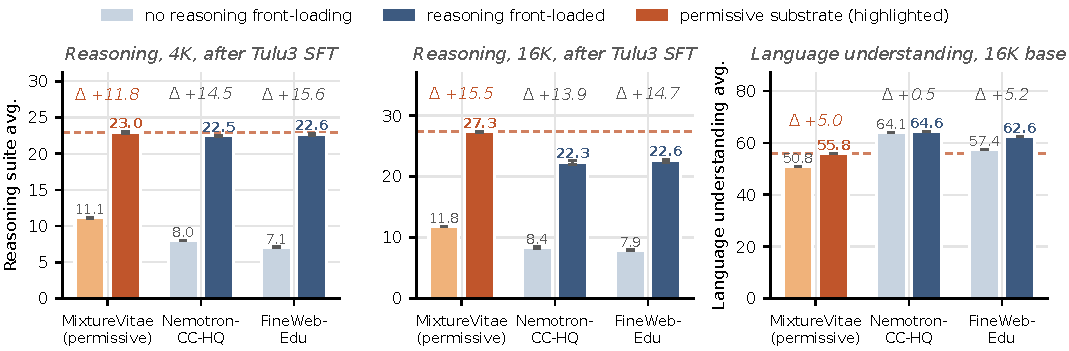
\includegraphics[width=\linewidth]{figures/factorial_main.pdf}
\caption{\textbf{Front-loading drives the reasoning gain and licensing does not.} Paired bars give the suite average without and with the instruction-and-reasoning subset in pre-training, for each web substrate, after Tulu3 SFT. The permissive substrate is highlighted, and the dashed line marks its front-loaded level so that the substrate contrast at matched front-loading can be read directly. Error bars are the sample standard deviation over three decoding seeds. Language understanding is single seed and measured on the base checkpoints.}
\label{fig:factorial}
\end{figure}

\paragraph{Front-loading is the operative variable.}
\Cref{tab:factorial} and \Cref{fig:factorial} give the design. Adding the instruction-and-reasoning subset to the pre-training mixture raises the reasoning suite average in all eighteen cells, by $10.3$ to $19.2$ points, with every bootstrap interval excluding zero at $q < 0.001$. At 16K after Tulu3 SFT the effect is $+15.5$ points for the permissive substrate ($11.8 \to 27.3$), $+13.9$ for Nemotron-CC-HQ ($8.4 \to 22.3$), and $+14.7$ for FineWeb-Edu ($7.9 \to 22.6$). It is largest at the base stage, near $19$ points for every substrate at 16K, and Phase 1 recovers only part of the deficit its absence creates. Tulu3 contains instruction, mathematics, and code data of its own, and applying it to a base without front-loaded reasoning does not substitute for having pre-trained on it.

\paragraph{Licensing is nearly free on reasoning.}
Once both pools are front-loaded the substrate contrast largely disappears. At 4K after Tulu3 SFT the permissive substrate leads Nemotron-CC-HQ by $+0.5$ points ($[-1.2, +2.3]$, $q = 0.65$) and FineWeb-Edu by $+0.4$ points ($[-1.3, +1.9]$, $q = 0.66$), both indistinguishable from zero, and at 16K it leads by $+5.0$ ($[+3.2, +7.0]$) and $+4.7$ points ($[+3.0, +6.6]$), both with $q \le 0.001$. The only stage at which a non-permissive substrate is ahead is the 4K base, before any post-training, where it leads by $5.4$ to $7.5$ points. Post-training removes that advantage rather than preserving it.

\paragraph{The mechanism does not depend on licensing.}
The interaction between the two factors, the front-loading effect on the permissive substrate minus its mean effect on the two non-permissive substrates, is $+0.0$ points at the 16K base ($[-2.0, +2.0]$, $q = 0.97$), $+1.2$ after SFT ($[-0.8, +3.2]$, $q = 0.28$), and $+1.9$ after DPO ($[-0.1, +4.0]$, $q = 0.10$), none distinguishable from zero. The effect is the same size wherever it is applied, which is what supports reading front-loading as the mechanism and licensing as a separate constraint.

\paragraph{The gains are broad.}
Averaged over the three substrates at 16K after SFT, front-loading is worth $+23.0$ points on code, $+15.6$ on mathematics, $+10.4$ on instruction following, and $+2.5$ on science and knowledge-intensive question answering (\Cref{fig:domains}), and instruction following improves in all twelve post-training cells, by $7.7$ to $17.5$ points. Because an unweighted average over five mathematics and three code benchmarks implicitly weights those domains at 45\% and 27\%, we recompute both headline quantities under an equal-domain average and with each domain removed in turn, and neither changes materially (\Cref{tab:domain_robustness}).

\paragraph{Language understanding is where the constraint is not free.}
Front-loading also helps general language understanding, by $+5.0$ points for the permissive substrate ($50.8 \to 55.8$ at 16K) and $+5.2$ for FineWeb-Edu ($57.4 \to 62.6$), though only $+0.5$ for Nemotron-CC-HQ, which already contains synthetically rephrased question-and-answer text and starts much higher. The instructive detail is what the non-front-loaded models cannot do. Without the subset, FineWeb-Edu and the permissive substrate score $26.1$ and $25.8$ on 5-shot MMLU and $21.1$ and $22.4$ on 10-shot CommonsenseQA, which is chance on both, and front-loading lifts them to $47.5$ and $38.7$ on MMLU and $55.7$ and $48.7$ on CommonsenseQA. Whatever else instruction and reasoning data supplies, it supplies the ability to answer a benchmark in the format the benchmark asks for.

It does not, however, close the substrate gap. At matched front-loading the permissive substrate reaches $55.8$ against $64.6$ for Nemotron-CC-HQ and $62.6$ for FineWeb-Edu, a residual $6.8$ to $8.8$ points that front-loading does not recover in our design. Permissiveness is close to free on the capabilities post-training targets and is not free on broad language coverage.

\section{Post-training across the model zoo}
\label{sec:zoo}

\begin{figure}[t]
\centering
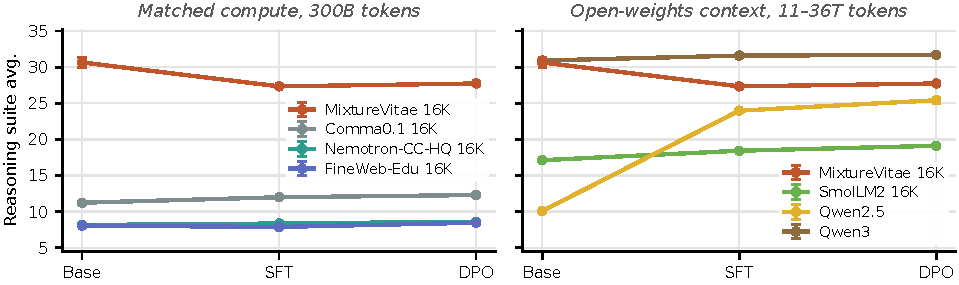
\includegraphics[width=\linewidth]{figures/phase1_zoo.pdf}
\caption{\textbf{Phase 1 trajectories, Protocol~A.} Left, matched-compute bases trained on 300B tokens under the \texttt{open-sci-ref} protocol. Right, the same permissive model against open-weights references trained on 36 to 120 times more tokens, shown as uncontrolled upper references. Error bars are the sample standard deviation over three decoding seeds. Per-benchmark values are in \Cref{tab:phase1_zoo}.}
\label{fig:zoo}
\end{figure}

% Generated by generate_workshop_artifacts.py. Do not edit by hand.
\begin{table}[t]
\centering
\caption{\textbf{Phase~1 across the model zoo.} One context variant per model family, namely the 16K variant where one exists and the released context otherwise. The matched-compute models are trained on 300B tokens under the \texttt{open-sci-ref} protocol, while SmolLM2, Qwen2.5, and Qwen3 use 11T, 18T, and 36T tokens respectively and are uncontrolled upper references. Both context variants of every model are in Table~\ref{tab:phase1_zoo_full}. Protocol~A (Appendix Table~\ref{tab:eval-settings-A}). Values are mean$_{\pm\text{SD}}$ over decoding seeds 42, 1234, and 2025.}
\label{tab:phase1_zoo}
\scriptsize
\setlength{\tabcolsep}{3pt}
\resizebox{\linewidth}{!}{%
\begin{tabular}{lrrrrrrrrrrrr}
\toprule
\textbf{Model} & \textbf{A24} & \textbf{A25} & \textbf{AMC} & \textbf{M500} & \textbf{GSM8K} & \textbf{HE} & \textbf{LCB} & \textbf{MBPP} & \textbf{GPQA} & \textbf{JEE} & \textbf{IFE} & \textbf{Avg} \\
\midrule
\addlinespace[0.15em]
\multicolumn{13}{l}{\textit{Matched compute, 300B tokens, controlled comparison}} \\
\addlinespace[0.2em]
MixtureVitae-16K & 1.1$_{\pm1.92}$ & 3.3$_{\pm0.00}$ & 23.3$_{\pm8.04}$ & 47.0$_{\pm0.53}$ & 60.0$_{\pm0.00}$ & 54.1$_{\pm0.35}$ & 22.3$_{\pm0.34}$ & 40.1$_{\pm0.23}$ & 23.4$_{\pm0.29}$ & 8.0$_{\pm0.24}$ & 54.6$_{\pm0.23}$ & 30.7$_{\pm0.72}$ \\
\quad $\to$ SFT & 3.3$_{\pm0.00}$ & 3.3$_{\pm0.00}$ & 15.0$_{\pm0.00}$ & 35.0$_{\pm0.53}$ & 51.6$_{\pm0.00}$ & 54.1$_{\pm0.35}$ & 14.4$_{\pm0.11}$ & 40.4$_{\pm0.35}$ & 23.4$_{\pm0.29}$ & 5.1$_{\pm0.27}$ & 55.1$_{\pm0.26}$ & 27.3$_{\pm0.11}$ \\
\quad $\to$ SFT $\to$ DPO & 3.3$_{\pm0.00}$ & 1.1$_{\pm1.92}$ & 17.5$_{\pm0.00}$ & 37.0$_{\pm0.80}$ & 52.6$_{\pm0.00}$ & 52.6$_{\pm0.70}$ & 14.6$_{\pm0.30}$ & 40.3$_{\pm0.12}$ & 23.4$_{\pm0.29}$ & 6.2$_{\pm0.20}$ & 56.5$_{\pm0.74}$ & 27.8$_{\pm0.04}$ \\
\midrule
\addlinespace[0.2em]
Nemotron-CC-HQ-16K & 0.0$_{\pm0.00}$ & 0.0$_{\pm0.00}$ & 0.0$_{\pm0.00}$ & 2.8$_{\pm0.35}$ & 8.2$_{\pm0.00}$ & 1.8$_{\pm0.00}$ & 0.1$_{\pm0.11}$ & 5.7$_{\pm0.31}$ & 22.7$_{\pm0.51}$ & 5.6$_{\pm1.04}$ & 42.7$_{\pm0.38}$ & 8.1$_{\pm0.08}$ \\
\quad $\to$ SFT & 0.0$_{\pm0.00}$ & 0.0$_{\pm0.00}$ & 0.0$_{\pm0.00}$ & 2.9$_{\pm0.31}$ & 8.6$_{\pm0.00}$ & 5.3$_{\pm0.35}$ & 0.0$_{\pm0.00}$ & 5.9$_{\pm0.12}$ & 22.2$_{\pm0.87}$ & 1.2$_{\pm0.08}$ & 45.8$_{\pm0.00}$ & 8.4$_{\pm0.12}$ \\
\quad $\to$ SFT $\to$ DPO & 0.0$_{\pm0.00}$ & 0.0$_{\pm0.00}$ & 2.5$_{\pm0.00}$ & 2.5$_{\pm0.12}$ & 7.7$_{\pm0.00}$ & 5.3$_{\pm0.35}$ & 0.0$_{\pm0.00}$ & 5.3$_{\pm0.12}$ & 23.4$_{\pm1.17}$ & 1.7$_{\pm0.37}$ & 46.3$_{\pm0.61}$ & 8.6$_{\pm0.06}$ \\
\midrule
\addlinespace[0.2em]
FineWeb-Edu-16K & 0.0$_{\pm0.00}$ & 0.0$_{\pm0.00}$ & 2.5$_{\pm0.00}$ & 2.9$_{\pm0.12}$ & 8.6$_{\pm0.00}$ & 2.4$_{\pm0.00}$ & 0.1$_{\pm0.11}$ & 2.0$_{\pm0.00}$ & 24.9$_{\pm0.29}$ & 6.5$_{\pm0.58}$ & 38.8$_{\pm0.53}$ & 8.1$_{\pm0.09}$ \\
\quad $\to$ SFT & 0.0$_{\pm0.00}$ & 0.0$_{\pm0.00}$ & 0.0$_{\pm0.00}$ & 3.1$_{\pm0.12}$ & 8.7$_{\pm0.00}$ & 4.9$_{\pm0.00}$ & 0.2$_{\pm0.00}$ & 2.5$_{\pm0.23}$ & 23.6$_{\pm0.58}$ & 2.4$_{\pm0.40}$ & 41.3$_{\pm0.46}$ & 7.9$_{\pm0.07}$ \\
\quad $\to$ SFT $\to$ DPO & 0.0$_{\pm0.00}$ & 3.3$_{\pm0.00}$ & 0.0$_{\pm0.00}$ & 3.3$_{\pm0.12}$ & 9.2$_{\pm0.00}$ & 4.9$_{\pm0.00}$ & 0.0$_{\pm0.00}$ & 2.5$_{\pm0.12}$ & 23.9$_{\pm0.29}$ & 2.7$_{\pm0.54}$ & 43.3$_{\pm0.57}$ & 8.5$_{\pm0.09}$ \\
\midrule
\addlinespace[0.2em]
DCLM & 0.0$_{\pm0.00}$ & 0.0$_{\pm0.00}$ & 0.0$_{\pm0.00}$ & 0.2$_{\pm0.00}$ & 3.0$_{\pm0.00}$ & 0.0$_{\pm0.00}$ & 0.0$_{\pm0.00}$ & 0.0$_{\pm0.00}$ & 19.5$_{\pm0.77}$ & 0.0$_{\pm0.00}$ & 39.2$_{\pm0.08}$ & 5.6$_{\pm0.08}$ \\
\quad $\to$ SFT & 0.0$_{\pm0.00}$ & 0.0$_{\pm0.00}$ & 0.0$_{\pm0.00}$ & 0.8$_{\pm0.00}$ & 5.2$_{\pm0.00}$ & 6.7$_{\pm0.00}$ & 0.2$_{\pm0.00}$ & 5.4$_{\pm0.35}$ & 21.7$_{\pm0.00}$ & 1.1$_{\pm0.49}$ & 40.6$_{\pm0.13}$ & 7.4$_{\pm0.02}$ \\
\quad $\to$ SFT $\to$ DPO & 0.0$_{\pm0.00}$ & 0.0$_{\pm0.00}$ & 1.7$_{\pm1.44}$ & 1.1$_{\pm0.23}$ & 4.6$_{\pm0.00}$ & 6.7$_{\pm0.00}$ & 0.3$_{\pm0.11}$ & 5.6$_{\pm0.00}$ & 20.7$_{\pm0.00}$ & 0.5$_{\pm0.03}$ & 43.0$_{\pm0.08}$ & 7.7$_{\pm0.15}$ \\
\midrule
\addlinespace[0.2em]
Comma0.1-16K & 0.0$_{\pm0.00}$ & 0.0$_{\pm0.00}$ & 1.7$_{\pm1.44}$ & 2.8$_{\pm0.35}$ & 12.2$_{\pm0.00}$ & 13.4$_{\pm0.00}$ & 0.1$_{\pm0.11}$ & 16.0$_{\pm0.20}$ & 25.8$_{\pm1.01}$ & 7.8$_{\pm0.19}$ & 43.8$_{\pm0.81}$ & 11.2$_{\pm0.22}$ \\
\quad $\to$ SFT & 0.0$_{\pm0.00}$ & 0.0$_{\pm0.00}$ & 2.5$_{\pm0.00}$ & 2.5$_{\pm0.12}$ & 6.9$_{\pm0.00}$ & 16.5$_{\pm0.00}$ & 1.4$_{\pm0.20}$ & 25.2$_{\pm0.35}$ & 23.2$_{\pm0.00}$ & 4.8$_{\pm0.66}$ & 49.0$_{\pm0.27}$ & 12.0$_{\pm0.01}$ \\
\quad $\to$ SFT $\to$ DPO & 0.0$_{\pm0.00}$ & 0.0$_{\pm0.00}$ & 2.5$_{\pm0.00}$ & 2.1$_{\pm0.12}$ & 6.7$_{\pm0.00}$ & 17.1$_{\pm0.00}$ & 1.8$_{\pm0.23}$ & 25.9$_{\pm0.31}$ & 23.4$_{\pm0.29}$ & 5.1$_{\pm0.12}$ & 50.6$_{\pm0.23}$ & 12.3$_{\pm0.03}$ \\
\midrule
\addlinespace[0.15em]
\multicolumn{13}{l}{\textit{External open-weights references, 11--36T tokens, uncontrolled}} \\
\addlinespace[0.2em]
SmolLM2-16K & 0.0$_{\pm0.00}$ & 0.0$_{\pm0.00}$ & 0.8$_{\pm1.44}$ & 11.8$_{\pm0.92}$ & 31.9$_{\pm0.00}$ & 24.0$_{\pm0.35}$ & 1.2$_{\pm0.23}$ & 36.5$_{\pm0.12}$ & 24.6$_{\pm0.29}$ & 7.6$_{\pm0.39}$ & 49.9$_{\pm0.27}$ & 17.1$_{\pm0.07}$ \\
\quad $\to$ SFT & 0.0$_{\pm0.00}$ & 0.0$_{\pm0.00}$ & 1.7$_{\pm1.44}$ & 9.6$_{\pm0.20}$ & 32.8$_{\pm0.00}$ & 32.9$_{\pm0.61}$ & 4.4$_{\pm0.11}$ & 37.5$_{\pm0.23}$ & 24.9$_{\pm1.91}$ & 4.7$_{\pm0.72}$ & 54.4$_{\pm0.40}$ & 18.4$_{\pm0.05}$ \\
\quad $\to$ SFT $\to$ DPO & 0.0$_{\pm0.00}$ & 0.0$_{\pm0.00}$ & 3.3$_{\pm1.44}$ & 9.6$_{\pm0.53}$ & 33.8$_{\pm0.00}$ & 32.3$_{\pm1.06}$ & 5.3$_{\pm0.20}$ & 36.9$_{\pm0.50}$ & 26.3$_{\pm0.00}$ & 5.4$_{\pm0.69}$ & 57.4$_{\pm0.20}$ & 19.1$_{\pm0.17}$ \\
\midrule
\addlinespace[0.2em]
Qwen2.5 & 0.0$_{\pm0.00}$ & 0.0$_{\pm0.00}$ & 0.0$_{\pm0.00}$ & 0.2$_{\pm0.35}$ & 61.9$_{\pm0.00}$ & 5.7$_{\pm0.70}$ & 0.2$_{\pm0.00}$ & 0.1$_{\pm0.12}$ & 11.1$_{\pm1.82}$ & 0.3$_{\pm0.10}$ & 31.3$_{\pm0.34}$ & 10.1$_{\pm0.15}$ \\
\quad $\to$ SFT & 3.3$_{\pm0.00}$ & 0.0$_{\pm0.00}$ & 8.3$_{\pm1.44}$ & 18.8$_{\pm0.69}$ & 39.0$_{\pm0.00}$ & 51.0$_{\pm0.35}$ & 8.0$_{\pm0.23}$ & 44.3$_{\pm0.23}$ & 29.0$_{\pm0.77}$ & 6.1$_{\pm0.54}$ & 56.0$_{\pm0.27}$ & 24.0$_{\pm0.07}$ \\
\quad $\to$ SFT $\to$ DPO & 2.2$_{\pm1.92}$ & 0.0$_{\pm0.00}$ & 10.0$_{\pm2.50}$ & 21.2$_{\pm1.00}$ & 40.4$_{\pm0.00}$ & 55.7$_{\pm0.70}$ & 8.5$_{\pm0.23}$ & 44.5$_{\pm0.23}$ & 27.9$_{\pm0.58}$ & 8.0$_{\pm0.64}$ & 61.2$_{\pm0.30}$ & 25.4$_{\pm0.40}$ \\
\midrule
\addlinespace[0.2em]
Qwen3 & 3.3$_{\pm0.00}$ & 2.2$_{\pm1.92}$ & 20.8$_{\pm3.82}$ & 48.0$_{\pm0.35}$ & 71.6$_{\pm0.00}$ & 64.2$_{\pm0.93}$ & 1.6$_{\pm0.11}$ & 46.5$_{\pm0.81}$ & 25.1$_{\pm0.77}$ & 18.0$_{\pm0.76}$ & 38.8$_{\pm0.34}$ & 30.9$_{\pm0.31}$ \\
\quad $\to$ SFT & 0.0$_{\pm0.00}$ & 0.0$_{\pm0.00}$ & 16.7$_{\pm2.89}$ & 28.2$_{\pm0.35}$ & 69.4$_{\pm0.00}$ & 67.1$_{\pm0.61}$ & 3.5$_{\pm0.85}$ & 54.3$_{\pm0.58}$ & 33.0$_{\pm1.05}$ & 11.9$_{\pm0.54}$ & 63.7$_{\pm0.13}$ & 31.6$_{\pm0.30}$ \\
\quad $\to$ SFT $\to$ DPO & 0.0$_{\pm0.00}$ & 0.0$_{\pm0.00}$ & 8.3$_{\pm1.44}$ & 31.2$_{\pm1.06}$ & 69.8$_{\pm0.00}$ & 67.7$_{\pm0.61}$ & 4.9$_{\pm0.00}$ & 54.7$_{\pm0.23}$ & 31.3$_{\pm0.87}$ & 13.3$_{\pm1.25}$ & 67.6$_{\pm1.33}$ & 31.7$_{\pm0.21}$ \\
\bottomrule
\end{tabular}}
\end{table}


\paragraph{The factorial result survives the wider comparison.}
\Cref{fig:zoo} and \Cref{tab:phase1_zoo} place the front-loaded permissive model against the bases the community actually trains on. After Phase 1 at 16K it reaches $27.8$, against $12.3$ for Comma0.1, $8.6$ for Nemotron-CC-HQ, and $8.5$ for FineWeb-Edu at the same 300B budget, and $7.7$ for DCLM at 4K. Comma0.1 is the informative comparison, since it is permissively licensed but not reasoning enriched, and it sits with the non-permissive references rather than with the front-loaded model. Licensing does not predict the ranking and composition does. Against the external references it exceeds SmolLM2 at 16K ($19.1$) and Qwen2.5 ($25.4$) and trails Qwen3 ($31.7$), which uses 120 times the tokens and whose pre-training already includes reasoning traces.

\paragraph{Short-context alignment erodes long-context reasoning.}
The permissive 16K model is strongest before Phase 1, at $30.7$, and Tulu3 SFT lowers it to $27.3$, with DPO recovering to $27.8$ but not to the base level. This is a degradation of an unusually strong post-extension base rather than a weak post-trained model, since the result still leads every matched-compute reference by more than 15 points. The natural reading is that the short-context-dominated Tulu3 mixture partially overwrites reasoning behavior that long-context extension and reasoning-rich pre-training installed, and \Cref{sec:receptivity} tests that reading directly. The same pattern is visible for Qwen3, whose base leads its own post-trained checkpoints on MATH500, so it is not specific to one mixture.

\paragraph{Which subset carries the signal.}
A mixture-composition ablation at a 100B-token budget isolates the two largest subsets of the permissive mixture (\Cref{tab:evalchemy_table1,tab:lang_eval_table1}). Removing the instruction-and-reasoning subset collapses the post-trained model to a suite average of 6 to 9 across contexts and stages, well below the full mixture, and Tulu3 does not repair it, which is the 100B counterpart of the front-loading effect in \Cref{sec:factorial}. Removing the curated web subset instead leaves both axes close to the full mixture and on several benchmarks above it, and costs about a point of mean accuracy on language understanding. At this budget the reasoning and instruction core carries most of the post-training signal and the web portion contributes comparatively little, though we state this only for the scale and budget tested.

\section{Receptivity to reasoning post-training}
\label{sec:receptivity}

Everything in this section is measured under Protocol~B at a single seed, so every number below is a change from a starting checkpoint re-evaluated under that protocol rather than a score comparable with \Cref{sec:factorial,sec:zoo}.

\begin{figure}[t]
\centering
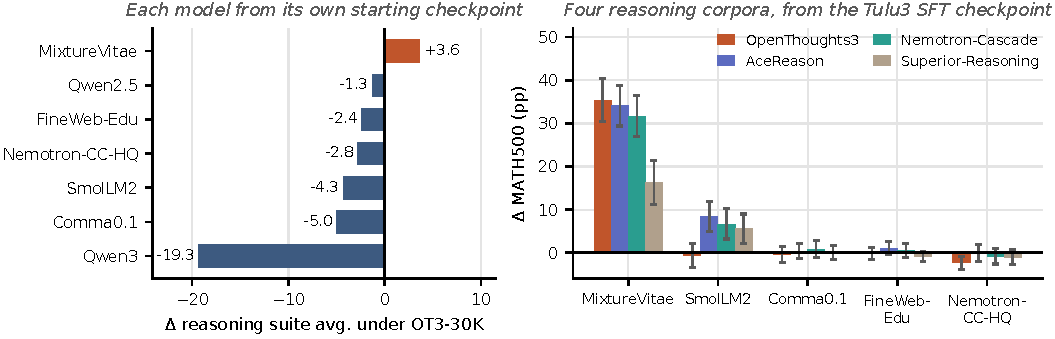
\includegraphics[width=\linewidth]{figures/phase2_receptivity.pdf}
\caption{\textbf{Only the front-loaded permissive base converts a small reasoning budget into gains.} Left, change in suite average under identical OpenThoughts3-30K post-training, measured for each model from its own Tulu3 SFT checkpoint, except MixtureVitae, which is measured from its post-YaRN base. Right, change in MATH500 when the Tulu3 SFT checkpoint of five bases receives 30K samples from one of four reasoning corpora, with 95\% paired bootstrap intervals over the same 500 problems. Protocol~B, single seed.}
\label{fig:receptivity}
\end{figure}

\paragraph{A small reasoning budget helps one base and harms the rest.}
Under an identical 30K-sample OpenThoughts3 update, the front-loaded permissive base is the only model in our study whose suite average rises, by $+3.6$ points from its post-YaRN base (\Cref{fig:receptivity}, \Cref{tab:phase2_endpoints}). Every other base declines from its own starting checkpoint, by $-1.3$ for Qwen2.5, $-2.4$ for FineWeb-Edu, $-2.8$ for Nemotron-CC-HQ, $-4.3$ for SmolLM2, $-5.0$ for Comma0.1, and $-19.3$ for Qwen3. We read Qwen3's decline as reduced susceptibility at a budget this small, since a recipe or budget mismatch would produce the same signature. The same update also recovers the long-context mathematics performance that Phase 1 erodes in \Cref{sec:zoo}, and does so from the base checkpoint without any Tulu3 stage, which supports reading that erosion as short-context interference.

\paragraph{Removing the reasoning traces from pre-training removes the receptivity.}
\Cref{tab:ot3_pretrain_ablation} isolates this at the full 300B budget. Two models differ only in whether the OpenThoughts3 subset is present in pre-training, and both receive identical reasoning post-training. With it the suite average reaches $33.6$, and without it the same post-training reaches $23.9$, below the level the intact base already had before any reasoning update. The gap is $31.8$ points on MATH500, $30.0$ on AMC23, and $19.5$ on HumanEval, and AIME24 and AIME25 fall from $11.7$ and $10.0$ to exactly zero. Post-training amplified a capability that pre-training had laid down, and where it had not there was nothing to amplify.

% Generated by generate_workshop_artifacts.py. Do not edit by hand.
\begin{table}[t]
\centering
\caption{\textbf{Removing OpenThoughts3 from pre-training removes the receptivity to reasoning post-training.} Two 1.7B models pre-trained on 300B tokens that differ only in whether the OpenThoughts3 subset is present, then given the identical OT3-30K reasoning post-training. Architecture, schedule, token budget, long-context extension, post-training recipe, and evaluation are held fixed. The intact base is shown as a reference level, and the two post-trained endpoints are the comparison. Bold marks the condition of interest, the model whose pre-training retained OpenThoughts3. Protocol~B, the reasoning post-training protocol (Appendix Table~\ref{tab:eval-settings-B}). Single seed, so no error bars are available.}
\label{tab:ot3_pretrain_ablation}
\small
\setlength{\tabcolsep}{3.5pt}
\resizebox{\linewidth}{!}{%
\begin{tabular}{lrrrrrrrrrrrr}
\toprule
\textbf{300B model} & \textbf{A24} & \textbf{A25} & \textbf{AMC} & \textbf{M500} & \textbf{GSM8K} & \textbf{HE} & \textbf{LCB} & \textbf{MBPP} & \textbf{GPQA} & \textbf{JEE} & \textbf{IFE} & \textbf{Avg} \\
\midrule
Base with OT3, before reasoning post-training & 3.3 & 8.3 & 25.6 & 34.6 & 54.1 & 42.1 & 8.4 & 29.2 & 27.3 & 10.2 & 45.2 & 26.2 \\
\midrule
OT3 in pre-training, $\to$ OT30K & \textbf{11.7} & \textbf{10.0} & \textbf{47.5} & \textbf{69.8} & \textbf{56.4} & \textbf{57.9} & \textbf{12.7} & \textbf{26.6} & \textbf{28.3} & \textbf{20.6} & \textbf{27.6} & \textbf{33.6} \\
OT3 removed from pre-training, $\to$ OT30K & 0.0 & 0.0 & 17.5 & 38.0 & 53.3 & 38.4 & 6.2 & 33.8 & 28.8 & 11.0 & 36.4 & 23.9 \\
\bottomrule
\end{tabular}}
\end{table}


\paragraph{The effect is not an artifact of training twice on the same corpus.}
Because OpenThoughts3 traces are present in the permissive pre-training mixture, its gain under OpenThoughts3 post-training could reflect re-exposure rather than receptivity. \Cref{tab:heldout_reasoning} holds the intervention fixed and changes only the identity of the reasoning corpus. From the Tulu3 SFT checkpoint the permissive base gains $+35.4$ points of MATH500 under OpenThoughts3 and $+34.2$, $+31.6$, and $+16.4$ under AceReason, Nemotron-Cascade, and Superior-Reasoning, three corpora that are not named sources in any pre-training mixture here, with every interval excluding zero. No matched-compute reference responds positively to any of the four, and SmolLM2, which is neither compute matched nor trained under our recipe, responds to three of the four roughly three to five times more weakly, and not at all to OpenThoughts3. Receptivity is therefore a property of the base rather than of the post-training corpus, although the corpus shapes the profile of the gain, with Superior-Reasoning improving mathematics while regressing code and instruction following enough to lower the average (\Cref{tab:heldout_mv_grid}).

% Generated by generate_workshop_artifacts.py. Do not edit by hand.
\begin{table}[t]
\centering
\caption{\textbf{The reasoning gain is not tied to OpenThoughts3.} Change in MATH500 accuracy when each base's Tulu3 SFT checkpoint receives 30K samples from one of four reasoning corpora, three of which are absent from every pre-training mixture considered here. Brackets are 95\% paired bootstrap intervals over the same 500 problems. \textbf{Bold} marks a significant increase and \emph{italic} a significant decrease after Benjamini--Hochberg correction. Protocol~B, the reasoning post-training protocol (Appendix Table~\ref{tab:eval-settings-B}). Single seed, so no error bars are available.}
\label{tab:heldout_reasoning}
\small
\setlength{\tabcolsep}{4pt}
\resizebox{\linewidth}{!}{%
\begin{tabular}{lrrrr}
\toprule
\textbf{Base} & \textbf{OpenThoughts3} & \textbf{AceReason} & \textbf{Nemotron-Cascade} & \textbf{Superior-Reasoning} \\
\midrule
MixtureVitae & $\bm{+35.4}$ {\scriptsize$[+30.4, +40.4]$} & $\bm{+34.2}$ {\scriptsize$[+29.4, +38.8]$} & $\bm{+31.6}$ {\scriptsize$[+27.0, +36.4]$} & $\bm{+16.4}$ {\scriptsize$[+11.2, +21.4]$} \\
\midrule
Comma0.1 & $-0.4$ {\scriptsize$[-2.2, +1.4]$} & $+0.4$ {\scriptsize$[-1.4, +2.2]$} & $+0.8$ {\scriptsize$[-1.2, +2.8]$} & $+0.0$ {\scriptsize$[-1.6, +1.6]$} \\
FineWeb-Edu & $-0.2$ {\scriptsize$[-1.6, +1.2]$} & $+1.0$ {\scriptsize$[-0.4, +2.6]$} & $+0.6$ {\scriptsize$[-1.0, +2.2]$} & $-0.8$ {\scriptsize$[-2.0, +0.4]$} \\
Nemotron-CC-HQ & \emph{$-2.2$} {\scriptsize$[-3.8, -0.8]$} & $+0.0$ {\scriptsize$[-2.0, +2.0]$} & $-0.8$ {\scriptsize$[-2.6, +1.0]$} & $-1.0$ {\scriptsize$[-2.8, +0.8]$} \\
SmolLM2 & $-0.6$ {\scriptsize$[-3.4, +2.2]$} & $\bm{+8.4}$ {\scriptsize$[+5.0, +11.8]$} & $\bm{+6.6}$ {\scriptsize$[+3.2, +10.2]$} & $\bm{+5.6}$ {\scriptsize$[+2.2, +9.0]$} \\
\bottomrule
\end{tabular}}
\end{table}


\paragraph{What reasoning post-training costs.}
Instruction following is a control here rather than a target, and it declines under every reasoning update, since the post-training data contains none. Running DPO before the reasoning stage largely preserves it, at $43.0$ against $45.0$ before. General language understanding does not degrade, reading $56.0$ after the reasoning update from either starting point against $55.0$ through Phase 1 (\Cref{tab:lang_eval_table2,tab:lang_eval_ot3_phase2}). More broadly the average over the non-mathematics benchmarks falls in most of these runs, so the gain from a small reasoning budget is real but concentrated, and is bought at a measurable cost in instruction following rather than in general language.

\section{Related work}
\label{sec:related_work}

\textbf{Permissive pre-training corpora.} CommonCorpus~\citep{langlais2025commoncorpus} assembles roughly 2T tokens of uncopyrighted and permissively licensed text, and CommonPile~\citep{kandpal2025commonpilev018tb_arxiv} builds pre-training corpora exclusively from permissively licensed sources. MixtureVitae~\citep{nguyen2025mixturevitae_arxiv} showed that much of the gap to mixed-license corpora closes at the base-model stage when a large instruction and reasoning fraction is included, and SYNTH~\citep{synthpleias2025} pursues a related synthetic route. None of these varies licensing and composition independently, which is what this paper adds.

\textbf{Quality-filtered web corpora.} FineWeb-Edu~\citep{penedo2024fineweb} filters for educational value, and Nemotron-CC~\citep{su2025nemotroncctransformingcommoncrawl} combines classifier ensembles with synthetic rephrasing. The \texttt{open-sci-ref} protocol~\citep{nezhurina2025opensciref} established the reference recipe we use and identified Nemotron-CC-HQ~\citep{blakeman2025nemotron} as the strongest such corpus, ahead of DCLM~\citep{li2024datacomplm} and FineWeb-Edu.

\textbf{Instruction and reasoning data in pre-training.} Phi-1~\citep{gunasekar2023phi1} showed that textbook-quality and synthetic exercise data can carry a small model to strong code performance. Front-Loaded Reasoning~\citep{akter2025front} makes the pre-training-side case that reasoning data introduced early establishes capabilities that later supervised fine-tuning cannot fully replicate, and PRISM~\citep{runwal2026prism} and \citet{zhang2026interplay} reach compatible conclusions from mid-training. Our design differs in three ways that matter for attribution. Pre-training here is single stage, so no stage boundary, schedule change, or curriculum shift co-varies with the mixture. Pre-training and all shared post-training data are decontaminated against every reported benchmark, which matters because front-loading mathematics and code is the regime where leakage is most likely. And licensing is varied rather than held implicitly fixed at non-permissive.

\textbf{Post-training recipes.} OpenThoughts~\citep{guha2025openthoughts} provides the reasoning traces and the recipe we use, and Tulu3~\citep{lambert2024tulu} the instruction alignment recipe including DPO~\citep{rafailov2023direct}. LIMA~\citep{zhou2023lima} and LIMO~\citep{yelimo} argue that small post-training sets can elicit instruction following and mathematical reasoning from a well-pre-trained base, an amplification account they motivate but do not test by varying pre-training. A separate line induces reasoning through reinforcement learning with verifiable rewards or test-time scaling~\citep{guo2025deepseek,yu2025dapo,muennighoff2025s1}. Those papers vary the post-training algorithm or data. We hold post-training fixed and vary the pre-training mixture.

\section{Conclusion and limitations}
\label{sec:limitations}

Asked what a base model must contain for post-training to succeed, this design answers with the pre-training mixture rather than the pre-training licence. Front-loading is worth 10 to 19 points of reasoning suite average in every cell of a 300B-token factorial, works equally well on permissive and non-permissive substrates, and helps broadly across mathematics, code, and instruction following. Under a permissive-data constraint the mechanism stays available essentially in full on the capabilities post-training targets and incomplete on general language coverage. For a community that wants to share data, recipes, and checkpoints without legal friction, that constraint is affordable, and composition rather than licensing is where the capability is decided.


\textbf{Scale and substrate.} All factorial results are at 1.7B parameters and 300B tokens, with a 0.4B cross-check in \Cref{app:smallscale}, and the licensing factor has a single permissive level, so ``permissive'' here means MixtureVitae specifically. The same factorial at 7B and above, with CommonPile and CommonCorpus added as further levels, would turn a two-level contrast into a properly sampled factor and test whether the near-zero licensing penalty survives scale. This is the most valuable follow-up and the one we can least afford.

\textbf{Post-training family.} We test Tulu3 SFT and DPO and a 30K-sample reasoning update, without Tulu3's reinforcement learning stage. Concluding that a weak mixture is genuinely unrecoverable would need exactly the regimes we omit, namely reinforcement learning with verifiable rewards and larger reasoning budgets, so we claim only that the deficit is not recovered under the recipes tested.

\textbf{Measurement and coverage.} Our intervals describe evaluation variability conditional on fixed checkpoints, so separating mixture effects from initialization variance needs replicate pre-training runs. The suite omits multilinguality, long-context retrieval, and tool use.

\textbf{The language gap is open.} Front-loading does not close the substrate gap on general language understanding, and whether targeted composition on a permissive substrate can is the most direct follow-up to the one negative result in this paper.

\bibliographystyle{plainnat}
\bibliography{add_reference,references}

%%%%%%%%%%%%%%%%%%%%%%%%%%%%%%%%%%%%%%%%%%%%%%%%%%%%%%%%%%%%

\newpage
\section*{NeurIPS Paper Checklist}

%%% BEGIN INSTRUCTIONS %%%
% The checklist is designed to encourage best practices for responsible machine learning research, addressing issues of reproducibility, transparency, research ethics, and societal impact. Do not remove the checklist: {\bf The papers not including the checklist will be desk rejected.} The checklist should follow the references and follow the (optional) supplemental material.  The checklist does NOT count towards the page
% limit. 

% Please read the checklist guidelines carefully for information on how to answer these questions. For each question in the checklist:
% \begin{itemize}
%     \item You should answer \answerYes{}, \answerNo{}, or \answerNA{}.
%     \item \answerNA{} means either that the question is Not Applicable for that particular paper or the relevant information is Not Available.
%     \item Please provide a short (1--2 sentence) justification right after your answer (even for \answerNA). 
%    % \item {\bf The papers not including the checklist will be desk rejected.}
% \end{itemize}

% {\bf The checklist answers are an integral part of your paper submission.} They are visible to the reviewers, area chairs, senior area chairs, and ethics reviewers. You will also be asked to include it (after eventual revisions) with the final version of your paper, and its final version will be published with the paper.

% The reviewers of your paper will be asked to use the checklist as one of the factors in their evaluation. While \answerYes{} is generally preferable to \answerNo{}, it is perfectly acceptable to answer \answerNo{} provided a proper justification is given (e.g., error bars are not reported because it would be too computationally expensive'' or ``we were unable to find the license for the dataset we used''). In general, answering \answerNo{} or \answerNA{} is not grounds for rejection. While the questions are phrased in a binary way, we acknowledge that the true answer is often more nuanced, so please just use your best judgment and write a justification to elaborate. All supporting evidence can appear either in the main paper or the supplemental material, provided in appendix. If you answer \answerYes{} to a question, in the justification please point to the section(s) where related material for the question can be found.

% IMPORTANT, please:
% \begin{itemize}
%     \item {\bf Delete this instruction block, but keep the section heading ``NeurIPS Paper Checklist"},
%     \item  {\bf Keep the checklist subsection headings, questions/answers and guidelines below.}
%     \item {\bf Do not modify the questions and only use the provided macros for your answers}.
% \end{itemize} 
 

%%% END INSTRUCTIONS %%%


\begin{enumerate}

\item {\bf Claims}
    \item[] Question: Do the main claims made in the abstract and introduction accurately reflect the paper's contributions and scope?
    \item[] Answer: \answerYes{} % Replace by \answerYes{}, \answerNo{}, or \answerNA{}.
    \item[] Justification: The abstract and Sec.~\ref{sec:intro} state four claims, mapping to Sec.~\ref{sec:factorial}, Sec.~\ref{sec:zoo}, and Sec.~\ref{sec:receptivity}, and they include the negative result that licensing is not free on general language understanding. Scope is bounded in Sec.~\ref{sec:limitations}.
    \item[] Guidelines:
    \begin{itemize}
        \item The answer \answerNA{} means that the abstract and introduction do not include the claims made in the paper.
        \item The abstract and/or introduction should clearly state the claims made, including the contributions made in the paper and important assumptions and limitations. A \answerNo{} or \answerNA{} answer to this question will not be perceived well by the reviewers. 
        \item The claims made should match theoretical and experimental results, and reflect how much the results can be expected to generalize to other settings. 
        \item It is fine to include aspirational goals as motivation as long as it is clear that these goals are not attained by the paper. 
    \end{itemize}

\item {\bf Limitations}
    \item[] Question: Does the paper discuss the limitations of the work performed by the authors?
    \item[] Answer: \answerYes{} % Replace by \answerYes{}, \answerNo{}, or \answerNA{}.
    \item[] Justification: See Sec.~\ref{sec:limitations}, which gives four limitations: model scale and the single permissive substrate, the post-training family tested, measurement and benchmark coverage, and the unresolved language gap. Each names the experiment that would resolve it.
    \item[] Guidelines:
    \begin{itemize}
        \item The answer \answerNA{} means that the paper has no limitation while the answer \answerNo{} means that the paper has limitations, but those are not discussed in the paper. 
        \item The authors are encouraged to create a separate ``Limitations'' section in their paper.
        \item The paper should point out any strong assumptions and how robust the results are to violations of these assumptions (e.g., independence assumptions, noiseless settings, model well-specification, asymptotic approximations only holding locally). The authors should reflect on how these assumptions might be violated in practice and what the implications would be.
        \item The authors should reflect on the scope of the claims made, e.g., if the approach was only tested on a few datasets or with a few runs. In general, empirical results often depend on implicit assumptions, which should be articulated.
        \item The authors should reflect on the factors that influence the performance of the approach. For example, a facial recognition algorithm may perform poorly when image resolution is low or images are taken in low lighting. Or a speech-to-text system might not be used reliably to provide closed captions for online lectures because it fails to handle technical jargon.
        \item The authors should discuss the computational efficiency of the proposed algorithms and how they scale with dataset size.
        \item If applicable, the authors should discuss possible limitations of their approach to address problems of privacy and fairness.
        \item While the authors might fear that complete honesty about limitations might be used by reviewers as grounds for rejection, a worse outcome might be that reviewers discover limitations that aren't acknowledged in the paper. The authors should use their best judgment and recognize that individual actions in favor of transparency play an important role in developing norms that preserve the integrity of the community. Reviewers will be specifically instructed to not penalize honesty concerning limitations.
    \end{itemize}

\item {\bf Theory assumptions and proofs}
    \item[] Question: For each theoretical result, does the paper provide the full set of assumptions and a complete (and correct) proof?
    \item[] Answer: \answerNA{} % Replace by \answerYes{}, \answerNo{}, or \answerNA{}.
    \item[] Justification: The paper contains no theoretical results.
    \item[] Guidelines:
    \begin{itemize}
        \item The answer \answerNA{} means that the paper does not include theoretical results. 
        \item All the theorems, formulas, and proofs in the paper should be numbered and cross-referenced.
        \item All assumptions should be clearly stated or referenced in the statement of any theorems.
        \item The proofs can either appear in the main paper or the supplemental material, but if they appear in the supplemental material, the authors are encouraged to provide a short proof sketch to provide intuition. 
        \item Inversely, any informal proof provided in the core of the paper should be complemented by formal proofs provided in appendix or supplemental material.
        \item Theorems and Lemmas that the proof relies upon should be properly referenced. 
    \end{itemize}

    \item {\bf Experimental result reproducibility}
    \item[] Question: Does the paper fully disclose all the information needed to reproduce the main experimental results of the paper to the extent that it affects the main claims and/or conclusions of the paper (regardless of whether the code and data are provided or not)?
    \item[] Answer: \answerYes{} % Replace by \answerYes{}, \answerNo{}, or \answerNA{}.
    \item[] Justification: Sec.~\ref{sec:methods} gives the factorial design, the pre-training configuration, the post-training recipes, and both evaluation protocols, and App.~\ref{appendix:exp_details} gives hyperparameters, protocol tables, and the decontamination procedure. Checkpoints and the pipeline that regenerates every table and figure from per-sample evaluation records will be released on acceptance.
    \item[] Guidelines:
    \begin{itemize}
        \item The answer \answerNA{} means that the paper does not include experiments.
        \item If the paper includes experiments, a \answerNo{} answer to this question will not be perceived well by the reviewers: Making the paper reproducible is important, regardless of whether the code and data are provided or not.
        \item If the contribution is a dataset and\slash or model, the authors should describe the steps taken to make their results reproducible or verifiable. 
        \item Depending on the contribution, reproducibility can be accomplished in various ways. For example, if the contribution is a novel architecture, describing the architecture fully might suffice, or if the contribution is a specific model and empirical evaluation, it may be necessary to either make it possible for others to replicate the model with the same dataset, or provide access to the model. In general. releasing code and data is often one good way to accomplish this, but reproducibility can also be provided via detailed instructions for how to replicate the results, access to a hosted model (e.g., in the case of a large language model), releasing of a model checkpoint, or other means that are appropriate to the research performed.
        \item While NeurIPS does not require releasing code, the conference does require all submissions to provide some reasonable avenue for reproducibility, which may depend on the nature of the contribution. For example
        \begin{enumerate}
            \item If the contribution is primarily a new algorithm, the paper should make it clear how to reproduce that algorithm.
            \item If the contribution is primarily a new model architecture, the paper should describe the architecture clearly and fully.
            \item If the contribution is a new model (e.g., a large language model), then there should either be a way to access this model for reproducing the results or a way to reproduce the model (e.g., with an open-source dataset or instructions for how to construct the dataset).
            \item We recognize that reproducibility may be tricky in some cases, in which case authors are welcome to describe the particular way they provide for reproducibility. In the case of closed-source models, it may be that access to the model is limited in some way (e.g., to registered users), but it should be possible for other researchers to have some path to reproducing or verifying the results.
        \end{enumerate}
    \end{itemize}


\item {\bf Open access to data and code}
    \item[] Question: Does the paper provide open access to the data and code, with sufficient instructions to faithfully reproduce the main experimental results, as described in supplemental material?
    \item[] Answer: \answerNo{} % Replace by \answerYes{}, \answerNo{}, or \answerNA{}.
    \item[] Justification: Releasing the checkpoints and the repository at submission time would break anonymity, so they are not available to reviewers. All base, long-context, SFT, DPO, and reasoning post-trained checkpoints, together with the artifact-generation pipeline, will be released on acceptance, as stated in Sec.~\ref{sec:intro}.
    \item[] Guidelines:
    \begin{itemize}
        \item The answer \answerNA{} means that paper does not include experiments requiring code.
        \item Please see the NeurIPS code and data submission guidelines (\url{https://neurips.cc/public/guides/CodeSubmissionPolicy}) for more details.
        \item While we encourage the release of code and data, we understand that this might not be possible, so \answerNo{} is an acceptable answer. Papers cannot be rejected simply for not including code, unless this is central to the contribution (e.g., for a new open-source benchmark).
        \item The instructions should contain the exact command and environment needed to run to reproduce the results. See the NeurIPS code and data submission guidelines (\url{https://neurips.cc/public/guides/CodeSubmissionPolicy}) for more details.
        \item The authors should provide instructions on data access and preparation, including how to access the raw data, preprocessed data, intermediate data, and generated data, etc.
        \item The authors should provide scripts to reproduce all experimental results for the new proposed method and baselines. If only a subset of experiments are reproducible, they should state which ones are omitted from the script and why.
        \item At submission time, to preserve anonymity, the authors should release anonymized versions (if applicable).
        \item Providing as much information as possible in supplemental material (appended to the paper) is recommended, but including URLs to data and code is permitted.
    \end{itemize}


\item {\bf Experimental setting/details}
    \item[] Question: Does the paper specify all the training and test details (e.g., data splits, hyperparameters, how they were chosen, type of optimizer) necessary to understand the results?
    \item[] Answer: \answerYes{} % Replace by \answerYes{}, \answerNo{}, or \answerNA{}.
    \item[] Justification: Sec.~\ref{sec:methods} gives the factorial design, the model zoo, and the post-training pipeline. App.~\ref{app:hyperparams} gives the \texttt{open-sci-ref} architecture and training schedules, App.~\ref{app:protocols} gives both evaluation protocols in full, and App.~\ref{app:decontam} gives the decontamination procedure.
    \item[] Guidelines:
    \begin{itemize}
        \item The answer \answerNA{} means that the paper does not include experiments.
        \item The experimental setting should be presented in the core of the paper to a level of detail that is necessary to appreciate the results and make sense of them.
        \item The full details can be provided either with the code, in appendix, or as supplemental material.
    \end{itemize}

\item {\bf Experiment statistical significance}
    \item[] Question: Does the paper report error bars suitably and correctly defined or other appropriate information about the statistical significance of the experiments?
    \item[] Answer: \answerYes{} % Replace by \answerYes{}, \answerNo{}, or \answerNA{}.
    \item[] Justification: All Protocol~A results report a mean and a sample standard deviation over three decoding seeds (42, 1234, 2025), and all contrasts on the suite average carry 95\% percentile intervals from a paired item-level bootstrap with 2{,}000 replicates, corrected with Benjamini--Hochberg within each contrast family. The factors of variability, the resampling scheme, and the small-sample caveat for the contest-mathematics benchmarks are stated in Sec.~\ref{sec:methods-bench} and App.~\ref{app:stats}. These intervals describe evaluation variability conditional on fixed checkpoints and do not estimate variability across independent pre-training runs, which is stated in Sec.~\ref{sec:limitations}. Protocol~B results are single seed and are reported without error bars, which every Protocol~B caption states.
    \item[] Guidelines:
    \begin{itemize}
        \item The answer \answerNA{} means that the paper does not include experiments.
        \item The authors should answer \answerYes{} if the results are accompanied by error bars, confidence intervals, or statistical significance tests, at least for the experiments that support the main claims of the paper.
        \item The factors of variability that the error bars are capturing should be clearly stated (for example, train/test split, initialization, random drawing of some parameter, or overall run with given experimental conditions).
        \item The method for calculating the error bars should be explained (closed form formula, call to a library function, bootstrap, etc.)
        \item The assumptions made should be given (e.g., Normally distributed errors).
        \item It should be clear whether the error bar is the standard deviation or the standard error of the mean.
        \item It is OK to report 1-sigma error bars, but one should state it. The authors should preferably report a 2-sigma error bar than state that they have a 96\% CI, if the hypothesis of Normality of errors is not verified.
        \item For asymmetric distributions, the authors should be careful not to show in tables or figures symmetric error bars that would yield results that are out of range (e.g., negative error rates).
        \item If error bars are reported in tables or plots, the authors should explain in the text how they were calculated and reference the corresponding figures or tables in the text.
    \end{itemize}

\item {\bf Experiments compute resources}
    \item[] Question: For each experiment, does the paper provide sufficient information on the computer resources (type of compute workers, memory, time of execution) needed to reproduce the experiments?
    \item[] Answer: \answerYes{} % Replace by \answerYes{}, \answerNo{}, or \answerNA{}.
    \item[] Justification: App.~\ref{appendix:exp_details} reports the hardware and single-run GPU-hours for reasoning post-training (Tab.~\ref{tab:ot30k_sft_gpu_hours}) and long-context extension (Tab.~\ref{tab:long_ctx_extension_gpu_hours}). Pre-training follows the \texttt{open-sci-ref} 1.7B configuration, whose architecture, per-token FLOPs, and token schedules are in Tab.~\ref{tab:opensciref_scales} and Tab.~\ref{tab:training_schedules}. We do not report per-run pre-training GPU-hours.
    \item[] Guidelines:
    \begin{itemize}
        \item The answer \answerNA{} means that the paper does not include experiments.
        \item The paper should indicate the type of compute workers CPU or GPU, internal cluster, or cloud provider, including relevant memory and storage.
        \item The paper should provide the amount of compute required for each of the individual experimental runs as well as estimate the total compute. 
        \item The paper should disclose whether the full research project required more compute than the experiments reported in the paper (e.g., preliminary or failed experiments that didn't make it into the paper). 
    \end{itemize}
    
\item {\bf Code of ethics}
    \item[] Question: Does the research conducted in the paper conform, in every respect, with the NeurIPS Code of Ethics \url{https://neurips.cc/public/EthicsGuidelines}?
    \item[] Answer: \answerYes{} % Replace by \answerYes{}, \answerNo{}, or \answerNA{}.
    \item[] Justification: The research conducted in this paper conforms with the NeurIPS Code of Ethics in every respect.
    \item[] Guidelines:
    \begin{itemize}
        \item The answer \answerNA{} means that the authors have not reviewed the NeurIPS Code of Ethics.
        \item If the authors answer \answerNo, they should explain the special circumstances that require a deviation from the Code of Ethics.
        \item The authors should make sure to preserve anonymity (e.g., if there is a special consideration due to laws or regulations in their jurisdiction).
    \end{itemize}


\item {\bf Broader impacts}
    \item[] Question: Does the paper discuss both potential positive societal impacts and negative societal impacts of the work performed?
    \item[] Answer: \answerYes{} % Replace by \answerYes{}, \answerNo{}, or \answerNA{}.
    \item[] Justification: See the broader impact statement at the start of the appendix.
    \item[] Guidelines:
    \begin{itemize}
        \item The answer \answerNA{} means that there is no societal impact of the work performed.
        \item If the authors answer \answerNA{} or \answerNo, they should explain why their work has no societal impact or why the paper does not address societal impact.
        \item Examples of negative societal impacts include potential malicious or unintended uses (e.g., disinformation, generating fake profiles, surveillance), fairness considerations (e.g., deployment of technologies that could make decisions that unfairly impact specific groups), privacy considerations, and security considerations.
        \item The conference expects that many papers will be foundational research and not tied to particular applications, let alone deployments. However, if there is a direct path to any negative applications, the authors should point it out. For example, it is legitimate to point out that an improvement in the quality of generative models could be used to generate Deepfakes for disinformation. On the other hand, it is not needed to point out that a generic algorithm for optimizing neural networks could enable people to train models that generate Deepfakes faster.
        \item The authors should consider possible harms that could arise when the technology is being used as intended and functioning correctly, harms that could arise when the technology is being used as intended but gives incorrect results, and harms following from (intentional or unintentional) misuse of the technology.
        \item If there are negative societal impacts, the authors could also discuss possible mitigation strategies (e.g., gated release of models, providing defenses in addition to attacks, mechanisms for monitoring misuse, mechanisms to monitor how a system learns from feedback over time, improving the efficiency and accessibility of ML).
    \end{itemize}
    
\item {\bf Safeguards}
    \item[] Question: Does the paper describe safeguards that have been put in place for responsible release of data or models that have a high risk for misuse (e.g., pre-trained language models, image generators, or scraped datasets)?
    \item[] Answer: \answerNA{} % Replace by \answerYes{}, \answerNo{}, or \answerNA{}.
    \item[] Justification: The released artifacts are 1.7B research checkpoints trained on public corpora, with no capability beyond comparable open releases, so no specific safeguard is required. The general dual-use considerations for open model releases are noted in the broader impact statement.
    \item[] Guidelines:
    \begin{itemize}
        \item The answer \answerNA{} means that the paper poses no such risks.
        \item Released models that have a high risk for misuse or dual-use should be released with necessary safeguards to allow for controlled use of the model, for example by requiring that users adhere to usage guidelines or restrictions to access the model or implementing safety filters. 
        \item Datasets that have been scraped from the Internet could pose safety risks. The authors should describe how they avoided releasing unsafe images.
        \item We recognize that providing effective safeguards is challenging, and many papers do not require this, but we encourage authors to take this into account and make a best faith effort.
    \end{itemize}

\item {\bf Licenses for existing assets}
    \item[] Question: Are the creators or original owners of assets (e.g., code, data, models), used in the paper, properly credited and are the license and terms of use explicitly mentioned and properly respected?
    \item[] Answer: \answerYes{} % Replace by \answerYes{}, \answerNo{}, or \answerNA{}.
    \item[] Justification: Licensing is the subject of the paper. Sec.~\ref{sec:methods-factorial} identifies which web substrates are permissive and which are not, and Sec.~\ref{sec:related_work} cites the originating release for every corpus. The post-training data (Tulu3, OpenThoughts3), the benchmark suites, and the evaluation harnesses are cited at first use and used under their published terms.
    \item[] Guidelines:
    \begin{itemize}
        \item The answer \answerNA{} means that the paper does not use existing assets.
        \item The authors should cite the original paper that produced the code package or dataset.
        \item The authors should state which version of the asset is used and, if possible, include a URL.
        \item The name of the license (e.g., CC-BY 4.0) should be included for each asset.
        \item For scraped data from a particular source (e.g., website), the copyright and terms of service of that source should be provided.
        \item If assets are released, the license, copyright information, and terms of use in the package should be provided. For popular datasets, \url{paperswithcode.com/datasets} has curated licenses for some datasets. Their licensing guide can help determine the license of a dataset.
        \item For existing datasets that are re-packaged, both the original license and the license of the derived asset (if it has changed) should be provided.
        \item If this information is not available online, the authors are encouraged to reach out to the asset's creators.
    \end{itemize}

\item {\bf New assets}
    \item[] Question: Are new assets introduced in the paper well documented and is the documentation provided alongside the assets?
    \item[] Answer: \answerYes{} % Replace by \answerYes{}, \answerNo{}, or \answerNA{}.
    \item[] Justification: The new assets are the pre-training runs of the 300B factorial and their long-context, SFT, DPO, and reasoning post-trained descendants, together with the artifact-generation pipeline. Documentation and model cards will accompany the release on acceptance.
    \item[] Guidelines:
    \begin{itemize}
        \item The answer \answerNA{} means that the paper does not release new assets.
        \item Researchers should communicate the details of the dataset\slash code\slash model as part of their submissions via structured templates. This includes details about training, license, limitations, etc. 
        \item The paper should discuss whether and how consent was obtained from people whose asset is used.
        \item At submission time, remember to anonymize your assets (if applicable). You can either create an anonymized URL or include an anonymized zip file.
    \end{itemize}

\item {\bf Crowdsourcing and research with human subjects}
    \item[] Question: For crowdsourcing experiments and research with human subjects, does the paper include the full text of instructions given to participants and screenshots, if applicable, as well as details about compensation (if any)? 
    \item[] Answer: \answerNA{} % Replace by \answerYes{}, \answerNo{}, or \answerNA{}.
    \item[] Justification: The work does not involve crowdsourcing or research with human subjects.
    \item[] Guidelines:
    \begin{itemize}
        \item The answer \answerNA{} means that the paper does not involve crowdsourcing nor research with human subjects.
        \item Including this information in the supplemental material is fine, but if the main contribution of the paper involves human subjects, then as much detail as possible should be included in the main paper. 
        \item According to the NeurIPS Code of Ethics, workers involved in data collection, curation, or other labor should be paid at least the minimum wage in the country of the data collector. 
    \end{itemize}

\item {\bf Institutional review board (IRB) approvals or equivalent for research with human subjects}
    \item[] Question: Does the paper describe potential risks incurred by study participants, whether such risks were disclosed to the subjects, and whether Institutional Review Board (IRB) approvals (or an equivalent approval/review based on the requirements of your country or institution) were obtained?
    \item[] Answer: \answerNA{} % Replace by \answerYes{}, \answerNo{}, or \answerNA{}.
    \item[] Justification: The work does not involve research with human subjects, so no institutional review was required.
    \item[] Guidelines:
    \begin{itemize}
        \item The answer \answerNA{} means that the paper does not involve crowdsourcing nor research with human subjects.
        \item Depending on the country in which research is conducted, IRB approval (or equivalent) may be required for any human subjects research. If you obtained IRB approval, you should clearly state this in the paper. 
        \item We recognize that the procedures for this may vary significantly between institutions and locations, and we expect authors to adhere to the NeurIPS Code of Ethics and the guidelines for their institution. 
        \item For initial submissions, do not include any information that would break anonymity (if applicable), such as the institution conducting the review.
    \end{itemize}

\item {\bf Declaration of LLM usage}
    \item[] Question: Does the paper describe the usage of LLMs if it is an important, original, or non-standard component of the core methods in this research? Note that if the LLM is used only for writing, editing, or formatting purposes and does \emph{not} impact the core methodology, scientific rigor, or originality of the research, declaration is not required.
    %this research? 
    \item[] Answer: \answerNA{} % Replace by \answerYes{}, \answerNo{}, or \answerNA{}.
    \item[] Justification: Large language models are the object of study rather than a component of the research method, and no LLM was used as an important or original part of the methodology.
    \item[] Guidelines:
    \begin{itemize}
        \item The answer \answerNA{} means that the core method development in this research does not involve LLMs as any important, original, or non-standard components.
        \item Please refer to our LLM policy in the NeurIPS handbook for what should or should not be described.
    \end{itemize}

\end{enumerate}

%%%%%%%%%%%%%%%%%%%%%%%%%%%%%%%%%%%%%%%%%%%%%%%%%%%%%%%%%%%%

\clearpage
\begin{appendix}
\crefalias{section}{appendix}
\crefalias{subsection}{appendix}

\begin{center}
{\Large\bf Appendix}
\end{center}

\section*{Broader impact}
Our work provides evidence that permissively licensed pre-training data does not preclude strong post-training, which lowers the legal and practical barriers to sharing pre-training corpora, post-training recipes, and checkpoints. This favors transparency and reproducibility in a part of the field where both are scarce. The same finding makes capable models easier to build and to release, and the usual dual-use considerations for open model releases apply unchanged.

\section{Statistical methodology and full contrasts}
\label{app:stats}

\paragraph{What the intervals describe.}
Every Protocol~A result is evaluated three times, with decoding seeds 42, 1234, and 2025,
and reported as a mean with a sample standard deviation over those three runs. Under
greedy decoding the residual run-to-run variation comes from batching and kernel
nondeterminism in the inference engine rather than from sampling, which is why the
standard deviations are small but nonzero, and occasionally large on the 30-problem
contest-mathematics sets where a single problem is worth 3.3 points. These seeds do not
estimate variability across independent pre-training runs. Doing so would require
repeating the 300B-token pre-training runs, which was out of reach.

\paragraph{Paired item-level bootstrap.}
Contrasts on the suite average carry 95\% percentile intervals from a paired item-level
bootstrap with 2{,}000 replicates. Scores are averaged over the three seeds first, giving
one score per item per checkpoint. Each replicate resamples items with replacement
\emph{within} each benchmark, which preserves the composition of the eleven-benchmark
macro average in every replicate, and the contrast is recomputed on the resampled items.
Because the two checkpoints of a contrast are evaluated on the same items, the resampling is
paired and the interval reflects the uncertainty of the difference rather than of the two
levels separately. JEEBench awards partial credit, so item scores lie in $[0,1]$ and are
treated as such rather than as Bernoulli outcomes. Two-sided $p$-values are taken from
the bootstrap distribution and corrected within each contrast family with the
Benjamini-Hochberg procedure. The three families are the front-loading effects, the
substrate contrasts at matched front-loading, and the interaction, and
Table~\ref{tab:contrasts} reports all of them.

% Generated by generate_workshop_artifacts.py. Do not edit by hand.
\begin{table}[t]
\centering
\caption{All Protocol~A contrasts on the eleven-benchmark suite average, with 95\% paired item-level bootstrap intervals (2{,}000 replicates, items resampled within benchmark, decoding seeds averaged first) and Benjamini--Hochberg adjusted $q$-values computed within each family. Positive values favour front-loading in the first block and the permissive substrate in the second. Estimates are computed on unrounded item-level scores, so they can differ in the final digit from the difference of the rounded values printed in Table~\ref{tab:factorial}.}
\label{tab:contrasts}
\small
\setlength{\tabcolsep}{5pt}
\begin{tabular}{llrlr}
\toprule
\textbf{Contrast} & \textbf{Stage} & \textbf{Estimate} & \textbf{95\% CI} & \textbf{$q$} \\
\midrule
\multicolumn{5}{l}{\emph{Front-loading effect, within web substrate, 4K context}} \\
\quad FineWeb-Edu & Base & $+19.12$ & $[+17.25, +20.88]$ & $<0.001$ \\
\quad FineWeb-Edu & SFT & $+15.57$ & $[+14.31, +17.06]$ & $<0.001$ \\
\quad FineWeb-Edu & DPO & $+15.87$ & $[+14.42, +17.36]$ & $<0.001$ \\
\quad MixtureVitae & Base & $+10.27$ & $[+8.90, +11.67]$ & $<0.001$ \\
\quad MixtureVitae & SFT & $+11.82$ & $[+10.27, +13.41]$ & $<0.001$ \\
\quad MixtureVitae & DPO & $+12.44$ & $[+10.73, +14.20]$ & $<0.001$ \\
\quad Nemotron-CC-HQ & Base & $+19.17$ & $[+17.38, +21.00]$ & $<0.001$ \\
\quad Nemotron-CC-HQ & SFT & $+14.45$ & $[+13.05, +15.89]$ & $<0.001$ \\
\quad Nemotron-CC-HQ & DPO & $+15.23$ & $[+13.81, +16.63]$ & $<0.001$ \\
\addlinespace[0.2em]
\multicolumn{5}{l}{\emph{Front-loading effect, within web substrate, 16K context}} \\
\quad FineWeb-Edu & Base & $+19.06$ & $[+17.43, +20.77]$ & $<0.001$ \\
\quad FineWeb-Edu & SFT & $+14.70$ & $[+13.36, +16.08]$ & $<0.001$ \\
\quad FineWeb-Edu & DPO & $+13.63$ & $[+12.23, +15.05]$ & $<0.001$ \\
\quad MixtureVitae & Base & $+19.09$ & $[+17.34, +20.82]$ & $<0.001$ \\
\quad MixtureVitae & SFT & $+15.55$ & $[+13.71, +17.42]$ & $<0.001$ \\
\quad MixtureVitae & DPO & $+15.76$ & $[+13.94, +17.62]$ & $<0.001$ \\
\quad Nemotron-CC-HQ & Base & $+19.11$ & $[+17.49, +20.83]$ & $<0.001$ \\
\quad Nemotron-CC-HQ & SFT & $+13.95$ & $[+12.68, +15.29]$ & $<0.001$ \\
\quad Nemotron-CC-HQ & DPO & $+14.07$ & $[+12.72, +15.48]$ & $<0.001$ \\
\midrule
\multicolumn{5}{l}{\emph{Permissive minus non-permissive substrate, both front-loaded, 4K context}} \\
\quad MV - FineWeb-Edu & Base & $-7.49$ & $[-9.30, -5.59]$ & $<0.001$ \\
\quad MV - FineWeb-Edu & SFT & $+0.34$ & $[-1.28, +1.91]$ & $0.656$ \\
\quad MV - FineWeb-Edu & DPO & $+0.94$ & $[-0.90, +2.80]$ & $0.429$ \\
\quad MV - Nemotron & Base & $-5.39$ & $[-7.36, -3.41]$ & $<0.001$ \\
\quad MV - Nemotron & SFT & $+0.50$ & $[-1.18, +2.26]$ & $0.645$ \\
\quad MV - Nemotron & DPO & $+0.40$ & $[-1.20, +2.01]$ & $0.656$ \\
\addlinespace[0.2em]
\multicolumn{5}{l}{\emph{Permissive minus non-permissive substrate, both front-loaded, 16K context}} \\
\quad MV - FineWeb-Edu & Base & $+3.54$ & $[+1.75, +5.39]$ & $0.002$ \\
\quad MV - FineWeb-Edu & SFT & $+4.77$ & $[+3.04, +6.60]$ & $<0.001$ \\
\quad MV - FineWeb-Edu & DPO & $+5.66$ & $[+3.94, +7.47]$ & $<0.001$ \\
\quad MV - Nemotron & Base & $+3.41$ & $[+1.63, +5.10]$ & $<0.001$ \\
\quad MV - Nemotron & SFT & $+5.05$ & $[+3.21, +6.96]$ & $<0.001$ \\
\quad MV - Nemotron & DPO & $+5.08$ & $[+3.12, +7.01]$ & $<0.001$ \\
\midrule
\multicolumn{5}{l}{\emph{Interaction: front-loading effect, permissive minus non-permissive, 4K context}} \\
\quad MV - non-permissive & Base & $-8.87$ & $[-10.67, -7.01]$ & $0.002$ \\
\quad MV - non-permissive & SFT & $-3.19$ & $[-4.97, -1.46]$ & $0.002$ \\
\quad MV - non-permissive & DPO & $-3.11$ & $[-4.94, -1.20]$ & $0.003$ \\
\addlinespace[0.2em]
\multicolumn{5}{l}{\emph{Interaction: front-loading effect, permissive minus non-permissive, 16K context}} \\
\quad MV - non-permissive & Base & $+0.00$ & $[-1.99, +1.95]$ & $0.974$ \\
\quad MV - non-permissive & SFT & $+1.22$ & $[-0.81, +3.23]$ & $0.275$ \\
\quad MV - non-permissive & DPO & $+1.91$ & $[-0.11, +3.98]$ & $0.103$ \\
\bottomrule
\end{tabular}
\end{table}


\paragraph{Robustness to how the suite is weighted.}
The eleven-task macro average contains five mathematics and three code benchmarks, so it
implicitly weights those domains at 45\% and 27\%. Table~\ref{tab:domain_robustness}
recomputes the two headline quantities under an equal-domain average, which gives each of
the four capability domains equal weight, and with each domain removed in turn. Neither
the front-loading effect nor the substrate contrast depends on the weighting.

% Generated by generate_workshop_artifacts.py. Do not edit by hand.
\begin{table}[t]
\centering
\caption{Robustness of the two headline quantities to how the suite average is weighted, at 16K context after Tulu3 SFT. The eleven-task macro average implicitly weights math at 45\% and code at 27\%, and neither the front-loading effect nor the substrate contrast depends on that weighting. Protocol~A (Appendix Table~\ref{tab:eval-settings-A}). Values are mean$_{\pm\text{SD}}$ over decoding seeds 42, 1234, and 2025.}
\label{tab:domain_robustness}
\small
\begin{tabular}{lrrrrr}
\toprule
& \multicolumn{3}{c}{\textbf{Front-loading effect}} & \multicolumn{2}{c}{\textbf{Permissive $-$ non-permissive}} \\
\cmidrule(lr){2-4}\cmidrule(lr){5-6}
\textbf{Averaging view} & MV & Nemotron & FineWeb & vs.\ Nemotron & vs.\ FineWeb \\
\midrule
Suite average (11 tasks) & $+15.5$ & $+13.9$ & $+14.7$ & $+5.0$ & $+4.8$ \\
Equal-domain average & $+12.2$ & $+12.8$ & $+13.6$ & $+3.2$ & $+3.4$ \\
Drop math domain & $+11.7$ & $+15.0$ & $+15.4$ & $+3.7$ & $+4.2$ \\
Drop code domain & $+13.6$ & $+10.3$ & $+11.1$ & $+3.6$ & $+3.0$ \\
Drop science domain & $+19.0$ & $+16.1$ & $+17.3$ & $+6.5$ & $+6.2$ \\
Drop instruction domain & $+16.3$ & $+14.3$ & $+14.9$ & $+5.7$ & $+5.2$ \\
\bottomrule
\end{tabular}
\end{table}


\paragraph{The contest-mathematics benchmarks.}
AIME24 and AIME25 contain 30 problems each and AMC23 contains 40. At those sizes a paired
binomial power analysis puts the effect needed for 80\% power at roughly 28 points for the
AIME sets and 30 points for AMC23, so their percentage-point estimates are intrinsically
imprecise and we do not build effect-size claims on them. Where we quote them, as in the
pre-training ablation of Section~\ref{sec:receptivity} where AIME24 and AIME25 fall to
exactly zero, the claim is that a model does or does not clear the benchmark floor, which
is a qualitatively different and far more robust statement than an estimate of how far it
clears it by.


\section{Additional results}
\label{app:additional}

\subsection{The 300B factorial in full}
\label{app:factorial}

Table~\ref{tab:factorial_perbenchmark} gives the per-benchmark values behind
Section~\ref{sec:factorial} for all thirty-six evaluated checkpoints, and
Table~\ref{tab:factorial_language} gives the language-understanding suite for the twelve
distinct pre-training runs. Two patterns in the language table are worth naming. Without
front-loading, FineWeb-Edu and the permissive substrate score at chance on both 5-shot
MMLU and 10-shot CommonsenseQA, and front-loading moves them well above it, so part of
what instruction and reasoning data supplies is the ability to answer a benchmark in the
format it asks for. Nemotron-CC-HQ is the exception, retaining $46.4$ on MMLU and $48.6$
on CommonsenseQA without front-loading, which is consistent with its construction from
classifier-filtered and synthetically rephrased web text and explains why it gains least
from the subset.

Figure~\ref{fig:fl_trajectory} shows how the front-loading effect evolves across
post-training stages. It is largest at the base stage and shrinks under Phase 1 without
disappearing, which is the same statement as the observation in Section~\ref{sec:factorial}
that Tulu3 recovers only part of the deficit created by omitting the subset.
Figure~\ref{fig:domains} decomposes the effect by capability domain. Table~\ref{tab:phase1_zoo_full} gives both context variants for every model in the zoo, of which Table~\ref{tab:phase1_zoo} in the main text shows one per family.

% Generated by generate_workshop_artifacts.py. Do not edit by hand.
\begin{table}[t]
\centering
\caption{Phase~1 (Tulu3 SFT and DPO) across the model zoo at 1.7B scale, both context variants. This is the complete version of Table~\ref{tab:phase1_zoo}. Protocol~A (Appendix Table~\ref{tab:eval-settings-A}). Values are mean$_{\pm\text{SD}}$ over decoding seeds 42, 1234, and 2025.}
\label{tab:phase1_zoo_full}
\scriptsize
\setlength{\tabcolsep}{3pt}
\resizebox{\linewidth}{!}{%
\begin{tabular}{lrrrrrrrrrrrr}
\toprule
\textbf{Model} & \textbf{A24} & \textbf{A25} & \textbf{AMC} & \textbf{M500} & \textbf{GSM8K} & \textbf{HE} & \textbf{LCB} & \textbf{MBPP} & \textbf{GPQA} & \textbf{JEE} & \textbf{IFE} & \textbf{Avg} \\
\midrule
\addlinespace[0.15em]
\multicolumn{13}{l}{\textit{Matched compute, 300B tokens, controlled comparison}} \\
\addlinespace[0.2em]
MixtureVitae & 0.0$_{\pm0.00}$ & 7.8$_{\pm5.09}$ & 5.0$_{\pm0.00}$ & 17.8$_{\pm0.72}$ & 54.1$_{\pm0.00}$ & 13.6$_{\pm0.93}$ & 13.1$_{\pm1.36}$ & 19.5$_{\pm0.12}$ & 24.4$_{\pm0.77}$ & 2.9$_{\pm0.51}$ & 36.2$_{\pm0.13}$ & 17.7$_{\pm0.29}$ \\
\quad $\to$ SFT & 0.0$_{\pm0.00}$ & 0.0$_{\pm0.00}$ & 12.5$_{\pm0.00}$ & 29.5$_{\pm0.23}$ & 49.9$_{\pm0.00}$ & 44.3$_{\pm0.70}$ & 2.4$_{\pm0.11}$ & 39.9$_{\pm0.23}$ & 20.7$_{\pm0.87}$ & 3.7$_{\pm0.55}$ & 49.8$_{\pm0.13}$ & 23.0$_{\pm0.16}$ \\
\quad $\to$ SFT $\to$ DPO & 0.0$_{\pm0.00}$ & 3.3$_{\pm0.00}$ & 10.8$_{\pm1.44}$ & 30.5$_{\pm0.12}$ & 50.2$_{\pm0.00}$ & 47.4$_{\pm0.35}$ & 2.0$_{\pm0.20}$ & 41.2$_{\pm0.20}$ & 21.2$_{\pm0.00}$ & 4.5$_{\pm0.34}$ & 52.2$_{\pm0.20}$ & 23.9$_{\pm0.17}$ \\
\midrule
\addlinespace[0.2em]
MixtureVitae-16K & 1.1$_{\pm1.92}$ & 3.3$_{\pm0.00}$ & 23.3$_{\pm8.04}$ & 47.0$_{\pm0.53}$ & 60.0$_{\pm0.00}$ & 54.1$_{\pm0.35}$ & 22.3$_{\pm0.34}$ & 40.1$_{\pm0.23}$ & 23.4$_{\pm0.29}$ & 8.0$_{\pm0.24}$ & 54.6$_{\pm0.23}$ & 30.7$_{\pm0.72}$ \\
\quad $\to$ SFT & 3.3$_{\pm0.00}$ & 3.3$_{\pm0.00}$ & 15.0$_{\pm0.00}$ & 35.0$_{\pm0.53}$ & 51.6$_{\pm0.00}$ & 54.1$_{\pm0.35}$ & 14.4$_{\pm0.11}$ & 40.4$_{\pm0.35}$ & 23.4$_{\pm0.29}$ & 5.1$_{\pm0.27}$ & 55.1$_{\pm0.26}$ & 27.3$_{\pm0.11}$ \\
\quad $\to$ SFT $\to$ DPO & 3.3$_{\pm0.00}$ & 1.1$_{\pm1.92}$ & 17.5$_{\pm0.00}$ & 37.0$_{\pm0.80}$ & 52.6$_{\pm0.00}$ & 52.6$_{\pm0.70}$ & 14.6$_{\pm0.30}$ & 40.3$_{\pm0.12}$ & 23.4$_{\pm0.29}$ & 6.2$_{\pm0.20}$ & 56.5$_{\pm0.74}$ & 27.8$_{\pm0.04}$ \\
\midrule
\addlinespace[0.2em]
Nemotron-CC-HQ & 0.0$_{\pm0.00}$ & 0.0$_{\pm0.00}$ & 0.0$_{\pm0.00}$ & 0.2$_{\pm0.00}$ & 4.1$_{\pm0.00}$ & 0.0$_{\pm0.00}$ & 0.0$_{\pm0.00}$ & 2.4$_{\pm0.00}$ & 5.7$_{\pm0.29}$ & 0.0$_{\pm0.00}$ & 30.3$_{\pm0.20}$ & 3.9$_{\pm0.01}$ \\
\quad $\to$ SFT & 0.0$_{\pm0.00}$ & 0.0$_{\pm0.00}$ & 5.0$_{\pm0.00}$ & 3.1$_{\pm0.23}$ & 6.8$_{\pm0.00}$ & 4.9$_{\pm0.00}$ & 0.2$_{\pm0.00}$ & 5.5$_{\pm0.23}$ & 20.2$_{\pm0.00}$ & 2.0$_{\pm0.17}$ & 40.5$_{\pm0.27}$ & 8.0$_{\pm0.04}$ \\
\quad $\to$ SFT $\to$ DPO & 0.0$_{\pm0.00}$ & 0.0$_{\pm0.00}$ & 2.5$_{\pm0.00}$ & 3.5$_{\pm0.42}$ & 8.0$_{\pm0.00}$ & 6.1$_{\pm0.00}$ & 0.2$_{\pm0.00}$ & 5.1$_{\pm0.12}$ & 21.2$_{\pm0.00}$ & 2.7$_{\pm0.66}$ & 42.1$_{\pm0.39}$ & 8.3$_{\pm0.07}$ \\
\midrule
\addlinespace[0.2em]
Nemotron-CC-HQ-16K & 0.0$_{\pm0.00}$ & 0.0$_{\pm0.00}$ & 0.0$_{\pm0.00}$ & 2.8$_{\pm0.35}$ & 8.2$_{\pm0.00}$ & 1.8$_{\pm0.00}$ & 0.1$_{\pm0.11}$ & 5.7$_{\pm0.31}$ & 22.7$_{\pm0.51}$ & 5.6$_{\pm1.04}$ & 42.7$_{\pm0.38}$ & 8.1$_{\pm0.08}$ \\
\quad $\to$ SFT & 0.0$_{\pm0.00}$ & 0.0$_{\pm0.00}$ & 0.0$_{\pm0.00}$ & 2.9$_{\pm0.31}$ & 8.6$_{\pm0.00}$ & 5.3$_{\pm0.35}$ & 0.0$_{\pm0.00}$ & 5.9$_{\pm0.12}$ & 22.2$_{\pm0.87}$ & 1.2$_{\pm0.08}$ & 45.8$_{\pm0.00}$ & 8.4$_{\pm0.12}$ \\
\quad $\to$ SFT $\to$ DPO & 0.0$_{\pm0.00}$ & 0.0$_{\pm0.00}$ & 2.5$_{\pm0.00}$ & 2.5$_{\pm0.12}$ & 7.7$_{\pm0.00}$ & 5.3$_{\pm0.35}$ & 0.0$_{\pm0.00}$ & 5.3$_{\pm0.12}$ & 23.4$_{\pm1.17}$ & 1.7$_{\pm0.37}$ & 46.3$_{\pm0.61}$ & 8.6$_{\pm0.06}$ \\
\midrule
\addlinespace[0.2em]
FineWeb-Edu & 0.0$_{\pm0.00}$ & 0.0$_{\pm0.00}$ & 0.0$_{\pm0.00}$ & 0.0$_{\pm0.00}$ & 3.2$_{\pm0.00}$ & 0.0$_{\pm0.00}$ & 0.0$_{\pm0.00}$ & 0.0$_{\pm0.00}$ & 25.1$_{\pm0.58}$ & 0.0$_{\pm0.00}$ & 38.1$_{\pm0.08}$ & 6.0$_{\pm0.06}$ \\
\quad $\to$ SFT & 0.0$_{\pm0.00}$ & 0.0$_{\pm0.00}$ & 0.0$_{\pm0.00}$ & 2.1$_{\pm0.12}$ & 7.1$_{\pm0.00}$ & 2.4$_{\pm0.00}$ & 0.0$_{\pm0.00}$ & 2.3$_{\pm0.23}$ & 26.9$_{\pm0.58}$ & 1.6$_{\pm0.46}$ & 35.3$_{\pm0.15}$ & 7.1$_{\pm0.07}$ \\
\quad $\to$ SFT $\to$ DPO & 0.0$_{\pm0.00}$ & 0.0$_{\pm0.00}$ & 2.5$_{\pm0.00}$ & 1.7$_{\pm0.31}$ & 6.7$_{\pm0.00}$ & 2.4$_{\pm0.00}$ & 0.0$_{\pm0.00}$ & 1.9$_{\pm0.12}$ & 25.9$_{\pm0.29}$ & 1.6$_{\pm0.17}$ & 35.5$_{\pm0.13}$ & 7.1$_{\pm0.07}$ \\
\midrule
\addlinespace[0.2em]
FineWeb-Edu-16K & 0.0$_{\pm0.00}$ & 0.0$_{\pm0.00}$ & 2.5$_{\pm0.00}$ & 2.9$_{\pm0.12}$ & 8.6$_{\pm0.00}$ & 2.4$_{\pm0.00}$ & 0.1$_{\pm0.11}$ & 2.0$_{\pm0.00}$ & 24.9$_{\pm0.29}$ & 6.5$_{\pm0.58}$ & 38.8$_{\pm0.53}$ & 8.1$_{\pm0.09}$ \\
\quad $\to$ SFT & 0.0$_{\pm0.00}$ & 0.0$_{\pm0.00}$ & 0.0$_{\pm0.00}$ & 3.1$_{\pm0.12}$ & 8.7$_{\pm0.00}$ & 4.9$_{\pm0.00}$ & 0.2$_{\pm0.00}$ & 2.5$_{\pm0.23}$ & 23.6$_{\pm0.58}$ & 2.4$_{\pm0.40}$ & 41.3$_{\pm0.46}$ & 7.9$_{\pm0.07}$ \\
\quad $\to$ SFT $\to$ DPO & 0.0$_{\pm0.00}$ & 3.3$_{\pm0.00}$ & 0.0$_{\pm0.00}$ & 3.3$_{\pm0.12}$ & 9.2$_{\pm0.00}$ & 4.9$_{\pm0.00}$ & 0.0$_{\pm0.00}$ & 2.5$_{\pm0.12}$ & 23.9$_{\pm0.29}$ & 2.7$_{\pm0.54}$ & 43.3$_{\pm0.57}$ & 8.5$_{\pm0.09}$ \\
\midrule
\addlinespace[0.2em]
DCLM & 0.0$_{\pm0.00}$ & 0.0$_{\pm0.00}$ & 0.0$_{\pm0.00}$ & 0.2$_{\pm0.00}$ & 3.0$_{\pm0.00}$ & 0.0$_{\pm0.00}$ & 0.0$_{\pm0.00}$ & 0.0$_{\pm0.00}$ & 19.5$_{\pm0.77}$ & 0.0$_{\pm0.00}$ & 39.2$_{\pm0.08}$ & 5.6$_{\pm0.08}$ \\
\quad $\to$ SFT & 0.0$_{\pm0.00}$ & 0.0$_{\pm0.00}$ & 0.0$_{\pm0.00}$ & 0.8$_{\pm0.00}$ & 5.2$_{\pm0.00}$ & 6.7$_{\pm0.00}$ & 0.2$_{\pm0.00}$ & 5.4$_{\pm0.35}$ & 21.7$_{\pm0.00}$ & 1.1$_{\pm0.49}$ & 40.6$_{\pm0.13}$ & 7.4$_{\pm0.02}$ \\
\quad $\to$ SFT $\to$ DPO & 0.0$_{\pm0.00}$ & 0.0$_{\pm0.00}$ & 1.7$_{\pm1.44}$ & 1.1$_{\pm0.23}$ & 4.6$_{\pm0.00}$ & 6.7$_{\pm0.00}$ & 0.3$_{\pm0.11}$ & 5.6$_{\pm0.00}$ & 20.7$_{\pm0.00}$ & 0.5$_{\pm0.03}$ & 43.0$_{\pm0.08}$ & 7.7$_{\pm0.15}$ \\
\midrule
\addlinespace[0.2em]
Comma0.1 & 0.0$_{\pm0.00}$ & 0.0$_{\pm0.00}$ & 0.0$_{\pm0.00}$ & 0.0$_{\pm0.00}$ & 5.5$_{\pm0.00}$ & 7.9$_{\pm0.00}$ & 0.0$_{\pm0.00}$ & 8.8$_{\pm0.20}$ & 20.2$_{\pm1.34}$ & 0.0$_{\pm0.00}$ & 39.0$_{\pm0.00}$ & 7.4$_{\pm0.12}$ \\
\quad $\to$ SFT & 0.0$_{\pm0.00}$ & 0.0$_{\pm0.00}$ & 0.0$_{\pm0.00}$ & 2.5$_{\pm0.23}$ & 9.3$_{\pm0.00}$ & 15.2$_{\pm0.00}$ & 1.8$_{\pm0.00}$ & 22.5$_{\pm0.46}$ & 25.6$_{\pm0.29}$ & 3.9$_{\pm0.25}$ & 44.6$_{\pm0.13}$ & 11.4$_{\pm0.05}$ \\
\quad $\to$ SFT $\to$ DPO & 0.0$_{\pm0.00}$ & 0.0$_{\pm0.00}$ & 0.0$_{\pm0.00}$ & 2.5$_{\pm0.31}$ & 9.7$_{\pm0.00}$ & 15.2$_{\pm0.00}$ & 1.8$_{\pm0.00}$ & 22.7$_{\pm0.12}$ & 26.8$_{\pm1.34}$ & 3.9$_{\pm0.49}$ & 46.9$_{\pm0.20}$ & 11.8$_{\pm0.09}$ \\
\midrule
\addlinespace[0.2em]
Comma0.1-16K & 0.0$_{\pm0.00}$ & 0.0$_{\pm0.00}$ & 1.7$_{\pm1.44}$ & 2.8$_{\pm0.35}$ & 12.2$_{\pm0.00}$ & 13.4$_{\pm0.00}$ & 0.1$_{\pm0.11}$ & 16.0$_{\pm0.20}$ & 25.8$_{\pm1.01}$ & 7.8$_{\pm0.19}$ & 43.8$_{\pm0.81}$ & 11.2$_{\pm0.22}$ \\
\quad $\to$ SFT & 0.0$_{\pm0.00}$ & 0.0$_{\pm0.00}$ & 2.5$_{\pm0.00}$ & 2.5$_{\pm0.12}$ & 6.9$_{\pm0.00}$ & 16.5$_{\pm0.00}$ & 1.4$_{\pm0.20}$ & 25.2$_{\pm0.35}$ & 23.2$_{\pm0.00}$ & 4.8$_{\pm0.66}$ & 49.0$_{\pm0.27}$ & 12.0$_{\pm0.01}$ \\
\quad $\to$ SFT $\to$ DPO & 0.0$_{\pm0.00}$ & 0.0$_{\pm0.00}$ & 2.5$_{\pm0.00}$ & 2.1$_{\pm0.12}$ & 6.7$_{\pm0.00}$ & 17.1$_{\pm0.00}$ & 1.8$_{\pm0.23}$ & 25.9$_{\pm0.31}$ & 23.4$_{\pm0.29}$ & 5.1$_{\pm0.12}$ & 50.6$_{\pm0.23}$ & 12.3$_{\pm0.03}$ \\
\midrule
\addlinespace[0.15em]
\multicolumn{13}{l}{\textit{External open-weights references, 11--36T tokens, uncontrolled}} \\
\addlinespace[0.2em]
SmolLM2 & 0.0$_{\pm0.00}$ & 0.0$_{\pm0.00}$ & 0.0$_{\pm0.00}$ & 0.0$_{\pm0.00}$ & 29.3$_{\pm0.00}$ & 0.0$_{\pm0.00}$ & 0.0$_{\pm0.00}$ & 1.9$_{\pm0.12}$ & 15.7$_{\pm1.01}$ & 0.0$_{\pm0.00}$ & 32.4$_{\pm0.08}$ & 7.2$_{\pm0.09}$ \\
\quad $\to$ SFT & 0.0$_{\pm0.00}$ & 0.0$_{\pm0.00}$ & 2.5$_{\pm2.50}$ & 6.3$_{\pm0.12}$ & 33.3$_{\pm0.00}$ & 30.9$_{\pm0.70}$ & 5.3$_{\pm0.20}$ & 37.2$_{\pm0.20}$ & 24.7$_{\pm1.01}$ & 3.7$_{\pm0.37}$ & 52.3$_{\pm0.40}$ & 17.8$_{\pm0.33}$ \\
\quad $\to$ SFT $\to$ DPO & 1.1$_{\pm1.92}$ & 0.0$_{\pm0.00}$ & 1.7$_{\pm1.44}$ & 8.3$_{\pm0.46}$ & 33.0$_{\pm0.00}$ & 30.9$_{\pm1.76}$ & 5.0$_{\pm0.11}$ & 37.7$_{\pm0.42}$ & 25.8$_{\pm0.87}$ & 4.4$_{\pm0.30}$ & 53.4$_{\pm0.34}$ & 18.3$_{\pm0.18}$ \\
\midrule
\addlinespace[0.2em]
SmolLM2-16K & 0.0$_{\pm0.00}$ & 0.0$_{\pm0.00}$ & 0.8$_{\pm1.44}$ & 11.8$_{\pm0.92}$ & 31.9$_{\pm0.00}$ & 24.0$_{\pm0.35}$ & 1.2$_{\pm0.23}$ & 36.5$_{\pm0.12}$ & 24.6$_{\pm0.29}$ & 7.6$_{\pm0.39}$ & 49.9$_{\pm0.27}$ & 17.1$_{\pm0.07}$ \\
\quad $\to$ SFT & 0.0$_{\pm0.00}$ & 0.0$_{\pm0.00}$ & 1.7$_{\pm1.44}$ & 9.6$_{\pm0.20}$ & 32.8$_{\pm0.00}$ & 32.9$_{\pm0.61}$ & 4.4$_{\pm0.11}$ & 37.5$_{\pm0.23}$ & 24.9$_{\pm1.91}$ & 4.7$_{\pm0.72}$ & 54.4$_{\pm0.40}$ & 18.4$_{\pm0.05}$ \\
\quad $\to$ SFT $\to$ DPO & 0.0$_{\pm0.00}$ & 0.0$_{\pm0.00}$ & 3.3$_{\pm1.44}$ & 9.6$_{\pm0.53}$ & 33.8$_{\pm0.00}$ & 32.3$_{\pm1.06}$ & 5.3$_{\pm0.20}$ & 36.9$_{\pm0.50}$ & 26.3$_{\pm0.00}$ & 5.4$_{\pm0.69}$ & 57.4$_{\pm0.20}$ & 19.1$_{\pm0.17}$ \\
\midrule
\addlinespace[0.2em]
Qwen2.5 & 0.0$_{\pm0.00}$ & 0.0$_{\pm0.00}$ & 0.0$_{\pm0.00}$ & 0.2$_{\pm0.35}$ & 61.9$_{\pm0.00}$ & 5.7$_{\pm0.70}$ & 0.2$_{\pm0.00}$ & 0.1$_{\pm0.12}$ & 11.1$_{\pm1.82}$ & 0.3$_{\pm0.10}$ & 31.3$_{\pm0.34}$ & 10.1$_{\pm0.15}$ \\
\quad $\to$ SFT & 3.3$_{\pm0.00}$ & 0.0$_{\pm0.00}$ & 8.3$_{\pm1.44}$ & 18.8$_{\pm0.69}$ & 39.0$_{\pm0.00}$ & 51.0$_{\pm0.35}$ & 8.0$_{\pm0.23}$ & 44.3$_{\pm0.23}$ & 29.0$_{\pm0.77}$ & 6.1$_{\pm0.54}$ & 56.0$_{\pm0.27}$ & 24.0$_{\pm0.07}$ \\
\quad $\to$ SFT $\to$ DPO & 2.2$_{\pm1.92}$ & 0.0$_{\pm0.00}$ & 10.0$_{\pm2.50}$ & 21.2$_{\pm1.00}$ & 40.4$_{\pm0.00}$ & 55.7$_{\pm0.70}$ & 8.5$_{\pm0.23}$ & 44.5$_{\pm0.23}$ & 27.9$_{\pm0.58}$ & 8.0$_{\pm0.64}$ & 61.2$_{\pm0.30}$ & 25.4$_{\pm0.40}$ \\
\midrule
\addlinespace[0.2em]
Qwen3 & 3.3$_{\pm0.00}$ & 2.2$_{\pm1.92}$ & 20.8$_{\pm3.82}$ & 48.0$_{\pm0.35}$ & 71.6$_{\pm0.00}$ & 64.2$_{\pm0.93}$ & 1.6$_{\pm0.11}$ & 46.5$_{\pm0.81}$ & 25.1$_{\pm0.77}$ & 18.0$_{\pm0.76}$ & 38.8$_{\pm0.34}$ & 30.9$_{\pm0.31}$ \\
\quad $\to$ SFT & 0.0$_{\pm0.00}$ & 0.0$_{\pm0.00}$ & 16.7$_{\pm2.89}$ & 28.2$_{\pm0.35}$ & 69.4$_{\pm0.00}$ & 67.1$_{\pm0.61}$ & 3.5$_{\pm0.85}$ & 54.3$_{\pm0.58}$ & 33.0$_{\pm1.05}$ & 11.9$_{\pm0.54}$ & 63.7$_{\pm0.13}$ & 31.6$_{\pm0.30}$ \\
\quad $\to$ SFT $\to$ DPO & 0.0$_{\pm0.00}$ & 0.0$_{\pm0.00}$ & 8.3$_{\pm1.44}$ & 31.2$_{\pm1.06}$ & 69.8$_{\pm0.00}$ & 67.7$_{\pm0.61}$ & 4.9$_{\pm0.00}$ & 54.7$_{\pm0.23}$ & 31.3$_{\pm0.87}$ & 13.3$_{\pm1.25}$ & 67.6$_{\pm1.33}$ & 31.7$_{\pm0.21}$ \\
\bottomrule
\end{tabular}}
\end{table}


% Generated by generate_workshop_artifacts.py. Do not edit by hand.
\begin{table}[t]
\centering
\caption{Per-benchmark results for the 300B front-loading $\times$ web-substrate factorial. (FL) marks the models whose pre-training mixture includes the MixtureVitae instruction-and-reasoning subset. Protocol~A (Appendix Table~\ref{tab:eval-settings-A}). Values are mean$_{\pm\text{SD}}$ over decoding seeds 42, 1234, and 2025.}
\label{tab:factorial_perbenchmark}
\scriptsize
\setlength{\tabcolsep}{3pt}
\resizebox{\linewidth}{!}{%
\begin{tabular}{lrrrrrrrrrrrr}
\toprule
\textbf{Model} & \textbf{A24} & \textbf{A25} & \textbf{AMC} & \textbf{M500} & \textbf{GSM8K} & \textbf{HE} & \textbf{LCB} & \textbf{MBPP} & \textbf{GPQA} & \textbf{JEE} & \textbf{IFE} & \textbf{Avg} \\
\midrule
\addlinespace[0.2em]
MixtureVitae (FL) & 0.0$_{\pm0.00}$ & 7.8$_{\pm5.09}$ & 5.0$_{\pm0.00}$ & 17.8$_{\pm0.72}$ & 54.1$_{\pm0.00}$ & 13.6$_{\pm0.93}$ & 13.1$_{\pm1.36}$ & 19.5$_{\pm0.12}$ & 24.4$_{\pm0.77}$ & 2.9$_{\pm0.51}$ & 36.2$_{\pm0.13}$ & 17.7$_{\pm0.29}$ \\
\quad $\to$ SFT & 0.0$_{\pm0.00}$ & 0.0$_{\pm0.00}$ & 12.5$_{\pm0.00}$ & 29.5$_{\pm0.23}$ & 49.9$_{\pm0.00}$ & 44.3$_{\pm0.70}$ & 2.4$_{\pm0.11}$ & 39.9$_{\pm0.23}$ & 20.7$_{\pm0.87}$ & 3.7$_{\pm0.55}$ & 49.8$_{\pm0.13}$ & 23.0$_{\pm0.16}$ \\
\quad $\to$ SFT $\to$ DPO & 0.0$_{\pm0.00}$ & 3.3$_{\pm0.00}$ & 10.8$_{\pm1.44}$ & 30.5$_{\pm0.12}$ & 50.2$_{\pm0.00}$ & 47.4$_{\pm0.35}$ & 2.0$_{\pm0.20}$ & 41.2$_{\pm0.20}$ & 21.2$_{\pm0.00}$ & 4.5$_{\pm0.34}$ & 52.2$_{\pm0.20}$ & 23.9$_{\pm0.17}$ \\
\midrule
\addlinespace[0.2em]
MixtureVitae & 0.0$_{\pm0.00}$ & 0.0$_{\pm0.00}$ & 0.0$_{\pm0.00}$ & 0.1$_{\pm0.12}$ & 3.3$_{\pm0.00}$ & 0.0$_{\pm0.00}$ & 0.0$_{\pm0.00}$ & 22.0$_{\pm0.20}$ & 23.6$_{\pm0.29}$ & 0.0$_{\pm0.00}$ & 32.3$_{\pm0.20}$ & 7.4$_{\pm0.02}$ \\
\quad $\to$ SFT & 0.0$_{\pm0.00}$ & 0.0$_{\pm0.00}$ & 2.5$_{\pm0.00}$ & 1.9$_{\pm0.12}$ & 4.4$_{\pm0.00}$ & 19.1$_{\pm0.35}$ & 1.8$_{\pm0.00}$ & 25.1$_{\pm0.50}$ & 25.1$_{\pm0.29}$ & 2.3$_{\pm0.30}$ & 40.4$_{\pm0.13}$ & 11.1$_{\pm0.03}$ \\
\quad $\to$ SFT $\to$ DPO & 0.0$_{\pm0.00}$ & 0.0$_{\pm0.00}$ & 2.5$_{\pm0.00}$ & 1.7$_{\pm0.23}$ & 4.0$_{\pm0.00}$ & 19.7$_{\pm0.35}$ & 1.8$_{\pm0.00}$ & 25.4$_{\pm0.00}$ & 25.1$_{\pm0.29}$ & 2.5$_{\pm0.53}$ & 43.7$_{\pm0.00}$ & 11.5$_{\pm0.09}$ \\
\midrule
\addlinespace[0.2em]
Nemotron (FL) & 1.1$_{\pm1.92}$ & 5.6$_{\pm1.92}$ & 25.0$_{\pm0.00}$ & 44.6$_{\pm0.69}$ & 52.7$_{\pm0.00}$ & 40.2$_{\pm0.61}$ & 16.4$_{\pm0.20}$ & 8.7$_{\pm0.12}$ & 20.4$_{\pm1.27}$ & 3.3$_{\pm0.42}$ & 35.6$_{\pm0.30}$ & 23.1$_{\pm0.33}$ \\
\quad $\to$ SFT & 0.0$_{\pm0.00}$ & 0.0$_{\pm0.00}$ & 7.5$_{\pm0.00}$ & 19.4$_{\pm0.40}$ & 50.9$_{\pm0.00}$ & 47.8$_{\pm0.70}$ & 6.9$_{\pm0.11}$ & 35.1$_{\pm0.12}$ & 24.2$_{\pm0.00}$ & 4.3$_{\pm0.15}$ & 51.0$_{\pm0.45}$ & 22.5$_{\pm0.10}$ \\
\quad $\to$ SFT $\to$ DPO & 1.1$_{\pm1.92}$ & 0.0$_{\pm0.00}$ & 7.5$_{\pm2.50}$ & 19.9$_{\pm0.99}$ & 51.5$_{\pm0.00}$ & 50.0$_{\pm0.00}$ & 8.5$_{\pm0.30}$ & 35.5$_{\pm0.23}$ & 26.1$_{\pm0.29}$ & 4.8$_{\pm0.78}$ & 54.1$_{\pm0.90}$ & 23.5$_{\pm0.21}$ \\
\midrule
\addlinespace[0.2em]
Nemotron & 0.0$_{\pm0.00}$ & 0.0$_{\pm0.00}$ & 0.0$_{\pm0.00}$ & 0.2$_{\pm0.00}$ & 4.1$_{\pm0.00}$ & 0.0$_{\pm0.00}$ & 0.0$_{\pm0.00}$ & 2.4$_{\pm0.00}$ & 5.7$_{\pm0.29}$ & 0.0$_{\pm0.00}$ & 30.3$_{\pm0.20}$ & 3.9$_{\pm0.01}$ \\
\quad $\to$ SFT & 0.0$_{\pm0.00}$ & 0.0$_{\pm0.00}$ & 5.0$_{\pm0.00}$ & 3.1$_{\pm0.23}$ & 6.8$_{\pm0.00}$ & 4.9$_{\pm0.00}$ & 0.2$_{\pm0.00}$ & 5.5$_{\pm0.23}$ & 20.2$_{\pm0.00}$ & 2.0$_{\pm0.17}$ & 40.5$_{\pm0.27}$ & 8.0$_{\pm0.04}$ \\
\quad $\to$ SFT $\to$ DPO & 0.0$_{\pm0.00}$ & 0.0$_{\pm0.00}$ & 2.5$_{\pm0.00}$ & 3.5$_{\pm0.42}$ & 8.0$_{\pm0.00}$ & 6.1$_{\pm0.00}$ & 0.2$_{\pm0.00}$ & 5.1$_{\pm0.12}$ & 21.2$_{\pm0.00}$ & 2.7$_{\pm0.66}$ & 42.1$_{\pm0.39}$ & 8.3$_{\pm0.07}$ \\
\midrule
\addlinespace[0.2em]
FineWeb-Edu (FL) & 0.0$_{\pm0.00}$ & 6.7$_{\pm0.00}$ & 22.5$_{\pm0.00}$ & 47.0$_{\pm1.11}$ & 53.5$_{\pm0.00}$ & 38.4$_{\pm0.00}$ & 16.0$_{\pm0.30}$ & 28.5$_{\pm0.64}$ & 23.1$_{\pm0.29}$ & 5.0$_{\pm0.39}$ & 36.0$_{\pm0.13}$ & 25.2$_{\pm0.07}$ \\
\quad $\to$ SFT & 0.0$_{\pm0.00}$ & 0.0$_{\pm0.00}$ & 9.2$_{\pm1.44}$ & 17.9$_{\pm0.42}$ & 50.1$_{\pm0.00}$ & 51.2$_{\pm0.00}$ & 6.7$_{\pm0.23}$ & 34.4$_{\pm0.20}$ & 23.6$_{\pm0.29}$ & 4.4$_{\pm0.14}$ & 51.4$_{\pm0.60}$ & 22.6$_{\pm0.15}$ \\
\quad $\to$ SFT $\to$ DPO & 0.0$_{\pm0.00}$ & 0.0$_{\pm0.00}$ & 7.5$_{\pm0.00}$ & 18.4$_{\pm0.20}$ & 50.2$_{\pm0.00}$ & 53.0$_{\pm0.00}$ & 7.4$_{\pm0.20}$ & 35.2$_{\pm0.00}$ & 23.7$_{\pm0.00}$ & 4.4$_{\pm0.18}$ & 53.0$_{\pm0.49}$ & 23.0$_{\pm0.08}$ \\
\midrule
\addlinespace[0.2em]
FineWeb-Edu & 0.0$_{\pm0.00}$ & 0.0$_{\pm0.00}$ & 0.0$_{\pm0.00}$ & 0.0$_{\pm0.00}$ & 3.2$_{\pm0.00}$ & 0.0$_{\pm0.00}$ & 0.0$_{\pm0.00}$ & 0.0$_{\pm0.00}$ & 25.1$_{\pm0.58}$ & 0.0$_{\pm0.00}$ & 38.1$_{\pm0.08}$ & 6.0$_{\pm0.06}$ \\
\quad $\to$ SFT & 0.0$_{\pm0.00}$ & 0.0$_{\pm0.00}$ & 0.0$_{\pm0.00}$ & 2.1$_{\pm0.12}$ & 7.1$_{\pm0.00}$ & 2.4$_{\pm0.00}$ & 0.0$_{\pm0.00}$ & 2.3$_{\pm0.23}$ & 26.9$_{\pm0.58}$ & 1.6$_{\pm0.46}$ & 35.3$_{\pm0.15}$ & 7.1$_{\pm0.07}$ \\
\quad $\to$ SFT $\to$ DPO & 0.0$_{\pm0.00}$ & 0.0$_{\pm0.00}$ & 2.5$_{\pm0.00}$ & 1.7$_{\pm0.31}$ & 6.7$_{\pm0.00}$ & 2.4$_{\pm0.00}$ & 0.0$_{\pm0.00}$ & 1.9$_{\pm0.12}$ & 25.9$_{\pm0.29}$ & 1.6$_{\pm0.17}$ & 35.5$_{\pm0.13}$ & 7.1$_{\pm0.07}$ \\
\midrule
\addlinespace[0.2em]
MixtureVitae-16K (FL) & 1.1$_{\pm1.92}$ & 3.3$_{\pm0.00}$ & 23.3$_{\pm8.04}$ & 47.0$_{\pm0.53}$ & 60.0$_{\pm0.00}$ & 54.1$_{\pm0.35}$ & 22.3$_{\pm0.34}$ & 40.1$_{\pm0.23}$ & 23.4$_{\pm0.29}$ & 8.0$_{\pm0.24}$ & 54.6$_{\pm0.23}$ & 30.7$_{\pm0.72}$ \\
\quad $\to$ SFT & 3.3$_{\pm0.00}$ & 3.3$_{\pm0.00}$ & 15.0$_{\pm0.00}$ & 35.0$_{\pm0.53}$ & 51.6$_{\pm0.00}$ & 54.1$_{\pm0.35}$ & 14.4$_{\pm0.11}$ & 40.4$_{\pm0.35}$ & 23.4$_{\pm0.29}$ & 5.1$_{\pm0.27}$ & 55.1$_{\pm0.26}$ & 27.3$_{\pm0.11}$ \\
\quad $\to$ SFT $\to$ DPO & 3.3$_{\pm0.00}$ & 1.1$_{\pm1.92}$ & 17.5$_{\pm0.00}$ & 37.0$_{\pm0.80}$ & 52.6$_{\pm0.00}$ & 52.6$_{\pm0.70}$ & 14.6$_{\pm0.30}$ & 40.3$_{\pm0.12}$ & 23.4$_{\pm0.29}$ & 6.2$_{\pm0.20}$ & 56.5$_{\pm0.74}$ & 27.8$_{\pm0.04}$ \\
\midrule
\addlinespace[0.2em]
MixtureVitae-16K & 0.0$_{\pm0.00}$ & 0.0$_{\pm0.00}$ & 2.5$_{\pm0.00}$ & 2.6$_{\pm0.20}$ & 5.4$_{\pm0.00}$ & 19.3$_{\pm0.35}$ & 0.0$_{\pm0.00}$ & 22.3$_{\pm0.23}$ & 23.2$_{\pm0.00}$ & 6.5$_{\pm0.07}$ & 45.4$_{\pm0.20}$ & 11.6$_{\pm0.03}$ \\
\quad $\to$ SFT & 0.0$_{\pm0.00}$ & 0.0$_{\pm0.00}$ & 0.0$_{\pm0.00}$ & 2.3$_{\pm0.12}$ & 5.0$_{\pm0.00}$ & 19.5$_{\pm0.00}$ & 1.3$_{\pm0.11}$ & 25.9$_{\pm0.42}$ & 25.1$_{\pm0.29}$ & 3.4$_{\pm0.18}$ & 47.2$_{\pm0.30}$ & 11.8$_{\pm0.02}$ \\
\quad $\to$ SFT $\to$ DPO & 0.0$_{\pm0.00}$ & 0.0$_{\pm0.00}$ & 0.8$_{\pm1.44}$ & 2.6$_{\pm0.20}$ & 4.6$_{\pm0.00}$ & 19.1$_{\pm0.35}$ & 1.3$_{\pm0.11}$ & 25.6$_{\pm0.00}$ & 25.1$_{\pm0.58}$ & 3.9$_{\pm0.53}$ & 48.8$_{\pm0.38}$ & 12.0$_{\pm0.15}$ \\
\midrule
\addlinespace[0.2em]
Nemotron-16K (FL) & 0.0$_{\pm0.00}$ & 1.1$_{\pm1.92}$ & 20.0$_{\pm2.50}$ & 39.9$_{\pm0.50}$ & 59.8$_{\pm0.00}$ & 46.5$_{\pm0.35}$ & 11.7$_{\pm0.11}$ & 34.7$_{\pm0.12}$ & 27.3$_{\pm0.00}$ & 8.3$_{\pm0.83}$ & 50.4$_{\pm0.40}$ & 27.3$_{\pm0.38}$ \\
\quad $\to$ SFT & 0.0$_{\pm0.00}$ & 0.0$_{\pm0.00}$ & 6.7$_{\pm1.44}$ & 18.5$_{\pm0.46}$ & 49.6$_{\pm0.00}$ & 49.8$_{\pm0.35}$ & 0.2$_{\pm0.00}$ & 32.5$_{\pm0.23}$ & 25.9$_{\pm0.29}$ & 6.0$_{\pm0.29}$ & 56.1$_{\pm0.30}$ & 22.3$_{\pm0.27}$ \\
\quad $\to$ SFT $\to$ DPO & 0.0$_{\pm0.00}$ & 0.0$_{\pm0.00}$ & 5.8$_{\pm1.44}$ & 20.3$_{\pm0.50}$ & 50.7$_{\pm0.00}$ & 49.4$_{\pm0.61}$ & 0.4$_{\pm0.00}$ & 32.9$_{\pm0.12}$ & 24.7$_{\pm0.00}$ & 6.8$_{\pm0.50}$ & 58.3$_{\pm0.72}$ & 22.7$_{\pm0.27}$ \\
\midrule
\addlinespace[0.2em]
Nemotron-16K & 0.0$_{\pm0.00}$ & 0.0$_{\pm0.00}$ & 0.0$_{\pm0.00}$ & 2.8$_{\pm0.35}$ & 8.2$_{\pm0.00}$ & 1.8$_{\pm0.00}$ & 0.1$_{\pm0.11}$ & 5.7$_{\pm0.31}$ & 22.7$_{\pm0.51}$ & 5.6$_{\pm1.04}$ & 42.7$_{\pm0.38}$ & 8.1$_{\pm0.08}$ \\
\quad $\to$ SFT & 0.0$_{\pm0.00}$ & 0.0$_{\pm0.00}$ & 0.0$_{\pm0.00}$ & 2.9$_{\pm0.31}$ & 8.6$_{\pm0.00}$ & 5.3$_{\pm0.35}$ & 0.0$_{\pm0.00}$ & 5.9$_{\pm0.12}$ & 22.2$_{\pm0.87}$ & 1.2$_{\pm0.08}$ & 45.8$_{\pm0.00}$ & 8.4$_{\pm0.12}$ \\
\quad $\to$ SFT $\to$ DPO & 0.0$_{\pm0.00}$ & 0.0$_{\pm0.00}$ & 2.5$_{\pm0.00}$ & 2.5$_{\pm0.12}$ & 7.7$_{\pm0.00}$ & 5.3$_{\pm0.35}$ & 0.0$_{\pm0.00}$ & 5.3$_{\pm0.12}$ & 23.4$_{\pm1.17}$ & 1.7$_{\pm0.37}$ & 46.3$_{\pm0.61}$ & 8.6$_{\pm0.06}$ \\
\midrule
\addlinespace[0.2em]
FineWeb-Edu-16K (FL) & 0.0$_{\pm0.00}$ & 0.0$_{\pm0.00}$ & 13.3$_{\pm1.44}$ & 38.0$_{\pm0.35}$ & 57.2$_{\pm0.00}$ & 43.9$_{\pm0.00}$ & 18.1$_{\pm0.30}$ & 35.3$_{\pm0.12}$ & 29.0$_{\pm0.29}$ & 9.1$_{\pm0.97}$ & 54.5$_{\pm0.45}$ & 27.1$_{\pm0.06}$ \\
\quad $\to$ SFT & 0.0$_{\pm0.00}$ & 2.2$_{\pm1.92}$ & 5.8$_{\pm1.44}$ & 21.9$_{\pm0.64}$ & 51.1$_{\pm0.00}$ & 45.5$_{\pm0.35}$ & 3.5$_{\pm0.00}$ & 31.7$_{\pm0.23}$ & 26.8$_{\pm0.51}$ & 5.4$_{\pm0.30}$ & 54.4$_{\pm0.23}$ & 22.6$_{\pm0.24}$ \\
\quad $\to$ SFT $\to$ DPO & 0.0$_{\pm0.00}$ & 0.0$_{\pm0.00}$ & 2.5$_{\pm0.00}$ & 23.1$_{\pm0.31}$ & 51.1$_{\pm0.00}$ & 45.1$_{\pm0.61}$ & 3.5$_{\pm0.00}$ & 31.4$_{\pm0.00}$ & 25.3$_{\pm0.00}$ & 5.1$_{\pm1.05}$ & 55.9$_{\pm0.00}$ & 22.1$_{\pm0.07}$ \\
\midrule
\addlinespace[0.2em]
FineWeb-Edu-16K & 0.0$_{\pm0.00}$ & 0.0$_{\pm0.00}$ & 2.5$_{\pm0.00}$ & 2.9$_{\pm0.12}$ & 8.6$_{\pm0.00}$ & 2.4$_{\pm0.00}$ & 0.1$_{\pm0.11}$ & 2.0$_{\pm0.00}$ & 24.9$_{\pm0.29}$ & 6.5$_{\pm0.58}$ & 38.8$_{\pm0.53}$ & 8.1$_{\pm0.09}$ \\
\quad $\to$ SFT & 0.0$_{\pm0.00}$ & 0.0$_{\pm0.00}$ & 0.0$_{\pm0.00}$ & 3.1$_{\pm0.12}$ & 8.7$_{\pm0.00}$ & 4.9$_{\pm0.00}$ & 0.2$_{\pm0.00}$ & 2.5$_{\pm0.23}$ & 23.6$_{\pm0.58}$ & 2.4$_{\pm0.40}$ & 41.3$_{\pm0.46}$ & 7.9$_{\pm0.07}$ \\
\quad $\to$ SFT $\to$ DPO & 0.0$_{\pm0.00}$ & 3.3$_{\pm0.00}$ & 0.0$_{\pm0.00}$ & 3.3$_{\pm0.12}$ & 9.2$_{\pm0.00}$ & 4.9$_{\pm0.00}$ & 0.0$_{\pm0.00}$ & 2.5$_{\pm0.12}$ & 23.9$_{\pm0.29}$ & 2.7$_{\pm0.54}$ & 43.3$_{\pm0.57}$ & 8.5$_{\pm0.09}$ \\
\bottomrule
\end{tabular}}
\end{table}


% Generated by generate_workshop_artifacts.py. Do not edit by hand.
\begin{table}[t]
\centering
\caption{Language understanding for the twelve factorial checkpoints, on the base and post-YaRN 16K checkpoints. This suite is scored by the LM Evaluation Harness under its own settings and is not on either reasoning protocol. Single seed. Accuracies in percent, \texttt{acc\_norm} where the harness reports it, and shot counts are in Table~\ref{tab:eval_settings_general}. Without front-loading, FineWeb-Edu and the MixtureVitae substrate sit at chance on MMLU and CommonsenseQA.}
\label{tab:factorial_language}
\scriptsize
\setlength{\tabcolsep}{3pt}
\resizebox{\linewidth}{!}{%
\begin{tabular}{llrrrrrrrrrrrr}
\toprule
\textbf{Model} & \textbf{FL} & \textbf{MMLU} & \textbf{HellaS} & \textbf{CSQA} & \textbf{ARC-C} & \textbf{ARC-E} & \textbf{PIQA} & \textbf{BoolQ} & \textbf{WinoG} & \textbf{OBQA} & \textbf{COPA} & \textbf{LAMBADA} & \textbf{Avg} \\
\midrule
MixtureVitae & yes & 38.7 & 54.6 & 48.7 & 41.0 & 72.4 & 70.7 & 73.3 & 59.1 & 36.2 & 72.0 & 49.2 & 56.0 \\
MixtureVitae & no & 25.8 & 52.2 & 22.4 & 38.2 & 68.8 & 70.5 & 64.8 & 58.2 & 36.4 & 73.0 & 51.2 & 51.0 \\
Nemotron & yes & 50.5 & 68.9 & 62.1 & 52.3 & 80.3 & 77.6 & 79.3 & 62.9 & 38.6 & 80.0 & 57.7 & 64.6 \\
Nemotron & no & 46.4 & 71.5 & 48.6 & 52.4 & 80.9 & 78.7 & 77.4 & 65.0 & 42.0 & 85.0 & 58.0 & 64.2 \\
FineWeb-Edu & yes & 47.5 & 65.3 & 55.7 & 49.5 & 79.9 & 76.9 & 77.3 & 62.6 & 43.0 & 79.0 & 54.6 & 62.8 \\
FineWeb-Edu & no & 26.1 & 67.1 & 21.1 & 48.5 & 76.9 & 77.1 & 64.9 & 62.4 & 42.4 & 82.0 & 55.7 & 56.7 \\
\midrule
MixtureVitae-16K & yes & 38.1 & 52.9 & 47.7 & 41.1 & 73.0 & 69.6 & 75.1 & 58.6 & 36.8 & 71.0 & 50.4 & 55.8 \\
MixtureVitae-16K & no & 26.1 & 51.0 & 22.5 & 38.9 & 68.6 & 69.9 & 61.9 & 57.9 & 34.6 & 76.0 & 51.8 & 50.8 \\
Nemotron-16K & yes & 49.5 & 67.7 & 61.7 & 52.3 & 81.4 & 77.9 & 79.5 & 62.8 & 38.2 & 81.0 & 58.5 & 64.6 \\
Nemotron-16K & no & 46.5 & 70.0 & 50.6 & 52.0 & 80.7 & 78.1 & 77.1 & 64.6 & 41.8 & 83.0 & 60.1 & 64.1 \\
FineWeb-Edu-16K & yes & 46.4 & 62.5 & 56.4 & 50.2 & 79.6 & 76.7 & 77.6 & 62.1 & 42.0 & 79.0 & 56.1 & 62.6 \\
FineWeb-Edu-16K & no & 26.3 & 64.6 & 21.0 & 48.4 & 78.8 & 76.6 & 70.5 & 62.9 & 42.8 & 82.0 & 57.4 & 57.4 \\
\bottomrule
\end{tabular}}
\end{table}


\begin{figure}[t]
\centering
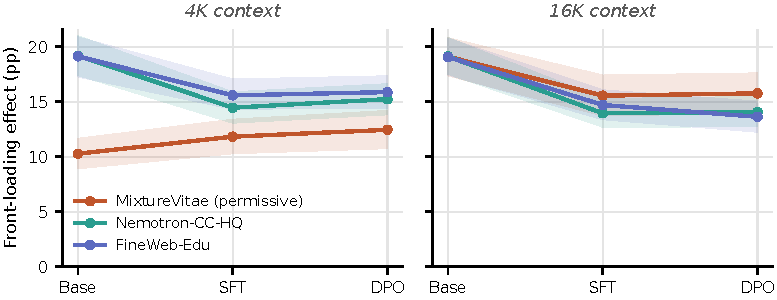
\includegraphics[width=\linewidth]{figures/frontloading_trajectory.pdf}
\caption{Front-loading effect on the reasoning suite average across post-training stages,
with 95\% paired item-level bootstrap intervals. Protocol~A.}
\label{fig:fl_trajectory}
\end{figure}

\begin{figure}[t]
\centering
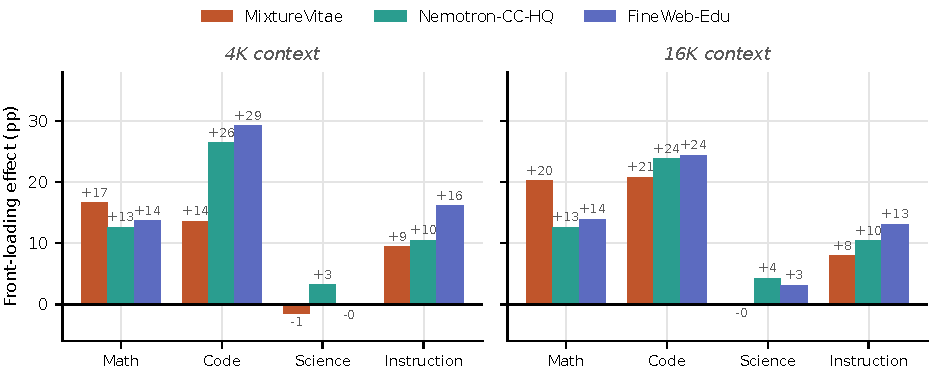
\includegraphics[width=\linewidth]{figures/frontloading_domains.pdf}
\caption{Front-loading effect by capability domain after Tulu3 SFT. The gain is broad
rather than confined to mathematics, and instruction following improves for every
substrate. Protocol~A.}
\label{fig:domains}
\end{figure}

\subsection{Reasoning post-training endpoints}
\label{app:phase2}

Table~\ref{tab:phase2_endpoints} gives the per-benchmark endpoints behind
Figure~\ref{fig:receptivity}, with each block's first row the starting checkpoint that the
OpenThoughts3-30K run was initialised from and re-evaluated under Protocol~B, so that
every comparison inside the table is paired. Table~\ref{tab:heldout_mv_grid} gives the
full held-out reasoning grid, four reasoning corpora applied from three starting
checkpoints with recipe, sample budget, and epoch count held fixed. Two observations that
the compact main-text version omits. Superior-Reasoning is a mixed control rather than a
failure, improving mathematics substantially while regressing code and instruction
following enough to lower the suite average from every starting point. And the DPO
starting point is the one that preserves instruction following through reasoning
post-training, ending at $43.0$ on IFEval against $45.0$ before the update, where the SFT
starting point falls to $25.6$.

% Generated by generate_workshop_artifacts.py. Do not edit by hand.
\begin{table}[t]
\centering
\caption{Reasoning post-training endpoints. Identical OpenThoughts3-30K post-training (30K samples, 5 epochs) is applied to every model, starting from the checkpoint named in each block's first row. Starting checkpoints are re-evaluated here, so these values are paired within the table and must not be compared against the Phase~1 tables. Protocol~B, the reasoning post-training protocol (Appendix Table~\ref{tab:eval-settings-B}). Single seed, so no error bars are available.}
\label{tab:phase2_endpoints}
\scriptsize
\setlength{\tabcolsep}{3pt}
\resizebox{\linewidth}{!}{%
\begin{tabular}{lrrrrrrrrrrrr}
\toprule
\textbf{Model} & \textbf{A24} & \textbf{A25} & \textbf{AMC} & \textbf{M500} & \textbf{GSM8K} & \textbf{HE} & \textbf{LCB} & \textbf{MBPP} & \textbf{GPQA} & \textbf{JEE} & \textbf{IFE} & \textbf{Avg} \\
\midrule
MV-16k (base) & 0.0 & 10.0 & 30.0 & 33.6 & 58.4 & 48.2 & 11.7 & 41.0 & 26.3 & 8.3 & 42.6 & 28.2 \\
\quad $\to$ SFT $\to$ OT30K & 20.0 & 16.7 & 29.8 & 72.8 & 52.5 & 58.5 & 10.0 & 29.2 & 36.4 & 4.6 & 25.6 & 32.4 \\
\quad $\to$ DPO $\to$ OT30K & 10.0 & 6.7 & 20.0 & 36.4 & 51.4 & 46.3 & 11.9 & 40.8 & 26.8 & 11.5 & 43.0 & 27.7 \\
\quad $\to$ OT30K \textbf{(no Phase 1)} & 20.0 & 16.7 & 25.0 & 71.4 & 58.9 & 57.3 & 10.0 & 31.6 & 26.3 & 6.0 & 26.6 & 31.8 \\
\midrule
FineWeb-Edu-16k $\to$ SFT & 0.0 & 0.0 & 2.5 & 1.4 & 8.5 & 2.4 & 0.3 & 2.2 & 30.3 & 3.0 & 27.6 & 7.1 \\
\quad $\to$ OT30K & 0.0 & 0.0 & 0.0 & 0.8 & 9.2 & 0.0 & 0.0 & 0.0 & 23.7 & 0.0 & 17.8 & 4.7 \\
\midrule
Nemotron-16k $\to$ SFT & 0.0 & 0.0 & 2.5 & 1.4 & 6.4 & 1.5 & 0.2 & 0.2 & 25.9 & 3.3 & 36.5 & 7.1 \\
\quad $\to$ OT30K & 0.0 & 0.0 & 0.0 & 0.4 & 5.3 & 0.0 & 0.0 & 0.2 & 21.2 & 0.2 & 20.0 & 4.3 \\
\midrule
Comma0.1-16k $\to$ SFT & 0.0 & 0.0 & 5.0 & 2.2 & 5.8 & 12.8 & 0.8 & 23.6 & 30.3 & 5.0 & 35.4 & 11.0 \\
\quad $\to$ OT30K & 0.0 & 0.0 & 0.0 & 1.6 & 14.0 & 1.8 & 0.0 & 0.0 & 28.8 & 0.0 & 20.0 & 6.0 \\
\midrule
SmolLM2-16k $\to$ SFT & 0.0 & 3.3 & 2.5 & 6.6 & 31.9 & 28.7 & 3.3 & 37.4 & 25.8 & 6.5 & 45.0 & 17.4 \\
\quad $\to$ OT30K & 0.0 & 0.0 & 0.0 & 14.0 & 26.3 & 23.2 & 0.5 & 15.8 & 27.3 & 3.3 & 34.0 & 13.1 \\
\midrule
Qwen2.5 $\to$ SFT & 0.0 & 0.0 & 7.5 & 19.6 & 39.7 & 48.2 & 3.8 & 44.6 & 22.7 & 7.5 & 44.4 & 21.6 \\
\quad $\to$ OT30K & 10.0 & 6.7 & 15.0 & 49.2 & 56.9 & 20.7 & 1.4 & 8.4 & 25.8 & 2.1 & 27.6 & 20.3 \\
\midrule
Qwen3 $\to$ SFT & 10.0 & 0.0 & 12.5 & 23.0 & 69.2 & 64.6 & 3.8 & 55.8 & 25.8 & 11.7 & 53.2 & 30.0 \\
\quad $\to$ OT30K & 0.0 & 0.0 & 0.0 & 10.6 & 29.0 & 7.3 & 1.1 & 10.6 & 28.3 & 0.5 & 30.4 & 10.7 \\
\bottomrule
\end{tabular}}
\end{table}


% Generated by generate_workshop_artifacts.py. Do not edit by hand.
\begin{table}[t]
\centering
\caption{Full held-out reasoning grid for MixtureVitae: four reasoning corpora applied from three starting checkpoints, with recipe, sample budget, and epoch count held fixed so that only the identity of the reasoning corpus changes. ``--'' marks a benchmark that was not evaluated, and that row's average is taken over the remaining ten. Protocol~B, the reasoning post-training protocol (Appendix Table~\ref{tab:eval-settings-B}). Single seed, so no error bars are available.}
\label{tab:heldout_mv_grid}
\scriptsize
\setlength{\tabcolsep}{3pt}
\resizebox{\linewidth}{!}{%
\begin{tabular}{lrrrrrrrrrrrr}
\toprule
\textbf{Reasoning corpus} & \textbf{A24} & \textbf{A25} & \textbf{AMC} & \textbf{M500} & \textbf{GSM8K} & \textbf{HE} & \textbf{LCB} & \textbf{MBPP} & \textbf{GPQA} & \textbf{JEE} & \textbf{IFE} & \textbf{Avg} \\
\midrule
\multicolumn{13}{l}{\emph{Starting from the post-YaRN base checkpoint}} \\
\quad \emph{starting checkpoint} & 0.0 & 10.0 & 30.0 & 33.6 & 58.6 & 48.2 & 11.7 & 41.0 & 26.3 & 8.3 & 42.6 & 28.2 \\
\quad OpenThoughts3 & 20.0 & 16.7 & 25.0 & 70.2 & 59.1 & 57.3 & 10.0 & 31.6 & 26.3 & 6.0 & 26.6 & 31.7~{\scriptsize($+3.5$)} \\
\quad AceReason & 3.3 & 13.3 & 30.0 & 69.2 & 61.8 & 52.4 & 9.8 & 35.6 & 26.3 & 10.4 & 24.6 & 30.6~{\scriptsize($+2.4$)} \\
\quad Nemotron-Cascade & 3.3 & 6.7 & 27.5 & 70.0 & 60.0 & 49.4 & 11.4 & 35.8 & 26.8 & 10.2 & 29.0 & 30.0~{\scriptsize($+1.8$)} \\
\quad Superior-Reasoning & 3.3 & 3.3 & 20.0 & 51.0 & 62.5 & 35.4 & 6.5 & 12.2 & 28.3 & 4.2 & 26.4 & 23.0~{\scriptsize($-5.2$)} \\
\midrule
\multicolumn{13}{l}{\emph{Starting from the Tulu3 SFT checkpoint}} \\
\quad \emph{starting checkpoint} & 0.0 & 0.0 & 5.0 & 35.2 & 51.0 & 45.1 & 8.1 & 40.2 & 28.3 & 6.5 & 41.8 & 23.8 \\
\quad OpenThoughts3 & 6.7 & 10.0 & 20.0 & 70.6 & 50.7 & 58.5 & 10.0 & 29.2 & 36.4 & 4.6 & 25.6 & 29.3~{\scriptsize($+5.5$)} \\
\quad AceReason & 3.3 & 20.0 & 25.0 & 69.4 & 54.4 & 48.2 & 10.8 & 33.6 & 27.3 & 9.9 & 25.6 & 29.8~{\scriptsize($+6.0$)} \\
\quad Nemotron-Cascade & 3.3 & 13.3 & 27.5 & 66.8 & 52.6 & 50.6 & -- & 32.8 & 34.8 & 7.3 & 30.6 & 32.0~{\scriptsize($+8.2$)} \\
\quad Superior-Reasoning & 6.7 & 3.3 & 20.0 & 51.6 & 55.6 & 22.0 & 6.2 & 15.6 & 25.8 & 4.9 & 27.0 & 21.7~{\scriptsize($-2.1$)} \\
\midrule
\multicolumn{13}{l}{\emph{Starting from the Tulu3 SFT + DPO checkpoint}} \\
\quad \emph{starting checkpoint} & 0.0 & 0.0 & 2.5 & 33.2 & 51.9 & 47.6 & 8.7 & 40.4 & 27.8 & 8.9 & 45.0 & 24.2 \\
\quad OpenThoughts3 & 10.0 & 6.7 & 20.0 & 36.4 & 50.7 & 44.5 & 11.9 & 40.8 & 26.8 & 11.5 & 43.0 & 27.5~{\scriptsize($+3.3$)} \\
\quad AceReason & 6.7 & 16.7 & 27.5 & 70.8 & 55.4 & 48.2 & 11.4 & 32.6 & 23.7 & 9.8 & 25.0 & 29.8~{\scriptsize($+5.6$)} \\
\quad Nemotron-Cascade & 6.7 & 10.0 & 25.0 & 68.2 & 53.5 & 50.0 & 13.3 & 34.8 & 28.8 & 9.7 & 30.4 & 30.0~{\scriptsize($+5.8$)} \\
\quad Superior-Reasoning & 3.3 & 6.7 & 20.0 & 54.2 & 55.1 & 28.7 & 5.7 & 13.2 & 24.7 & 5.3 & 28.0 & 22.3~{\scriptsize($-1.9$)} \\
\bottomrule
\end{tabular}}
\end{table}


\subsection{Mixture composition at a 100B budget}
\label{app:mixture100b}

Tables~\ref{tab:evalchemy_table1} and~\ref{tab:lang_eval_table1} give the per-benchmark
values behind the mixture-composition ablation of Section~\ref{sec:zoo}, in which two
ablated variants of the permissive mixture are pre-trained at 100B tokens and passed
through the same Phase 1 pipeline. Removing the instruction-and-reasoning subset collapses
performance across mathematics, code, and reasoning at both context lengths, with AIME24
and AIME25 at zero, MATH500 below three, and suite averages of $6.1$ to $8.5$ at 4K and
$6.7$ to $7.5$ at 16K, and Tulu3 SFT does not repair it. Removing the curated web subset
behaves very differently, reaching $18.6$ at the 4K base and $16.1$ to $17.5$ after Phase
1, never below the full mixture and above it on MATH500, AMC23, HumanEval, and MBPP. On
language understanding the web ablation costs about a point, $49.0$ to $50.0$ mean
accuracy against $50.0$ to $51.0$ for the full mixture, while the instruction ablation
costs 4 to 5 points that Phase 1 does not close. We state this for the scale and budget
tested and do not generalise it.

\subsection{Smaller scale check at 0.4B}
\label{app:smallscale}

Tables~\ref{tab:evalchemy_table4} and~\ref{tab:lang_eval_table4} compare a 0.4B permissive
model against Baguettotron, a 0.32B model trained on the PleIAs SYNTH
mix~\citep{synthpleias2025}, under the same Phase 1 pipeline. The permissive model reaches $12.1$ reasoning suite average after DPO against $6.2$ for Baguettotron, with HumanEval and
MBPP pass@1 of $15.3$ and $22.6$ against near zero, and $45.0$ against $42.0$ to $43.0$
mean accuracy on the language suite. The decontamination status of the SYNTH mix is
undocumented while our model is decontaminated against every benchmark reported here, so
some part of Baguettotron's score may reflect train and test overlap that we cannot rule
out from outside the release. This comparison is a sanity check on the direction of the
effect at a second scale and not a scaling result.


\begin{table}[ht]
\centering
\caption{Per-benchmark results for the 100B-token MixtureVitae mixture-composition ablation on the primary reasoning suite. Removing the instruction-and-reasoning subset causes a broad collapse in math, code, and reasoning that Phase 1 Tulu3 SFT/DPO does not recover, whereas removing the curated web subset leaves performance comparable to, and on several benchmarks stronger than, the full mixture at both 4K and 16K context. Bold marks the column maximum.}
\label{tab:evalchemy_table1}
\scriptsize
\resizebox{\columnwidth}{!}{%
\begin{tabular}{lrrrrrrrrrrrr}
\toprule
\textbf{Model} & \textbf{A24} & \textbf{A25} & \textbf{AMC} & \textbf{M500} & \textbf{GSM8K} & \textbf{HE} & \textbf{LCB} & \textbf{MBPP} & \textbf{GPQA} & \textbf{JEE} & \textbf{IFE} & \textbf{Avg} \\
\midrule
MV-noinstruct & 0.0 & 0.0 & 0.0 & 0.4 & 2.6 & 0.6 & 0.0 & 14.2 & 23.9 & 0.0 & 24.8 & 6.1 \\
\quad $\to$ SFT & 0.0 & 0.0 & 2.5 & 1.8 & 4.2 & 7.3 & 1.0 & 15.8 & 20.7 & 3.4 & 29.9 & 7.9 \\
\quad $\to$ SFT $\to$ DPO & 0.0 & 0.0 & 2.5 & 2.0 & 3.8 & 7.0 & 1.4 & 15.2 & 25.1 & 4.0 & 32.0 & 8.5 \\
\midrule
\addlinespace[0.3em]
MV-noinstruct-16k & 0.0 & 0.0 & 2.5 & 1.6 & 4.2 & 1.5 & 0.0 & 2.0 & 24.6 & 4.7 & 32.9 & 6.7 \\
\quad $\to$ SFT & 0.0 & 0.0 & 0.0 & 2.2 & 4.8 & 3.4 & 0.4 & 3.4 & \textbf{25.6} & 2.1 & 35.2 & 7.0 \\
\quad $\to$ SFT $\to$ DPO & 0.0 & 0.0 & 2.5 & 2.6 & 5.2 & 4.9 & 0.6 & 4.8 & 23.7 & 2.2 & 36.0 & 7.5 \\
\midrule
\addlinespace[0.3em]
MV-noweb & 0.0 & 0.0 & 17.5 & 26.4 & 42.4 & 23.5 & \textbf{7.4} & 34.6 & 23.7 & 2.6 & 26.5 & \textbf{18.6} \\
\quad $\to$ SFT & 0.0 & 0.0 & 7.5 & 10.0 & 36.0 & 23.6 & 2.4 & 36.8 & 22.4 & 3.7 & 35.0 & 16.1 \\
\quad $\to$ SFT $\to$ DPO & 0.0 & \textbf{3.3} & 10.0 & 12.2 & 36.5 & \textbf{25.1} & 1.8 & \textbf{38.0} & 25.2 & 4.3 & 36.2 & 17.5 \\
\midrule
\addlinespace[0.3em]
MV-noweb-16k & 0.0 & 0.0 & 10.0 & 35.0 & \textbf{44.7} & 10.7 & 3.5 & 9.0 & 23.9 & 4.4 & 37.4 & 16.2 \\
\quad $\to$ SFT & 0.0 & 0.0 & 7.5 & 18.2 & 33.6 & 9.5 & 3.5 & 7.2 & 22.1 & 4.3 & 38.2 & 13.1 \\
\quad $\to$ SFT $\to$ DPO & \textbf{3.3} & \textbf{3.3} & \textbf{20.0} & 21.2 & 35.0 & 11.0 & 3.3 & 7.8 & 21.0 & 2.9 & 38.3 & 15.2 \\
\midrule
\addlinespace[0.3em]
MV & \textbf{3.3} & 0.0 & 0.0 & 12.2 & 42.1 & 0.6 & 0.0 & 0.2 & 24.4 & 3.2 & 21.2 & 9.8 \\
\quad $\to$ SFT & 0.0 & 0.0 & 5.0 & 6.6 & 38.4 & 22.3 & 3.3 & 36.8 & 20.7 & 2.5 & 34.9 & 15.5 \\
\quad $\to$ SFT $\to$ DPO & 0.0 & 0.0 & 5.0 & 8.0 & 39.2 & 22.6 & 4.3 & 36.4 & 24.4 & 2.9 & 35.1 & 16.2 \\
\midrule
\addlinespace[0.3em]
MV-16k & 0.0 & 0.0 & 17.5 & \textbf{35.2} & 40.6 & 2.5 & 3.7 & 7.2 & 22.4 & \textbf{7.2} & 40.4 & 16.1 \\
\quad $\to$ SFT & 0.0 & 0.0 & 0.0 & 3.2 & 36.5 & 11.6 & 0.6 & 6.4 & 23.9 & 4.4 & 39.5 & 11.5 \\
\quad $\to$ SFT $\to$ DPO & 0.0 & 0.0 & 0.0 & 3.4 & 36.4 & 0.9 & 0.8 & 8.2 & 24.6 & 4.0 & \textbf{41.6} & 10.9 \\
\bottomrule
\end{tabular}
}
\end{table}


\begin{table}[ht]
\centering
\caption{Reasoning-suite comparison between decontaminated and non-decontaminated 300B MixtureVitae checkpoints at 4K and 16K context, before and after Phase 1 Tulu3 SFT/DPO. Decontamination changes some base scores, but the post-training picture remains the same: the gains reported in the main paper persist after decontamination. Bold marks the column maximum.}
\label{tab:evalchemy_table3}
\resizebox{\textwidth}{!}{%
\scriptsize
\begin{tabular}{llrrrrrrrrrrrr}
\toprule
\textbf{Base} & \textbf{Model} & \textbf{A24} & \textbf{A25} & \textbf{AMC} & \textbf{M500} & \textbf{GSM8K} & \textbf{HE} & \textbf{LCB} & \textbf{MBPP} & \textbf{GPQA} & \textbf{JEE} & \textbf{IFE} & \textbf{Avg}  \\
\midrule
\multirow{6}{*}{Not Decontaminated} & MV & 0.0 & 0.0 & 15.0 & 14.6 & 53.1 & 26.6 & 11.2 & 43.0 & 22.2 & 5.0 & 27.8 & 19.9 \\
 & \quad $\to$ SFT & \textbf{6.7} & 0.0 & 2.5 & 16.4 & 50.6 & 32.5 & 11.2 & 42.6 & 25.6 & 3.5 & 45.0 & 21.5 \\
 & \quad $\to$ SFT $\to$ DPO & 0.0 & 0.0 & 7.5 & 17.6 & 50.9 & 32.8 & 12.5 & 43.0 & \textbf{27.8} & 3.5 & 46.7 & 22.0 \\
\cmidrule{2-14}
 & MV-16k & 3.3 & 6.7 & 20.0 & 36.6 & \textbf{61.8} & 30.0 & 16.8 & 41.8 & 22.6 & \textbf{11.0} & 47.9 & 27.1 \\
 & \quad $\to$ SFT & 0.0 & 0.0 & 5.0 & 18.0 & 51.3 & 29.7 & 10.6 & \textbf{43.2} & 27.3 & 2.7 & 49.5 & 21.6 \\
 & \quad $\to$ SFT $\to$ DPO & 0.0 & 0.0 & 0.0 & 18.0 & 51.5 & 30.0 & 11.0 & 41.8 & 25.2 & 3.8 & \textbf{50.7} & 21.1 \\
\midrule
\addlinespace[0.3em]
\multirow{6}{*}{Decontaminated} & MV & 0.0 & \textbf{10.0} & 7.5 & 17.4 & 53.5 & 11.7 & 12.7 & 18.6 & 23.9 & 4.1 & 25.6 & 16.8 \\
 & \quad $\to$ SFT & 0.0 & 0.0 & 7.5 & 28.6 & 49.3 & 27.9 & 2.1 & 41.2 & 26.1 & 4.2 & 42.4 & 20.8 \\
 & \quad $\to$ SFT $\to$ DPO & 0.0 & 0.0 & 15.0 & 27.4 & 50.5 & 27.9 & 1.8 & 40.8 & 24.6 & 3.1 & 42.9 & 21.3 \\
\cmidrule{2-14}
 & MV-16k & 0.0 & 0.0 & \textbf{27.5} & \textbf{46.0} & 58.6 & 31.9 & \textbf{22.7} & 39.8 & 25.2 & 8.2 & 46.9 & \textbf{27.9} \\
 & \quad $\to$ SFT & 3.3 & 0.0 & 12.5 & 31.0 & 51.9 & \textbf{33.2} & 15.5 & 40.6 & 23.4 & 5.2 & 47.1 & 24.0 \\
 & \quad $\to$ SFT $\to$ DPO & \textbf{6.7} & 0.0 & 15.0 & 33.6 & 52.1 & \textbf{33.2} & 14.9 & 40.0 & 25.2 & 5.4 & 49.5 & 25.0 \\
\bottomrule
\end{tabular}
}
\end{table}


\begin{table}[ht]
\centering
\caption{Reasoning-suite results for the smaller-scale comparison between MV (0.4B) and Baguettotron. Across 4K and 16K context, MV is substantially more receptive to Phase 1 post-training, especially on code and broader reasoning, while Baguettotron remains weak throughout. Bold marks the column maximum.}
\label{tab:evalchemy_table4}
\scriptsize
\resizebox{\columnwidth}{!}{%
\begin{tabular}{lrrrrrrrrrrrr}
\toprule
\textbf{Model} & \textbf{A24} & \textbf{A25} & \textbf{AMC} & \textbf{M500} & \textbf{GSM8K} & \textbf{HE} & \textbf{LCB} & \textbf{MBPP} & \textbf{GPQA} & \textbf{JEE} & \textbf{IFE} & \textbf{Avg} \\
\midrule
Baguettotron & 0.0 & \textbf{0.0} & 0.0 & 0.2 & 2.3 & 0.0 & 0.0 & 0.0 & 23.1 & 0.2 & 24.3 & 4.5 \\
\quad $\to$ SFT & 0.0 & \textbf{0.0} & 2.5 & 2.0 & 7.7 & 0.0 & 0.0 & 0.0 & 24.4 & 1.3 & 26.9 & 5.9 \\
\quad $\to$ SFT $\to$ DPO & 0.0 & \textbf{0.0} & 0.0 & 2.8 & 8.3 & 0.0 & 0.0 & 0.0 & \textbf{26.3} & 1.1 & 30.2 & 6.2 \\
\midrule
\addlinespace[0.3em]
Baguettotron 16k & 0.0 & \textbf{0.0} & 0.0 & 2.0 & 5.2 & 0.6 & 0.0 & 0.0 & 21.6 & 1.8 & \textbf{34.2} & 5.9 \\
\quad $\to$ SFT & 0.0 & \textbf{0.0} & 2.5 & 2.4 & 8.1 & 0.0 & 0.0 & 0.0 & 24.4 & 1.1 & 30.0 & 6.2 \\
\quad $\to$ SFT $\to$ DPO & 0.0 & \textbf{0.0} & 2.5 & 3.2 & 8.7 & 0.0 & 0.0 & 0.0 & 24.9 & 1.5 & 31.8 & 6.6 \\
\midrule
\addlinespace[0.3em]
MV (0.4B) & \textbf{3.3} & \textbf{0.0} & 2.5 & 0.6 & 28.7 & 1.2 & 1.0 & 5.2 & 22.4 & 1.1 & 19.6 & 7.8 \\
\quad $\to$ SFT & 0.0 & \textbf{0.0} & 2.5 & 6.2 & 23.1 & 0.6 & 7.0 & 12.2 & 25.6 & 1.7 & 27.1 & 9.6 \\
\quad $\to$ SFT $\to$ DPO & 0.0 & \textbf{0.0} & 2.5 & 7.4 & 23.1 & \textbf{15.3} & \textbf{8.2} & \textbf{22.6} & 24.1 & 2.3 & 28.1 & 12.1 \\
\midrule
\addlinespace[0.3em]
MV-16k (0.4B) & 0.0 & \textbf{0.0} & \textbf{7.5} & \textbf{19.8} & \textbf{29.5} & 6.4 & 0.8 & 13.8 & 22.2 & \textbf{4.3} & 32.6 & \textbf{12.4} \\
\quad $\to$ SFT & 0.0 & \textbf{0.0} & 2.5 & 6.2 & 24.5 & 8.9 & 1.4 & 13.6 & 22.9 & 2.3 & 29.9 & 10.2 \\
\quad $\to$ SFT $\to$ DPO & 0.0 & \textbf{0.0} & 2.5 & 6.8 & 24.9 & 7.7 & 1.6 & 11.2 & 23.1 & 2.6 & 31.4 & 10.1 \\
\bottomrule
\end{tabular}}

\end{table}


\begin{table}[htbp]
\centering
\caption{Per-benchmark results for the 100B token MixtureVitae mixture composition ablation on the standard language understanding suite. Removing the instruction and reasoning subset creates a persistent language gap that Phase 1 does not close, whereas removing the curated web subset leaves language performance close to the full mixture across stages and both context lengths. Bold marks the column maximum.}
\label{tab:lang_eval_table1}
\scriptsize
\resizebox{\columnwidth}{!}{%
\begin{tabular}{lrrrrrrrrrrrr}
\toprule
\textbf{Model} & \textbf{ARC-C} & \textbf{ARC-E} & \textbf{BoolQ} & \textbf{CSQA} & \textbf{COPA} & \textbf{HellaS} & \textbf{LAMBADA} & \textbf{MMLU} & \textbf{OBQA} & \textbf{PIQA} & \textbf{WinoG} & \textbf{Avg} \\
\midrule
MV-noinstruct & 32.0 & 61.0 & 58.0 & 18.0 & 66.0 & 46.0 & 46.0 & 25.0 & 33.0 & 68.0 & 55.0 & 46.0 \\
\quad $\to$SFT & 32.0 & 61.0 & 57.0 & 19.0 & 66.0 & 46.0 & \textbf{47.0} & 25.0 & 33.0 & 68.0 & 55.0 & 46.0 \\
\quad $\to$SFT $\to$DPO & 32.0 & 61.0 & 57.0 & 19.0 & 66.0 & 47.0 & \textbf{47.0} & 25.0 & 33.0 & 68.0 & 55.0 & 46.0 \\
\midrule
\addlinespace[0.3em]
MV-noinstruct-16k & 33.0 & 60.0 & 63.0 & 19.0 & 69.0 & 46.0 & \textbf{47.0} & 25.0 & 33.0 & 67.0 & 55.0 & 47.0 \\
\quad $\to$SFT & 31.0 & 60.0 & 61.0 & 18.0 & 67.0 & 46.0 & \textbf{47.0} & 25.0 & 33.0 & 67.0 & 56.0 & 46.0 \\
\quad $\to$SFT $\to$DPO & 31.0 & 60.0 & 61.0 & 18.0 & 67.0 & 47.0 & \textbf{47.0} & 25.0 & 32.0 & 67.0 & 56.0 & 46.0 \\
\midrule
\addlinespace[0.3em]
MV-noweb & 34.0 & \textbf{65.0} & 67.0 & 35.0 & 67.0 & 46.0 & 39.0 & 31.0 & 33.0 & 68.0 & 56.0 & 49.0 \\
\quad $\to$SFT & 33.0 & 63.0 & 65.0 & 35.0 & 69.0 & 47.0 & 41.0 & \textbf{33.0} & 32.0 & 67.0 & 55.0 & 49.0 \\
\quad $\to$SFT $\to$DPO & 33.0 & 63.0 & 65.0 & 35.0 & 69.0 & 47.0 & 41.0 & \textbf{33.0} & 32.0 & 67.0 & 55.0 & 49.0 \\
\midrule
\addlinespace[0.3em]
MV-noweb-16k & \textbf{36.0} & \textbf{65.0} & 70.0 & \textbf{37.0} & \textbf{70.0} & 45.0 & 40.0 & 32.0 & 32.0 & 67.0 & 56.0 & 50.0 \\
\quad $\to$SFT & 33.0 & 63.0 & 66.0 & 34.0 & 69.0 & 46.0 & 41.0 & \textbf{33.0} & 33.0 & 67.0 & 56.0 & 49.0 \\
\quad $\to$SFT $\to$DPO & 33.0 & 63.0 & 67.0 & 34.0 & 69.0 & 47.0 & 41.0 & \textbf{33.0} & 33.0 & 67.0 & 56.0 & 49.0 \\
\midrule
\addlinespace[0.3em]
MV & 34.0 & \textbf{65.0} & \textbf{71.0} & 31.0 & 67.0 & 48.0 & 44.0 & 32.0 & \textbf{34.0} & 68.0 & 58.0 & 50.0 \\
\quad $\to$SFT & 34.0 & 64.0 & \textbf{71.0} & 32.0 & 69.0 & \textbf{49.0} & 45.0 & \textbf{33.0} & \textbf{34.0} & \textbf{69.0} & 58.0 & \textbf{51.0} \\
\quad $\to$SFT $\to$DPO & 34.0 & 64.0 & \textbf{71.0} & 32.0 & \textbf{70.0} & \textbf{49.0} & 45.0 & \textbf{33.0} & 33.0 & \textbf{69.0} & 58.0 & \textbf{51.0} \\
\midrule
\addlinespace[0.3em]
MV-16k & 35.0 & \textbf{65.0} & 68.0 & 30.0 & 67.0 & 47.0 & 45.0 & \textbf{33.0} & 33.0 & 68.0 & 57.0 & 50.0 \\
\quad $\to$SFT & 33.0 & 64.0 & 69.0 & 29.0 & 68.0 & \textbf{49.0} & 45.0 & 32.0 & 33.0 & 68.0 & \textbf{59.0} & 50.0 \\
\quad $\to$SFT $\to$DPO & 33.0 & 64.0 & 69.0 & 30.0 & 68.0 & \textbf{49.0} & 45.0 & 32.0 & 33.0 & 68.0 & \textbf{59.0} & 50.0 \\
\bottomrule
\end{tabular}
}
\end{table}


\begin{table}[htbp]
\centering
\caption{Full language suite results for the main 1.7B comparison. Phase 1 Tulu3 SFT/DPO leaves language scores largely unchanged, with MixtureVitae matching FineWeb-Edu, trailing Nemotron, and remaining below the more heavily pretrained external baselines. Bold marks the column maximum.}
\label{tab:lang_eval_table2}
\resizebox{\textwidth}{!}{%
\scriptsize
\begin{tabular}{lrrrrrrrrrrrr}
\toprule
Model & ARC-C & ARC-E & BoolQ & CSQA & COPA & HellaS & LAMBADA & MMLU & OBQA & PIQA & WinoG & Avg  \\
\midrule
Comma0.1-300BT       & 36.0 & 63.0 & 62.0 & 21.0 & 71.0 & 53.0 & 54.0 & 27.0 & 33.0 & 71.0 & 60.0 & 50.0 \\
\quad $\to$SFT & 37.0 & 65.0 & 64.0 & 20.0 & 74.0 & 54.0 & 57.0 & 27.0 & 33.0 & 72.0 & 61.0 & 51.0 \\
\quad $\to$SFT $\to$DPO & 37.0 & 65.0 & 65.0 & 20.0 & 74.0 & 54.0 & 57.0 & 27.0 & 33.0 & 72.0 & 61.0 & 51.0 \\
\midrule
\addlinespace[0.3em]
MV          & 40.0 & 71.0 & 74.0 & 51.0 & 71.0 & 54.0 & 48.0 & 42.0 & 34.0 & 70.0 & 58.0 & 56.0 \\
\quad $\to$SFT & 39.0 & 70.0 & 73.0 & 50.0 & 70.0 & 56.0 & 50.0 & 43.0 & 34.0 & 70.0 & 58.0 & 56.0 \\
\quad $\to$SFT $\to$DPO & 39.0 & 70.0 & 73.0 & 50.0 & 71.0 & 56.0 & 50.0 & 43.0 & 34.0 & 70.0 & 58.0 & 56.0 \\
\midrule
\addlinespace[0.3em]
MV-16k          & 42.0 & 71.0 & 73.0 & 49.0 & 67.0 & 53.0 & 49.0 & 41.0 & 32.0 & 70.0 & 58.0 & 55.0 \\
\quad $\to$SFT & 39.0 & 70.0 & 73.0 & 50.0 & 69.0 & 55.0 & 50.0 & 42.0 & 34.0 & 70.0 & 57.0 & 55.0 \\
\quad $\to$SFT $\to$DPO & 39.0 & 71.0 & 73.0 & 50.0 & 69.0 & 55.0 & 50.0 & 42.0 & 34.0 & 70.0 & 57.0 & 55.0 \\
\midrule
\addlinespace[0.3em]
Qwen2.5-1.5B       & \textbf{54.0} & 81.0 & 78.0 & 76.0 & 83.0 & 68.0 & 62.0 & 61.0 & 40.0 & 77.0 & 63.0 & \textbf{68.0} \\
\quad $\to$SFT & 51.0 & 79.0 & 70.0 & \textbf{77.0} & 82.0 & 68.0 & 60.0 & 60.0 & 40.0 & 77.0 & 63.0 & 66.0 \\
\quad $\to$SFT $\to$DPO & 52.0 & 79.0 & 70.0 & 76.0 & 82.0 & 68.0 & 60.0 & 60.0 & 39.0 & 77.0 & 63.0 & 66.0 \\
\midrule
\addlinespace[0.3em]
Qwen3-1.7B       & \textbf{54.0} & \textbf{82.0} & \textbf{83.0} & 76.0 & 82.0 & 67.0 & 63.0 & \textbf{63.0} & 38.0 & 76.0 & 64.0 & \textbf{68.0} \\
\quad $\to$SFT & 53.0 & 81.0 & 82.0 & \textbf{77.0} & 80.0 & 68.0 & 61.0 & \textbf{63.0} & 39.0 & 76.0 & 64.0 & \textbf{68.0} \\
\quad $\to$SFT $\to$DPO & 53.0 & 81.0 & \textbf{83.0} & \textbf{77.0} & 80.0 & 68.0 & 61.0 & \textbf{63.0} & 39.0 & 76.0 & 64.0 & \textbf{68.0} \\
\midrule
\addlinespace[0.3em]
SmolLM2-1.7B       & \textbf{54.0} & 80.0 & 75.0 & 60.0 & 82.0 & 73.0 & 67.0 & 50.0 & \textbf{44.0} & \textbf{79.0} & \textbf{67.0} & 66.0 \\
\quad $\to$SFT & 53.0 & 80.0 & 75.0 & 61.0 & \textbf{85.0} & \textbf{74.0} & \textbf{69.0} & 49.0 & 43.0 & \textbf{79.0} & \textbf{67.0} & 67.0 \\
\quad $\to$SFT $\to$DPO & \textbf{54.0} & 80.0 & 75.0 & 61.0 & \textbf{85.0} & \textbf{74.0} & \textbf{69.0} & 49.0 & 43.0 & \textbf{79.0} & \textbf{67.0} & 67.0 \\
\midrule
\addlinespace[0.3em]
FineWeb-Edu-300BT & 48.0 & 77.0 & 65.0 & 21.0 & 82.0 & 67.0 & 56.0 & 26.0 & 42.0 & 77.0 & 62.0 & 57.0 \\
\quad $\to$SFT & 48.0 & 79.0 & 66.0 & 20.0 & 83.0 & 68.0 & 59.0 & 27.0 & 42.0 & 77.0 & 63.0 & 57.0 \\
\quad $\to$SFT $\to$DPO & 48.0 & 78.0 & 66.0 & 20.0 & 83.0 & 68.0 & 59.0 & 27.0 & 42.0 & 77.0 & 63.0 & 57.0 \\
\midrule
\addlinespace[0.3em]
Nemotron       & 52.0 & 81.0 & 77.0 & 49.0 & \textbf{85.0} & 71.0 & 58.0 & 46.0 & 42.0 & \textbf{79.0} & 65.0 & 64.0 \\
\quad $\to$SFT & 48.0 & 79.0 & 74.0 & 46.0 & 82.0 & 70.0 & 58.0 & 43.0 & 43.0 & 78.0 & 65.0 & 62.0 \\
\quad $\to$SFT $\to$DPO & 48.0 & 79.0 & 74.0 & 46.0 & 82.0 & 71.0 & 59.0 & 43.0 & 43.0 & 78.0 & 65.0 & 63.0 \\
\midrule
\bottomrule
\end{tabular}%
}
\end{table}


\begin{table}[htbp]
\centering
\caption{Language suite comparison between decontaminated and non-decontaminated 300B MixtureVitae checkpoints at 4K and 16K context, before and after Phase 1 Tulu3 SFT/DPO. In contrast to the reasoning suite, the language results are essentially unchanged by decontamination. Bold marks the column maximum.}
\label{tab:lang_eval_table3}
\scriptsize
\resizebox{\textwidth}{!}{%
\begin{tabular}{llrrrrrrrrrrrr}
\toprule
\textbf{Base} & \textbf{Model} & \textbf{ARC-C} & \textbf{ARC-E} & \textbf{BoolQ} & \textbf{CSQA} & \textbf{COPA} & \textbf{HellaS} & \textbf{LAMBADA} & \textbf{MMLU} & \textbf{OBQA} & \textbf{PIQA} & \textbf{WinoG} & \textbf{Avg} \\
\midrule
\multirow{6}{*}{Not Decontaminated} & MV & 40.0 & \textbf{71.0} & \textbf{75.0} & 49.0 & \textbf{73.0} & 54.0 & 48.0 & 38.0 & 35.0 & 70.0 & 58.0 & \textbf{56.0} \\
 & \quad $\to$SFT & 39.0 & 70.0 & \textbf{75.0} & 47.0 & 71.0 & 55.0 & \textbf{50.0} & 40.0 & 35.0 & 70.0 & 58.0 & 55.0 \\
 & \quad $\to$SFT $\to$DPO & 39.0 & 70.0 & \textbf{75.0} & 47.0 & 71.0 & 55.0 & \textbf{50.0} & 40.0 & 35.0 & 70.0 & 58.0 & \textbf{56.0} \\
\cmidrule{2-14}
 & MV-16k & 39.0 & \textbf{71.0} & \textbf{75.0} & 50.0 & 72.0 & 54.0 & 49.0 & 38.0 & \textbf{36.0} & \textbf{71.0} & 58.0 & \textbf{56.0} \\
 & \quad $\to$SFT & 39.0 & \textbf{71.0} & 74.0 & 48.0 & 72.0 & 55.0 & \textbf{50.0} & 38.0 & 35.0 & 70.0 & \textbf{59.0} & 55.0 \\
 & \quad $\to$SFT $\to$DPO & 39.0 & \textbf{71.0} & 74.0 & 48.0 & 72.0 & 55.0 & \textbf{50.0} & 38.0 & 35.0 & \textbf{71.0} & \textbf{59.0} & \textbf{56.0} \\
\midrule
\addlinespace[0.3em]
\multirow{6}{*}{Decontaminated} & MV & 40.0 & \textbf{71.0} & 74.0 & \textbf{51.0} & 71.0 & 54.0 & 48.0 & 42.0 & 34.0 & 70.0 & 58.0 & \textbf{56.0} \\
 & \quad $\to$SFT & 39.0 & 70.0 & 73.0 & 50.0 & 70.0 & \textbf{56.0} & \textbf{50.0} & \textbf{43.0} & 34.0 & 70.0 & 58.0 & \textbf{56.0} \\
 & \quad $\to$SFT $\to$DPO & 39.0 & 70.0 & 73.0 & 50.0 & 71.0 & \textbf{56.0} & \textbf{50.0} & \textbf{43.0} & 34.0 & 70.0 & 58.0 & \textbf{56.0} \\
\cmidrule{2-14}
 & MV-16k & \textbf{42.0} & \textbf{71.0} & 73.0 & 49.0 & 67.0 & 53.0 & 49.0 & 41.0 & 32.0 & 70.0 & 58.0 & 55.0 \\
 & \quad $\to$SFT & 39.0 & 70.0 & 73.0 & 50.0 & 69.0 & 55.0 & \textbf{50.0} & 42.0 & 34.0 & 70.0 & 57.0 & 55.0 \\
 & \quad $\to$SFT $\to$DPO & 39.0 & \textbf{71.0} & 73.0 & 50.0 & 69.0 & 55.0 & \textbf{50.0} & 42.0 & 34.0 & 70.0 & 57.0 & 55.0 \\
\bottomrule
\end{tabular}%
}
\end{table}


\begin{table}[htbp]
\centering
\caption{Language suite results for the smaller scale comparison between MV (0.4B) and Baguettotron. MV retains a small but consistent advantage across both context lengths and post-training stages, showing that its broader general-purpose edge at small scale is not limited to reasoning tasks. Bold marks the column maximum.}
\label{tab:lang_eval_table4}
\scriptsize
\resizebox{\columnwidth}{!}{%
\begin{tabular}{lrrrrrrrrrrrr}
\toprule
\textbf{Model} & \textbf{ARC-C} & \textbf{ARC-E} & \textbf{BoolQ} & \textbf{CSQA} & \textbf{COPA} & \textbf{HellaS} & \textbf{LAMBADA} & \textbf{MMLU} & \textbf{OBQA} & \textbf{PIQA} & \textbf{WinoG} & \textbf{Avg} \\
\midrule
Baguettotron & \textbf{33.0} & 58.0 & 61.0 & 19.0 & 56.0 & 36.0 & 30.0 & 27.0 & 31.0 & 61.0 & 53.0 & 42.0 \\
\quad $\to$SFT & 30.0 & 57.0 & 61.0 & 21.0 & 61.0 & 36.0 & 33.0 & 26.0 & \textbf{32.0} & 61.0 & \textbf{55.0} & 43.0 \\
\quad $\to$SFT $\to$DPO & 31.0 & 57.0 & 62.0 & 21.0 & 61.0 & 36.0 & 33.0 & 26.0 & \textbf{32.0} & 61.0 & 54.0 & 43.0 \\
\midrule
\addlinespace[0.3em]
Baguettotron 16k & 32.0 & 58.0 & 57.0 & 21.0 & 60.0 & 36.0 & 34.0 & 26.0 & 31.0 & 61.0 & \textbf{55.0} & 43.0 \\
\quad $\to$SFT & 31.0 & 57.0 & \textbf{64.0} & 20.0 & 61.0 & 36.0 & 33.0 & 26.0 & 31.0 & 61.0 & 54.0 & 43.0 \\
\quad $\to$SFT $\to$DPO & 31.0 & 57.0 & \textbf{64.0} & 19.0 & 61.0 & 36.0 & 33.0 & 26.0 & \textbf{32.0} & 61.0 & 54.0 & 43.0 \\
\midrule
\addlinespace[0.3em]
MV (0.4B) & 32.0 & \textbf{61.0} & 60.0 & \textbf{26.0} & 63.0 & \textbf{42.0} & 38.0 & 28.0 & 31.0 & \textbf{66.0} & 53.0 & \textbf{45.0} \\
\quad $\to$SFT & 29.0 & 59.0 & 50.0 & 25.0 & 63.0 & \textbf{42.0} & 40.0 & \textbf{29.0} & 30.0 & 65.0 & 53.0 & 44.0 \\
\quad $\to$SFT $\to$DPO & 29.0 & 59.0 & 50.0 & \textbf{26.0} & 63.0 & \textbf{42.0} & 40.0 & \textbf{29.0} & 30.0 & 65.0 & 54.0 & 44.0 \\
\midrule
\addlinespace[0.3em]
MV-16k (0.4B) & 32.0 & \textbf{61.0} & 58.0 & \textbf{26.0} & 63.0 & 41.0 & \textbf{41.0} & 28.0 & \textbf{32.0} & 65.0 & 54.0 & \textbf{45.0} \\
\quad $\to$SFT & 28.0 & 59.0 & 53.0 & 25.0 & \textbf{64.0} & \textbf{42.0} & 40.0 & \textbf{29.0} & 31.0 & 65.0 & \textbf{55.0} & \textbf{45.0} \\
\quad $\to$SFT $\to$DPO & 28.0 & 59.0 & 54.0 & 25.0 & 63.0 & \textbf{42.0} & \textbf{41.0} & \textbf{29.0} & 31.0 & 65.0 & \textbf{55.0} & \textbf{45.0} \\
\bottomrule
\end{tabular}
}
\end{table}

\begin{table}[htbp]
\centering
\caption{Language suite results after Phase 2 OpenThoughts3 30K post-training for the models evaluated in the OT3 experiments. Reasoning post-training preserves general language understanding, and MV-16K performs equally well with the full pipeline or with direct OT3 post-training from the post-YaRN base. Bold marks the column maximum.}
\label{tab:lang_eval_ot3_phase2}
\resizebox{\textwidth}{!}{%
\scriptsize
\begin{tabular}{lrrrrrrrrrrrr}
\toprule
\textbf{Model} & ARC-C & ARC-E & BoolQ & CSQA & COPA & HellaS & LAMBADA & MMLU & OBQA & PIQA & WinoG & Avg  \\
\midrule
MV-16k & & & & & & & & & & & &  \\
\quad $\to$SFT $\to$DPO $\to$OT30K                  & 40.0 & 70.0 & 73.0 & 50.0 & 71.0 & 55.0 & 49.0 & 41.0 & 34.0 & 70.0 & 59.0 & 56.0 \\
\quad $\to$OT30K (\textbf{no Phase 1})        & 43.0 & 71.0 & 74.0 & 49.0 & 69.0 & 54.0 & 49.0 & 42.0 & 33.0 & 70.0 & 59.0 & 56.0 \\
\midrule
\addlinespace[0.3em]
Comma-16k & & & & & & & & & & & &  \\
\quad $\to$SFT $\to$OT30K                        & 38.0 & 66.0 & 66.0 & 22.0 & 71.0 & 54.0 & 54.0 & 28.0 & 34.0 & 71.0 & 61.0 & 51.0 \\
\quad $\to$SFT $\to$DPO $\to$OT30K                  & 36.0 & 66.0 & 65.0 & 22.0 & 73.0 & 51.0 & 49.0 & 28.0 & 33.0 & 70.0 & 59.0 & 50.0 \\
\midrule
\addlinespace[0.3em]
FineWeb-Edu-16k & & & & & & & & & & & &  \\
\quad $\to$SFT $\to$OT30K                        & 47.0 & 79.0 & 70.0 & 21.0 & 83.0 & 67.0 & 54.0 & 27.0 & 41.0 & 77.0 & 63.0 & 57.0 \\
\midrule
\addlinespace[0.3em]
Nemotron-16k & & & & & & & & & & & &  \\
\quad $\to$SFT $\to$OT30K                        & 48.0 & 79.0 & 75.0 & 46.0 & 81.0 & 70.0 & 57.0 & 41.0 & 42.0 & \textbf{78.0} & 64.0 & 62.0 \\
\quad $\to$SFT $\to$DPO $\to$OT30K                  & 48.0 & 79.0 & 75.0 & 47.0 & 81.0 & 70.0 & 57.0 & 41.0 & 42.0 & \textbf{78.0} & 65.0 & 62.0 \\
\midrule
\addlinespace[0.3em]
Qwen2.5-1.5B & & & & & & & & & & & &  \\
\quad $\to$SFT $\to$OT30K                        & 51.0 & 78.0 & \textbf{77.0} & \textbf{73.0} & 84.0 & 67.0 & 46.0 & \textbf{59.0} & 41.0 & 77.0 & 63.0 & \textbf{65.0} \\
\quad $\to$SFT $\to$DPO $\to$OT30K                  & 51.0 & 78.0 & \textbf{77.0} & \textbf{73.0} & 84.0 & 67.0 & 46.0 & \textbf{59.0} & 41.0 & 77.0 & 63.0 & \textbf{65.0} \\
\midrule
\addlinespace[0.3em]
Qwen3-1.7B & & & & & & & & & & & &  \\
\quad $\to$SFT $\to$OT30K                        & 49.0 & 76.0 & 75.0 & 65.0 & 81.0 & 59.0 & 43.0 & 53.0 & 39.0 & 74.0 & 60.0 & 61.0 \\
\quad $\to$SFT $\to$DPO $\to$OT30K                  & 49.0 & 76.0 & 75.0 & 65.0 & 81.0 & 59.0 & 43.0 & 53.0 & 39.0 & 74.0 & 61.0 & 61.0 \\
\midrule
\addlinespace[0.3em]
SmolLM2-1.7B-16k & & & & & & & & & & & &  \\
\quad $\to$SFT $\to$OT30K                        & \textbf{53.0} & \textbf{81.0} & 70.0 & 59.0 & \textbf{88.0} & \textbf{71.0} & \textbf{64.0} & 44.0 & 43.0 & \textbf{78.0} & \textbf{66.0} & \textbf{65.0} \\
SmolLM2-1.7B-Instruct-16k & & & & & & & & & & & &  \\
\quad $\to$OT30K                              & 51.0 & 79.0 & 76.0 & 62.0 & 83.0 & \textbf{71.0} & 59.0 & 47.0 & \textbf{44.0} & \textbf{78.0} & \textbf{66.0} & \textbf{65.0} \\
\bottomrule
\end{tabular}%
}
\end{table}





\section{Experimental setup details}
\label{appendix:exp_details}

\subsection{\texttt{open-sci-ref} setup and hyperparameters}
\label{app:hyperparams}

\begin{table}[htbp]
\centering
\caption{The training schedules used in our experiments.}
\label{tab:training_schedules}
\renewcommand{\arraystretch}{1.5}
\begin{tabular}{@{}l c c c c c@{}}
\toprule
\textbf{Tokens} &
\textbf{\makecell[c]{Global Batch Size \\ (tokens)}} &
\textbf{Iterations} &
\textbf{\makecell[c]{Learning \\ Rate}} &
\textbf{Warmup} &
\textbf{\makecell[c]{Cooldown \\ (20\%)}} \\
\midrule
100B  & 4.12M & 23,842  & $4\times10^{-3}$ & 8,334  & 4,768  \\
300B & 4.12M & 72,661  & $4\times10^{-3}$ & 25,000 & 14,532 \\
\bottomrule
\end{tabular}

\end{table}


\begin{table*}[htbp]
\centering
\caption{\textbf{open-sci-ref}~\citep{nezhurina2025opensciref} model architecture and scales. We used tied embedding weights in all experiments.}
\label{tab:opensciref_scales}

\renewcommand{\arraystretch}{1.5}
\begin{tabular}{@{}l c c c c c c@{}}
\toprule
\textbf{\makecell[l]{Parameters (B) \\ (Non-Emb + Emb)}} &
\textbf{Layers} &
\textbf{Hidden} &
\textbf{Heads} &
\textbf{\makecell[l]{FFN \\ Hidden}} &
\textbf{Memory} &
\textbf{\makecell[l]{FLOPs}} \\
\midrule
$0.35 + 0.05 = 0.40$ & 22 & 1024 & 16 & 3840 & $2.88\,\mathrm{GB}$ & $2.4\times10^{9}$ \\
$1.61 + 0.10 = 1.71$ & 24 & 2048 & 32 & 8192 & $9.884\,\mathrm{GB}$ & $1.0\times10^{10}$ \\
\bottomrule
\end{tabular}
\end{table*}


This appendix details the exact model architectures and training hyperparameters used for all \texttt{open-sci-ref}-based pre-training. 

\paragraph{Model Architecture}
Table~\ref{tab:opensciref_scales} defines the two model scales used in our study. The columns are defined as follows:

\begin{description}
    \item[Parameters (B) (Non-Emb + Emb)] The total model parameters in billions, separated into \textbf{Non-Embedding} (Non-Emb) parameters (the core transformer blocks) and \textbf{Embedding} (Emb) parameters (the token lookup tables). As noted in the caption, we used tied embedding weights.
    \item[Layers] The total number of transformer blocks stacked in the model.
    \item[Hidden] The hidden size (or embedding dimension, $d_{\text{model}}$) of the model.
    \item[Heads] The number of attention heads in the multi-head attention mechanism.
    \item[FFN Hidden] The inner dimension of the Feed-Forward Network (FFN) layer within each transformer block.
    \item[Memory] The approximate VRAM required to store the model weights, in bfloat16.
    \item[FLOPs] An approximation of the training compute cost using the  \textbf{6N} rule: a standard estimate for a transformer's forward-and-backward pass, where \textbf{N} is the number of \textit{non-embedding} parameters~\citep{kaplan2020scalinglawsneurallanguage}.
\end{description}

\begin{table}[htbp]
\centering
\caption{Hyperparameters used for OT3 (OpenThoughts-3, 30k samples) SFT runs.
All runs share the same recipe, and only the attention backend and chat template change per architecture.}
\label{tab:ot30k_sft_hyperparams}
\begin{tabular}{ll}
\toprule
Hyperparameter & Value \\
\midrule
Dataset                       & \texttt{open-thoughts/OpenThoughts-3} (30k samples) \\
Stage / fine-tuning type      & SFT, full-parameter \\
Trainer / framework           & LLaMA-Factory \\
Distributed strategy          & DeepSpeed ZeRO-3 \\
Precision                     & BF16 \\
Liger Kernel                  & enabled \\
Attention backend             & FA2 (Llama/Qwen) / SDPA (opensci-arch) \\
\addlinespace
Sequence length (cutoff\_len) & 16{,}384 \\
Per-device batch size         & 1 \\
Gradient accumulation steps   & 4 \\
World size                    & 32 H100 (8 nodes $\times$ 4) \\
Effective global batch size   & 128 \\
\addlinespace
Optimizer                     & AdamW (LLaMA-Factory default) \\
Learning rate                 & $4 \times 10^{-5}$ \\
LR schedule                   & Cosine \\
Warmup ratio                  & 0.1 \\
Epochs                        & 5 \\
Group by length               & true \\
Seed                          & 42 \\
\bottomrule
\end{tabular}
\end{table}

Table~\ref{tab:ot30k_sft_hyperparams} gives the hyperparameters for the reasoning post-training runs, and Tables~\ref{tab:ot30k_sft_gpu_hours} and~\ref{tab:long_ctx_extension_gpu_hours} the corresponding compute.


\paragraph{Training Schedules}
Table~\ref{tab:training_schedules} defines the training hyperparameters for our two main experimental runs (100B and 300B tokens). We use a single stage training with no post-training.

\begin{description}
    \item[Tokens] The total number of tokens in the training run.
    \item[Global Batch Size (tokens)] The total number of tokens processed in a single training step (i.e., one gradient update) across all GPUs.
    \item[Iterations] The total number of training steps.
    \item[Learning Rate] The peak learning rate used during training.
    \item[Warmup] The number of initial \textit{iterations} (steps) over which the learning rate linearly increases from 0 to its peak value.
    \item[Cooldown (20\%)] The number of final \textit{iterations} (the last 20\% of training) over which the learning rate decays to zero.
\end{description}

\paragraph{Compute resources}

Compute resources spent on OpenThoughts3 30k experiments are shown in table \ref{tab:opensciref_scales}.

\paragraph{Pre-training token budget} Tab. \ref{tab:budget} shows the pre-training token budget for each model and its ratio relative to MV.

\section{Evaluation setup details}
Tables~\ref{tab:eval-settings-A} and~\ref{tab:eval-settings-B} define the reasoning-suite abbreviations together with the benchmark-specific metrics, shot counts, decoding settings, and maximum generation lengths under each of the two evaluation protocols, while Table~\ref{tab:eval_settings_general} lists the standard language-understanding benchmarks and their few-shot configurations under the default the LM Evaluation Harness setup.

\clearpage

% Single-run GPU-hours for OT3 (30k) SFT on MareNostrum~5 ACC. All runs: 32~H100 (8 nodes $\times$ 4 GPUs). Difference between groups is the attention backend: FA2 (Llama/Qwen) is ${\sim}2\times$ faster than SDPA (opensci-arch).

\begin{table}[htbp]
\centering
\caption{Single-run GPU-hours for OT3 (30k) SFT.
All runs: 32~H100 (8 nodes $\times$ 4 GPUs). Difference between groups
is the attention backend: FA2 (Llama/Qwen) is ${\sim}2\times$ faster than SDPA (opensci-arch).}
\label{tab:ot30k_sft_gpu_hours}
\begin{tabular}{llrl}
\toprule
Base model & Attention & GPU-hours & Training \\
\midrule
MixtureVitae-1.7B                & SDPA & 106 & OT3 30K SFT \\
MixtureVitae-1.7B + SFT-Tulu3    & SDPA & 106 & OT3 30K SFT \\
MixtureVitae-1.7B + DPO-Tulu3    & SDPA & 105 & OT3 30K SFT \\
Comma0.1-1.7B + SFT-Tulu3        & SDPA & 105 & OT3 30K SFT \\
Comma0.1-1.7B + DPO-Tulu3        & SDPA & 158 & OT3 30K SFT \\
FineWeb-1.7B + SFT-Tulu3   & SDPA & 106 & OT3 30K SFT \\
Nemotron-1.7B + SFT-Tulu3  & SDPA & 106 & OT3 30K SFT \\
Nemotron-1.7B + DPO-Tulu3  & SDPA & 106 & OT3 30K SFT \\
\addlinespace
Qwen3-1.7B-Base                  & FA2  & 60  & OT3 30K SFT \\
Qwen3-1.7B-Base + SFT-Tulu3      & FA2  & 57  & OT3 30K SFT \\
Qwen3-1.7B-Base + DPO-Tulu3      & FA2  & 57  & OT3 30K SFT \\
Qwen2.5-1.5B                     & FA2  & 53  & OT3 30K SFT \\
Qwen2.5-1.5B + SFT-Tulu3         & FA2  & 53  & OT3 30K SFT \\
Qwen2.5-1.5B + DPO-Tulu3         & FA2  & 52  & OT3 30K SFT \\
SmolLM2-1.7B                     & FA2  & 48  & OT3 30K SFT \\
SmolLM2-1.7B-Instruct            & FA2  & 48  & OT3 30K SFT \\
SmolLM2-1.7B + SFT-Tulu3         & FA2  & 44  & OT3 30K SFT \\
SmolLM2-1.7B + DPO-Tulu3         & FA2  & 47  & OT3 30K SFT \\
\midrule
\textbf{Total (18 runs)}         &      & \textbf{1417} & \\
\bottomrule
\end{tabular}
\end{table}

% Single-run GPU-hours for long-context extension SFT on JUPITER Booster

\begin{table}[htbp]
\centering
\caption{Single-run GPU-hours for long-context extension SFT.
All runs: 8~GH200 (2 nodes $\times$ 4 GPUs), 1 epoch ($\approx$16k tokens/seq, YaRN RoPE scaling), SDPA attention.}  \label{tab:long_ctx_extension_gpu_hours}
\begin{tabular}{llrl}
\toprule
Base model & Attention & GPU-hours & Training \\
\midrule 
MixtureVitae-1.7B  & SDPA & 12 & Long-ctx SFT (16k) \\
Comma0.1-1.7B      & SDPA & 12 & Long-ctx SFT (16k) \\
DCLM-1.7B           & SDPA & 12 & Long-ctx SFT (16k) \\
FineWeb-Edu-1.7B    & SDPA & 12 & Long-ctx SFT (16k) \\
Nemotron-HQ-1.7B    & SDPA & 12 & Long-ctx SFT (16k) \\
\bottomrule
\end{tabular}
\end{table}



\begin{table}[htbp]
\centering
\caption{Pre-training token budget for each model and its ratio relative to MV (300B tokens). External open-weights references use substantially more pretraining compute than MV.}
\label{tab:budget}
\small
\begin{tabular}{lrrrr}
\toprule
 & \textbf{\{MV,Comma0.1,FW-Edu,Nemotron\}} & \textbf{SmolLM2} & \textbf{Qwen2.5-1.5B} & \textbf{Qwen3-1.7B} \\
 %& \textbf{FW-Edu, Nemotron\}} & & & \\
\midrule
\# Tokens (T) & 0.3 & 11 & 18 & 36 \\
Budget Ratio  & 1.0 & 36.7 & 60.0 & 120.0 \\
\bottomrule
\end{tabular}
\end{table}


\clearpage


\subsection{Evaluation protocols}
\label{app:protocols}

Two evaluation protocols are used, and no value produced under one is ever compared
against a value produced under the other. Protocol~A
(Table~\ref{tab:eval-settings-A}) decodes greedily on every benchmark under one fixed
generation budget, which is what makes thirteen model families and three decoding seeds
comparable, and it covers Phase 1, the 300B factorial, and the mixture ablations.
Protocol~B (Table~\ref{tab:eval-settings-B}) uses sampled decoding and longer generation
budgets on several benchmarks, because models that have received reasoning post-training
emit long chains of thought that a short greedy budget truncates, and it covers every
OpenThoughts3 experiment. The same checkpoint scores differently under the two, which is
why every result in Section~\ref{sec:receptivity} is reported as a paired change against
a starting checkpoint re-evaluated under Protocol~B.

Listed token lengths are upper bounds and are reduced accordingly for models with a
shorter context window. Chat benchmarks are run through \textsf{evalchemy} and GSM8K uses
the standard the LM Evaluation Harness \texttt{gsm8k} setup.

\begin{table}[htbp]
\centering
\caption{%
\textbf{Protocol~A, the unified evaluation protocol.} Used for Phase 1 across the model
zoo, for the 300B front-loading factorial, and for the mixture ablations. All results
under this protocol are reported as mean and sample standard deviation over decoding
seeds 42, 1234, and 2025.%
}
\label{tab:eval-settings-A}
\scriptsize
\setlength{\tabcolsep}{3pt}
\begin{tabularx}{\linewidth}{@{}l l l >{\raggedright\arraybackslash}X c l r@{}}
\toprule
\textbf{Abbr.} & \textbf{Task} & \textbf{Ref.} & \textbf{Metric} & \textbf{\#Shots} & \textbf{Decoding} & \textbf{Max new toks} \\
\midrule
A24   & AIME24             & \citep{aime2024}              & Accuracy                     & 0 & Greedy & 32,768 \\
A25   & AIME25             & \citep{aime2025}              & Accuracy                     & 0 & Greedy & 32,768 \\
AMC   & AMC23              & \citep{maa2023amc}            & Accuracy                     & 0 & Greedy & 32,768 \\
M500  & MATH500            & \citep{hendrycks2021math}     & Accuracy                     & 0 & Greedy & 32,768 \\
GSM8K & GSM8K              & \citep{cobbe2021training}     & Exact match                  & 5 & Greedy &  2,048 \\
HE    & HumanEval          & \citep{chen2021evaluating}    & \texttt{python\_pass@1}      & 0 & Greedy &  2,048 \\
LCB   & LiveCodeBench (v2) & \citep{jain2024livecodebench} & Pass@1                       & 0 & Greedy & 32,768 \\
MBPP  & MBPP               & \citep{austin2021program}     & Functional Pass@1            & 3 & Greedy &  2,048 \\
GPQA  & GPQA-Diamond       & \citep{rein2024gpqa}          & Accuracy                     & 0 & Greedy & 32,768 \\
JEE   & JEEBench           & \citep{arora2023have}         & Accuracy (JEE score)         & 0 & Greedy & 32,768 \\
IFE   & IFEval             & \citep{zhou2023instruction}   & Instruction-level accuracy   & 0 & Greedy &  2,048 \\
\bottomrule
\end{tabularx}
\end{table}

\begin{table}[htbp]
\centering
\caption{%
\textbf{Protocol~B, the reasoning post-training protocol.} Used for every
OpenThoughts3-30K experiment, namely the endpoints of
Table~\ref{tab:phase2_endpoints}, the pre-training ablation of
Table~\ref{tab:ot3_pretrain_ablation}, and the held-out reasoning grid of
Tables~\ref{tab:heldout_reasoning} and~\ref{tab:heldout_mv_grid}. All benchmarks use a
single generation per problem ($\texttt{n\_repeat}{=}1$) and a single seed. ``Decoding''
is the effective decoding after \texttt{lm\_eval}'s \texttt{normalize\_gen\_kwargs}:
\texttt{do\_sample=False} is normalised to greedy even when a nonzero temperature is set
in the source, while \texttt{do\_sample=True} samples at the listed temperature.%
}
\label{tab:eval-settings-B}
\scriptsize
\setlength{\tabcolsep}{3pt}
\begin{tabularx}{\linewidth}{@{}l l l >{\raggedright\arraybackslash}X c l r@{}}
\toprule
\textbf{Abbr.} & \textbf{Task} & \textbf{Ref.} & \textbf{Metric} & \textbf{\#Shots} & \textbf{Decoding} & \textbf{Max new toks} \\
\midrule
A24   & AIME24             & \citep{aime2024}              & Accuracy               & 0 & Greedy                            & 32{,}768 \\
A25   & AIME25             & \citep{aime2025}              & Accuracy               & 0 & Sampling ($T{=}0.6$, $p{=}0.95$)  & 32{,}768 \\
AMC   & AMC23              & \citep{maa2023amc}            & Accuracy               & 0 & Greedy                            & 32{,}768 \\
M500  & MATH500            & \citep{hendrycks2021math}     & Accuracy               & 0 & Sampling ($T{=}0.7$)              & 32{,}768 \\
GSM8K & GSM8K              & \citep{cobbe2021training}     & Exact match            & 5 & Greedy                            &      256 \\
HE    & HumanEval          & \citep{chen2021evaluating}    & Pass@1                 & 0 & Sampling ($T{=}0.6$)              & 16{,}000 \\
LCB   & LiveCodeBench (v5) & \citep{jain2024livecodebench} & Pass@1                 & 0 & Greedy                            & 32{,}768 \\
MBPP  & MBPP               & \citep{austin2021program}     & Pass@1                 & 0 & Greedy                            &      512 \\
GPQA  & GPQA-Diamond       & \citep{rein2024gpqa}          & Accuracy               & 0 & Sampling ($T{=}0.7$)              & 32{,}768 \\
JEE   & JEEBench           & \citep{arora2023have}         & Accuracy (JEE score)   & 0 & Greedy                            & 32{,}768 \\
IFE   & IFEval             & \citep{zhou2023instruction}   & Prompt-level accuracy  & 0 & Greedy                            &      512 \\
\bottomrule
\end{tabularx}
\end{table}


\begin{table}[htbp]
\centering
\caption{%
Standard language understanding evaluation benchmarks used in our result tables.
All tasks follow the default the LM Evaluation Harness~\citep{eval-harness} configurations
with accuracy as the primary metric.%
}
\label{tab:eval_settings_general}
\scriptsize
\setlength{\tabcolsep}{3pt}
\begin{tabular}{@{}l l l c@{}}
\toprule
\textbf{Abbr.} & \textbf{Task} & \textbf{Ref.} & \textbf{\#Shots} \\
\midrule
MMLU   & MMLU          & \citep{hendrycks2020measuring}  & 5  \\
HellaS & HellaSwag     & \citep{zellers2019hellaswag}    & 10 \\
CSQA   & CommonSenseQA & \citep{talmor2019commonsenseqa} & 10 \\
ARC-C  & ARC-Challenge & \citep{clark2018think}          & 10 \\
ARC-E  & ARC-Easy      & \citep{clark2018think}          & 10 \\
PIQA   & PIQA          & \citep{bisk2020piqa}            & 10 \\
BoolQ  & BoolQ         & \citep{clark2019boolq}          & 10 \\
WinoG  & Winogrande    & \citep{sakaguchi2020winogrande} & 0  \\
OBQA   & OpenBookQA    & \citep{mihaylov2018openbookqa}  & 0  \\
COPA   & COPA          & \citep{copa}                    & 0  \\
LAMBADA & LAMBADA      & \citep{paperno2016lambada}      & 0  \\
\bottomrule
\end{tabular}
\end{table}


\section{Decontamination}
\label{app:decontam}

Front-loading mathematics, code, and reasoning traces into pre-training is the regime in which benchmark leakage is most likely, so the decontamination control matters for every claim in this paper.

\paragraph{Procedure.}
The MixtureVitae pre-training corpus and all shared post-training data are decontaminated
against every benchmark reported here using the 13-gram exact-match protocol
of \citet{nguyen2025mixturevitae_arxiv}. Decontamination is applied separately to the
pre-training corpus, to the Tulu3 SFT mixture, to the Tulu3 preference data, and to the
30K OpenThoughts3 subset used for reasoning post-training. Because the same decontaminated
post-training data is used for every model, no model in the comparison receives an
advantage from post-training-side leakage.

\paragraph{An asymmetry that favors the references.}
The non-permissive substrates and the external open-weights references are used as
released and inherit whatever contamination their own pre-training carries. We could not
decontaminate them without retraining them, so the comparison is asymmetric in their
favor, and any residual leakage in those corpora inflates their scores rather than ours.

\paragraph{Effect on the reported numbers.}
Tables~\ref{tab:evalchemy_table3} and~\ref{tab:lang_eval_table3} compare decontaminated
against non-decontaminated 300B checkpoints. The largest movement is at the 4K base stage,
where decontamination costs about three points of reasoning suite average, while the 4K post-trained scores move by well under a point and the 16K post-trained scores are higher after decontamination, by $2.4$ points after SFT and $3.9$ after DPO. Language understanding is unchanged within
rounding. Decontamination therefore removes a measurable but small part of the base-stage
score and does not account for the post-training differences this paper reports.


\end{appendix}

\end{document}
